\documentclass[10pt,a4paper,twoside, english]{article}
%\frenchspacing
\usepackage{babel}
\usepackage[latin1]{inputenc}
\usepackage[T1]{fontenc}
%\usepackage[T1,mtbold,lucidacal,mtplusscr,subscriptcorrection]{mathtime}
\usepackage{times}
\usepackage[pdftex]{graphicx}
\usepackage{color}
%\usepackage{palatino}
\usepackage[pdftex,colorlinks=true,citecolor=black,
            pagecolor=black,linkcolor=black,menucolor=black,
            urlcolor=black]{hyperref}
\usepackage{amsmath,amsfonts,amssymb}
\usepackage{eufrak}
\usepackage{amsbsy}
\usepackage{eucal}
\usepackage{subfigure}
\usepackage{longtable}
\usepackage{url}
\RequirePackage{moreverb}
\RequirePackage{listings}
\urlstyle{same}
\usepackage{natbib}
\bibliographystyle{apalike}

\lstloadlanguages{[visual]C++,matlab}
\lstset{basicstyle=\normalsize,columns=fullflexible,frame=lines}

\oddsidemargin 1cm    %   Note \oddsidemargin = \evensidemargin
\evensidemargin 1cm
\marginparwidth 0.2 true cm
%\marginparwidth 0.75 true in
%\topmargin 0 true pt           % Nominal distance from top of page to top of
%\topmargin 0.125in
\topmargin -1.25cm
\addtolength{\headsep}{0.25in}
\textheight 21.5 true cm       % Height of text (including footnotes & figures)
\textwidth 14 true cm        % Width of text line.

% \topmargin 5mm
% \oddsidemargin 16mm
% \evensidemargin 16mm
% \textheight 200mm
% \textwidth 125mm
% \setlength{\parindent}{0pt}

\pdfinfo{            
          /Title      (EFK/UKF toolbox for Matlab)
          /Author     (Jouni Hartikainen, Simo S�rkk�)
          /Keywords   (Kalman filter Extended Unscented optimal filtering)
}

%\newtheorem{Lemma}{Lemma}
%\newtheorem{Definition}{Definition}
%\DeclareMathOperator{\Poisson}{Poisson}
%\DeclareMathOperator{\GP}{\mathcal{GP}}
%\DeclareMathOperator{\Kfu}{\mathbf{K}_{f,u}}
%\DeclareMathOperator{\Kuf}{\mathbf{K}_{u,f}}
%\DeclareMathOperator{\Kff}{\mathbf{K}_{f,f}}
%\DeclareMathOperator{\Kfa}{\mathbf{K}_{f,\ast}}
%\DeclareMathOperator{\Kaf}{\mathbf{K}_{\ast,f}}
%\DeclareMathOperator{\Kaa}{\mathbf{K}_{\ast,\ast}}
%\DeclareMathOperator{\Kuu}{\mathbf{K}_{u,u}}
%\DeclareMathOperator{\Kau}{\mathbf{K}_{\ast,u}}
%\DeclareMathOperator{\Qff}{\mathbf{Q}_{f,f}}
%\DeclareMathOperator{\Qaa}{\mathbf{Q}_{\ast,\ast}}
%\DeclareMathOperator{\Qfa}{\mathbf{Q}_{f,\ast}}
%\DeclareMathOperator{\Qaf}{\mathbf{Q}_{\ast,f}}
%\DeclareMathOperator{\x}{\mathbf{x}}
%\DeclareMathOperator{\f}{\mathbf{f}}
%\DeclareMathOperator{\y}{\mathbf{y}}
%\DeclareMathOperator{\uu}{\mathbf{u}}
%\DeclareMathOperator{\LL}{\mathbf{\Lambda}}
%\DeclareMathOperator{\bb}{\mathbf{b}}

%\newcommand{\bm}{\mathbf}

\providecommand\figurename{Figure}
\providecommand\tablename{Table}
\providecommand\partname{Part}
\providecommand\appendixname{Appendix}
\providecommand\equationname{Eq\-ua\-tion}
%\providecommand\Itemname{item}
\providecommand\chaptername{chapter}
%\providecommand\sectionname{section}
\providecommand\subsectionname{section}
\providecommand\subsubsectionname{section}
%\providecommand\paragraphname{paragraph}
%\providecommand\theoremname{Theorem}


%%%%%%%%%%%%%%%%%%%%%%%%%%%%%%%%%%%%%%%%%
%
% macros begin
%
%%%%%%%%%%%%%%%%%%%%%%%%%%%%%%%%%%%%%%%%%
\renewcommand{\vec}[1]{\mathbf{#1}}
\newcommand{\set}[1]{\mathcal{#1}}
\newcommand{\alg}[1]{\mathscr{#1}}
\newcommand{\spc}[1]{\mathbb{#1}}
\newcommand{\ope}[1]{\EuScript{#1}}
\newcommand{\mea}[1]{#1}

\renewcommand{\vec}[1]{\mathbf{#1}}
\newcommand{\mat}[1]{\mathbf{#1}}
%\renewcommand{\vec}[1]{#1}
%\newcommand{\mat}[1]{#1}
\newcommand{\V}[1]{\mathbf{#1}}


\newcommand{\diff}[0]{\mathrm{d}}
%\newcommand{\diff}[0]{d}
%\newcommand{\B}[0]{\mathrm{\beta}}
%\newcommand{\Dt}[0]{\partial t}
\newcommand{\Dt}[0]{\delta t}
\newcommand{\Dx}[0]{\delta \vec{x}}
\newcommand{\Eg}[0]{\EuScript{E}}

\newcommand{\vectheta}[0]{\boldsymbol{\theta}}
\newcommand{\vecalpha}[0]{\boldsymbol{\alpha}}
\newcommand{\vecbeta}[0]{\boldsymbol{\beta}}
\newcommand{\veceta}[0]{\boldsymbol{\eta}}
\newcommand{\vecmu}[0]{\boldsymbol{\mu}}
\newcommand{\vecsigma}[0]{\boldsymbol{\sigma}}

%\DeclareMathOperator{\tr}{trace}
\DeclareMathOperator{\tr}{tr}
\DeclareMathOperator{\diag}{diag}
\DeclareMathOperator{\chol}{chol}
\DeclareMathOperator{\dchol}{dchol}
\DeclareMathOperator{\Cov}{Cov}
\DeclareMathOperator{\Var}{Var}
\DeclareMathOperator{\E}{E}
\DeclareMathOperator{\N}{N}
\DeclareMathOperator{\gammad}{Gamma}
\DeclareMathOperator{\expd}{Exp}
\DeclareMathOperator{\sech}{sech}
\DeclareMathOperator{\dt}{\Delta t}
\DeclareMathOperator{\dtk}{\Delta t_k}


\newcommand{\balpha}[0]{\boldsymbol{\alpha}}
\newcommand{\bbeta}[0]{\boldsymbol{\beta}}
\newcommand{\btheta}[0]{\boldsymbol{\theta}}
\newcommand{\bphi}[0]{\boldsymbol{\phi}}
\newcommand{\bmu}[0]{\boldsymbol{\mu}}
\newcommand{\bSigma}[0]{\boldsymbol{\Sigma}}
\newcommand{\blambda}[0]{\boldsymbol{\lambda}}
\newcommand{\brho}[0]{\boldsymbol{\rho}}
\newcommand{\bGamma}[0]{\boldsymbol{\Gamma}}

%\newtheorem{example}{Example}[section]
%\newtheorem{definition}{Definition}[section]
%\newtheorem{theorem}{Theorem}[section]
%\newtheorem{lemma}{Lemma}[section]
%\newtheorem{corollary}{Corollary}[section]
%\newtheorem{property}{Property}[section]

%\newtheorem{algorithm}{Algorithm}[chapter]
%\newtheorem{example}{Example}[chapter]
%\newtheorem{definition}{Definition}[chapter]
%\newtheorem{theorem}{Theorem}[chapter]
%\newtheorem{lemma}{Lemma}[chapter]
%\newtheorem{corollary}{Corollary}[chapter]
%\newtheorem{property}{Property}[chapter]
%\newtheorem{remark}{Remark}[chapter]

%%%%%%%%%%%%%%%%%%%%%%%%%%%%%%%%%%%%%%%%%
%
% macros end
%
%%%%%%%%%%%%%%%%%%%%%%%%%%%%%%%%%%%%%%%%%

% Lists
\newenvironment{boxlist1}{
  \begin{list}{}{\leftmargin=2pt}}{ % \leftmargin=0pt,
    % $\bullet$  ,\parsep=0pt
  \end{list}}
\newenvironment{boxlist2}{
  \begin{list}{-}{\itemsep=-1pt,\topsep=0pt,\setlength{\leftmargin}{8pt}}}{
    % 
  \end{list}}

\title{Optimal filtering with Kalman filters and smoothers -- a
  Manual for Matlab toolbox}
\author{Jouni Hartikainen and Simo S�rkk�\\
Laboratory of Computational Engineering,\\
Helsinki University of Technology,\\
P.O.Box 9203, FIN-02015 TKK, Espoo, Finland \\
{\it jmjharti@cc.hut.fi, simo.sarkka@hut.fi}\vspace{-.5\baselineskip}}
%\date{}

\begin{document}
\maketitle
\begin{center}
Version 1.0
\end{center}
\begin{abstract}
%\noindent
%{\bf Abstract} 

In this paper we present a documentation for optimal filtering toolbox for mathematical
software package Matlab. The methods in the toolbox include Kalman
filter, extended Kalman filter and unscented Kalman filter for
discrete time state space models. Also included in the toolbox are the
Rauch-Tung-Striebel and Forward-Backward smoother counter-parts for
each filter, which can be used to smooth the previous state estimates,
after obtaining new measurements. The usage and function of each method
are illustrated with five demonstrations problems.    


\end{abstract}


\newenvironment{demo1}{\noindent\textbf{demo\_2input:}\begin{quote}\small\itshape}
{\end{quote}}

\newenvironment{example}{\small\begin{verbatim}}
{\end{verbatim}}

\newenvironment{demo2}{\noindent\textbf{demo\_2ingp:}\begin{quote}\small\itshape}
{\end{quote}}

%---------------------------------------
\newpage

\tableofcontents

\newpage
%---------------------------------------

\section*{Preface}

Most of the software provided with this toolbox are originally created by
Simo S�rkk� while he was doing research on his doctoral thesis
(S�rkk�, 2006b) in the Laboratory of Computational Engineering (LCE) at
Helsinki University of Technology (HUT). This document has been written by
Jouni Hartikainen at LCE during spring 2007 with a little help
from Simo S�rkk�. Jouni also checked and commented the software code
thoroughly. Many (small) bugs were fixed, and also some new functions were
implemented (for example 2nd order EKF and augmented form UKF). Jouni
also provided the software code for first three demonstrations, modified
the two last ones a bit, and ran all the simulations.

First author would like to thank Doc. Aki Vehtari for helpful comments
during the work and for coming up with the idea of this
toolbox in the first place. Prof. Jouko Lampinen also deserves
thanks for ultimately making this work possible.

\newpage


%%%%%%%%%%%%%%%%%%%%%%%%%%%%%%%%%%%%%%%%%%%%%%%%%%%%%%%%%%%%%%%%%%%%%%%%%%%%%%
%
\section{Introduction}
%
%%%%%%%%%%%%%%%%%%%%%%%%%%%%%%%%%%%%%%%%%%%%%%%%%%%%%%%%%%%%%%%%%%%%%%%%%%%%%%
The term optimal filtering refers to methodology used for estimating
the {\it state}
of a time varying system, from which we observe indirect noisy
measurements. The state refers to the physical state, which can be
described by dynamic variables, such as position, velocity and
acceleration of a moving object. The noise in
the measurements means that there is a certain degree of uncertainty in them.
The dynamic system evolves as a function of time, and there is also noise in
the dynamics of system, {\it process noise}, meaning that the dynamic
system cannot be modelled entirely deterministically. In this context, the term
filtering basically means the process of filtering out the noise in
the measurements and providing an optimal estimate for the state given the observed
measurements and the assumptions made about the dynamic system. 

This toolbox provides basic tools for estimating the state of a linear
dynamic system, the Kalman filter, and also two extensions for it, the
extended Kalman filter (EKF) and unscented Kalman filter (UKF), both of
which can be used for estimating the states of nonlinear dynamic
systems. Also the smoother counterparts of the filters are
provided. Smoothing in this context means giving an estimate of the state of
the system on some time step given all the measurements including ones
encountered after that particular time step, in other words, the smoother
gives a smoothed estimate for the history of the system's evolved state given
all the measurements obtained so far. 

This documentation is organized as follows: 
\begin{itemize}

\item First we briefly introduce the
concept of discrete-time state space models. After that we consider
linear, discrete-time state space models in more detail and review
Kalman filter, which is the basic method for recursively solving the
linear state space estimation problems. Also Kalman smoother is
introduced. After that the function of Kalman filter and smoother
and their usage in this toolbox in demonstrated with one example
(CWPA-model).

\item Next we move from linear to nonlinear state space
  models and review the extended Kalman filter (and smoother), which
  is the classical extension to Kalman filter for nonlinear
  estimation. The usage of EKF in this toolbox is illustrated
  exclusively with one
  example (Tracking a random sine signal), which also compares the
  performances of EKF, UKF and their smoother counter-parts. 

\item After EKF we review unscented Kalman filter (and smoother), which is a newer
  extension to traditional Kalman filter to cover nonlinear filtering
  problems. The usage of UKF is illustrated with one example
  (UNGM-model), which also demonstrates the differences between
  different nonlinear filtering techniques.

\item To give a more thorough demonstration to the provided methods two
  more classical nonlinear filtering examples are provided (Bearings
  Only Tracking and Reentry Vehicle Tracking).

\item Lastly we list and describe briefly all the functions included in the toolbox.

\end{itemize}

The mathematical notation used in this document follows the notation used
in (S�rkk�, 2006b). 

%Most of the code has been written by Simo S�rkk� in the
%Laboratory of Computational Engineering at Helsinki University of Technology.  

%\section{}
%%%%%%%%%%%%%%%%%%%%%%%%%%%%%%%%%%%%%%%%%%%%%%%%%%%%%%%%%%%%%%%%%%%%%%%%%%%%%%
%
\section{Discrete-Time State Space Models}
%
%%%%%%%%%%%%%%%%%%%%%%%%%%%%%%%%%%%%%%%%%%%%%%%%%%%%%%%%%%%%%%%%%%%%%%%%%%%%%%
In this section we shall consider models where the states are defined
in discrete-time models. The models are defined recursively in terms of distributions 
%
\begin{equation}
\begin{split}
    \vec{x}_k &\sim p(\vec{x}_k\,|\,\vec{x}_{k-1}) \\
    \vec{y}_k &\sim p(\vec{y}_k\,|\,\vec{x}_k),
\end{split}
\label{eq:dss_model}
\end{equation}
%
where
%
\begin{itemize}
\item $\vec{x}_k \in \spc{R}^n$ is the {\em state} of the system on
  the time step $k$.
  
\item $\vec{y}_k \in \spc{R}^m$ is the measurement on the time step $k$.

\item $p(\vec{x}_k\,|\,\vec{x}_{k-1})$ is the dynamic model which charaterizes
  the dynamic behaviour of the system. Usually the model is a
  probability density (continous state), but it can also be a counting
  measure (discrete state), or a combination of them, if the state is
  both continuous and discrete.
%
\item $p(\vec{y}_k\,|\,\vec{x}_k)$ is the model for measurements,
  which describes how the measurements are distributed given the
  state. This model characterizes how the dynamic model is perceived
  by the observers.
\end{itemize}

A system defined this way has the so called \emph{Markov}-property, which means that the state
$\vec{x}_k$ given $\vec{x}_{k-1}$ is independent from the history of states and measurements, which
can also be expressed with the following equality:
%
\begin{equation}
p(\vec{x}_k\,|\,\vec{x}_{1:k-1},\vec{y}_{1:k-1})
= p(\vec{x}_k\,|\,\vec{x}_{k-1}).
\end{equation}
%
The past doesn't depend on the future given the present, which is the same as
%
\begin{equation}
p(\vec{x}_{k-1}\,|\,\vec{x}_{k:T},\vec{y}_{k:T})
= p(\vec{x}_{k-1}\,|\,\vec{x}_{k}).
\end{equation}
% 
The same applies also to measurements meaning that the measurement $\vec{y}_k$ is independent from
the histories of measurements and states, which can be expressed with equality
%
\begin{equation}
p(\vec{y}_k\,|\,\vec{x}_{1:k},\vec{y}_{1:k-1})
= p(\vec{y}_k\,|\,\vec{x}_{k}).
\end{equation}

In actual application problems, we are interested in predicting and estimating dynamic system's
state given the measurements obtained so far. In probabilistic terms, we are interested in the
marginal posterior distribution for the state at the next time step (prediction)  
%
\begin{equation}
  p(\vec{x}_{k}\,|\,\vec{y}_{1:k-1}),
\end{equation}
%
and in the marginal posterior distribution for the state at the current time step (filtering)
%
\begin{equation}
  p(\vec{x}_{k}\,|\,\vec{y}_{1:k}).
\end{equation}
%
In many cases we are also interested in smoothed state estimates of previous time steps given the
measurements obtained so far. In other words, we are interested in the marginal posterior
distribution 
%
\begin{equation}
  p(\vec{x}_{k}\,|\,\vec{y}_{1:T}),
\end{equation}
%
where $T > k$.



The formal solutions for these marginal distributions are not described here,
but interested readers should see, for example, (S�rkk�, 2006b) for more details.

%%%%%%%%%%%%%%%%%%%%%%%%%%%%%%%%%%%%%%%%%%%%%%%%%%%%%%%%%%%%%%%%%%%%%%%%%%%%%%
%
\subsection{Linear state space estimation}
%
%%%%%%%%%%%%%%%%%%%%%%%%%%%%%%%%%%%%%%%%%%%%%%%%%%%%%%%%%%%%%%%%%%%%%%%%%%%%%%

The simplest of the state space models considered in this documentation are
linear models, which can be expressed with equations of
the following form:
%
\begin{equation}
\begin{split}
  \vec{x}_{k} &= \mat{A}_{k-1} \, \vec{x}_{k-1} + \vec{q}_{k-1} \\
  \vec{y}_{k} &= \mat{H}_{k}   \, \vec{x}_{k}   + \vec{r}_{k},
\end{split}
\label{eq:kalman_model}
\end{equation}
%
where 
%
\begin{itemize}
\item $\vec{x}_k \in \spc{R}^n$ is the {\em state} of the system on
  the time step $k$.
%
\item $\vec{y}_k \in \spc{R}^m$ is the measurement on the time step $k$.
%
\item $\vec{q}_{k-1} \sim \N(\vec{0},\mat{Q}_{k-1})$ is the process noise on
the time step $k-1$.
%
\item $\vec{r}_{k} \sim \N(\vec{0},\mat{R}_{k})$ is the measurement noise on
the time step $k$.
%
\item $\mat{A}_{k-1}$ is the transition matrix of the dynamic model.
%
\item $\mat{H}_k$ is the measurement model matrix.
%
\item The prior distribution for the state is $\vec{x}_{0} \sim \N(\vec{m}_0,\mat{P}_0)$,
where parameters $\vec{m}_0$ and $\mat{P}_0$ are set using the information
known about the system under the study.
%
\end{itemize}

The model can also be equivalently expressed in probabilistic terms with distributions
%
\begin{equation}
\begin{split}
  p(\vec{x}_{k}\,|\,\vec{x}_{k-1})
  &= \N(\vec{x}_{k}\,|\,\mat{A}_{k-1} \, \vec{x}_{k-1}, \mat{Q}_{k-1}) \\
  p(\vec{y}_{k}\,|\,\vec{x}_{k})
  &= \N(\vec{y}_{k}\,|\,\mat{H}_{k}   \, \vec{x}_{k}  , \mat{R}_{k}).
\end{split}
\label{eq:kalman_model2}
\end{equation}
 
%%%%%%%%%%%%%%%%%%%%%%%%%%%%%%%%%%%%%%%%%%%%%%%%%%%%%%%%%%%%%%%%%%%%%%%%%%%%%%
%
\subsubsection{Discretization of continous-time linear time-invariant systems}
%
%%%%%%%%%%%%%%%%%%%%%%%%%%%%%%%%%%%%%%%%%%%%%%%%%%%%%%%%%%%%%%%%%%%%%%%%%%%%%%

Often many linear time-invariant models are described with continous-time state
equations of the following form:
%
\begin{equation}
%
\frac{d \vec{x}(t)}{d t} = \mat{F} \vec{x}(t) + \mat{L} \vec{w}(t),
%
\label{eq:lti_cont_model}
%
\end{equation}
%
where 
%
\begin{itemize}
%
\item the initial conditions are $\vec{x}(0) \sim \N(\vec{m}(0),\mat{P}(0))$,
%
\item $\mat{F}$ and $\mat{L}$ are constant matrices, which characterize the
behaviour of the model,
%
%\item and $\vecbeta(t)$ is a Brownian motion with constant diffusion matrix $\mat{Q}_c$.
\item $\vec{w}(t)$ is a white noise process with a power spectral density $\mat{Q}_c$.
%
\end{itemize}

To be able to use the Kalman filter defined in the next section the model
(\ref{eq:lti_cont_model}) must be discretized somehow, so that it can be described
with a model of the form (\ref{eq:kalman_model}). The solution
for the discretized matrices $\mat{A}_k$ and $\mat{Q}_k$ can be given
as (e.g. S�rkk�, 2006b; Bar-Shalom et al, 2001)
%
\begin{align}
\mat{A}_k &= \exp(\mat{F} \, \Delta t_k) \label{eq:ode_ak} \\
\mat{Q}_k &=
  \int_{0}^{\Delta t_k} \exp( \mat{F} \, (\Delta t_k - \tau)) \, \mat{L} \,
  \mat{Q}_c \, \mat{L}^T \, \exp( \mat{F} \, (\Delta t_k - \tau))^T \diff \tau,
\label{eq:ode_qk}
\end{align}
%
where $\Delta t_k = t_{k+1} - t_k$ is the stepsize of the discretization. In
some cases the $\mat{Q}_k$ can be calculated analytically, but in cases where
it isn't possible, the matrix can still be calculated efficiently using the
following matrix fraction decomposition:
%
%
  \begin{equation}
  \left( \begin{array}{c}
    \mat{C}_k \\
    \mat{D}_k
  \end{array} \right) =
  \exp \left\{
  \left( \begin{array}{cc}
     \mat{F} & \mat{L} \, \mat{Q}_c \, \mat{L}^T \\
     \mat{0} & -\mat{F}^T
  \end{array} \right) \Delta t_k \right\}
  \left( \begin{array}{c}
    \mat{0} \\
    \mat{I}
  \end{array} \right).
  \label{eq:noisy_ltisolution_cov1}
  \end{equation}
  %
The matrix $\mat{Q}_k$ is then given as $\mat{Q}_k = \mat{C}_k \mat{D}_k^{-1}$.

In this toolbox the matrix fractional decomposition can be calculated with the
function \texttt{lti\_disc}, which is described on page \pageref{page:lti_disc}.

%%%%%%%%%%%%%%%%%%%%%%%%%%%%%%%%%%%%%%%%%%%%%%%%%%%%%%%%%%%%%%%%%%%%%%%%%%%%%%
%
\subsubsection{Kalman filter}
%
%%%%%%%%%%%%%%%%%%%%%%%%%%%%%%%%%%%%%%%%%%%%%%%%%%%%%%%%%%%%%%%%%%%%%%%%%%%%%%

The classical Kalman filter was first introduced by Rudolph E. Kalman in his
seminal paper (Kalman, 1960). The purpose of the discrete-time Kalman filter
is to provide the closed form recursive solution for linear discrete-time dynamic
systems, which can be described by equations of the form (\ref{eq:kalman_model}).

Kalman filter has two steps: the prediction step, where the next state of the
system is predicted given the previous measurements, and the update step, where
the current state of the system is estimated  given the measurement at that time
step. The steps translate to equations as follows (see, e.g., S�rkk�, 2006b,
Bar-Shalom et al.,2001, for derivation):

\begin{itemize}
\item {\em Prediction:}
%
\begin{equation}
\begin{split}
  \vec{m}^-_{k} &= \mat{A}_{k-1} \, \vec{m}_{k-1} \\
  \mat{P}^-_{k} &= \mat{A}_{k-1} \, \mat{P}_{k-1} \, \mat{A}_{k-1}^T
                 + \mat{Q}_{k-1}.
\end{split}
\label{eq:dkf_predict}
\end{equation}
%
\item {\em Update:} 
%
\begin{equation}
\begin{split}
  \vec{v}_{k} &= \vec{y}_k - \mat{H}_{k} \, \vec{m}^-_{k} \\
  \vec{S}_{k} &= \mat{H}_{k} \, \mat{P}^-_{k} \, \mat{H}_{k}^T + \vec{R}_{k} \\
  \vec{K}_{k} &= \mat{P}^-_{k} \, \mat{H}^T_{k} \, \vec{S}^{-1}_{k} \\
  \vec{m}_{k} &= \vec{m}^-_{k} + \vec{K}_{k} \, \vec{v}_k \\
  \mat{P}_{k} &= \mat{P}^-_{k} - \vec{K}_{k} \, \vec{S}_{k} \, \vec{K}^T_{k}. \\
\end{split}
\label{eq:dkf_update}
\end{equation}
\end{itemize}
%
where
%
\begin{itemize}
%
\item $\vec{m}^-_{k}$ and $\mat{P}^-_{k}$ are the predicted mean and covariance of the state,
respectively,  on the time step $k$ before seeing the measurement.
%
\item $\vec{m}_{k}$ and $\mat{P}_{k}$ are the estimated mean and covariance of
the state, respectively, on time step $k$ after seeing the measurement.

\item $\vec{v}_k$ is the innovation or the measurement residual on time step $k$.
%
\item $\mat{S}_k$ is the measurement prediction covariance on the time step $k$.
%
\item $\mat{K}_k$ is the filter gain, which tells how much the predictions should be corrected on time step $k$.
%
\end{itemize}
%
Note that in this case the predicted and estimated state covariances on different time steps do not
depend on any measurements, so that they could be calculated off-line before making any measurements
provided that the matrices $\mat{A}$, $\mat{Q}$, $\mat{R}$ and $\mat{H}$ are known on those
particular time steps. Usage for this property, however, is not currently provided explicitly
with this toolbox.

It is also possible to predict the state of system as many steps ahead as wanted just by looping
the predict step of Kalman filter, but naturally the accuracy of the estimate decreases with every
step.

The prediction and update steps can be calculated with functions \texttt{kf\_predict}
and \texttt{kf\_update}, described on pages \pageref{page:kf_predict} and \pageref{page:kf_update},
respectively.

\subsubsection{Kalman smoother}

The discrete-time Kalman smoother, also known as the Rauch-Tung-Striebel-smoother (RTS), 
(Rauch et al., 1965; Gelb, 1974; Bar-Shalom et al., 2001) can be used for computing
the smoothing solution for the model (\ref{eq:kalman_model}) given as distribution
%
\begin{equation}
  p(\vec{x}_{k}\,|\,\vec{y}_{1:T}) =
    \N(\vec{x}_{k}\,|\,\vec{m}^s_{k},\mat{P}^s_{k}).
\end{equation}
%
The mean and covariance $\vec{m}^s_{k}$ and $\mat{P}^s_{k}$ are calculated with the following equations:
%
\begin{equation}
\begin{split}
    \vec{m}^-_{k+1} &= \mat{A}_k \, \vec{m}_k  \\
    \mat{P}^-_{k+1} &= \mat{A}_k \, \mat{P}_k \, \mat{A}_k^T + \mat{Q}_k \\
    \vec{C}_{k} &= \mat{P}_k \, \mat{A}_k^T \, [\mat{P}^-_{k+1}]^{-1} \\
    \vec{m}^s_k &= \vec{m}_k
    + \mat{C}_k \, [\vec{m}^s_{k+1} - \vec{m}^-_{k+1}] \\
    \mat{P}^s_k &= \mat{P}_k
    + \mat{C}_k \, [\mat{P}^s_{k+1} - \mat{P}^-_{k+1}] \, \mat{C}^T_k,
\end{split}
\label{eq:kfrts}
\end{equation}
%
where
%
\begin{itemize}
%
\item $\vec{m}^s_k$ and $\mat{P}^s_k$ are the smoother estimates for the state mean and state
covariance on time step $k$.
%
\item $\vec{m}_k$ and $\mat{P}_k$ are the filter estimates for the state mean and state 
covariance on time step $k$.
%
\item $\vec{m}^-_{k+1}$ and $\mat{P}^-_{k+1}$ are the predicted state mean and state covariance
on time step $k+1$, which are the same as in the Kalman filter.
%
\item $\mat{C}_k$ is the smoother gain on time step $k$, which tells how much the smooted estimates
should be corrected on that particular time step.
%
\end{itemize}
%
The difference between Kalman filter and Kalman smoother is that the recursion in filter moves
forward and in smoother backward, as can be seen from the equations above. In smoother the recursion
starts from the last time step T with $\vec{m}^s_T = \vec{m}_T$ and $\mat{P}^s_T = \mat{P}_T$. 

The smoothed estimate for states and covariances using the RTS smoother can be
calculated with the function \texttt{rts\_smooth}, which is described on
page \pageref{page:rts_smooth}.

In addition to RTS smoother it is possible to formulate the smoothing operation as a combination
of two optimum filters (Fraser and Potter, 1969), of which the first filter sweeps the data forward going from the
first measurement towards the last one, and the second sweeps backwards towards the opposite direction.
It can be shown, that combining the estimates produced by these two filters in a suitable way produces
an smoothed estimate for the state, which has lower mean square error than any of these two filters alone
(Gelb, 1974). With linear models the forward-backward smoother gives the same error as the RTS-smoother,
but in non-linear cases the error behaves differently in some
situations. In this toolbox forward-backward smoothing solution can be
calculated with function \texttt{fbf\_smooth} (see page \pageref{page:fbf_smooth}).


%%%%%%%%%%%%%%%%%%%%%%%%%%%%%%%%%%%%%%%%%%%%%%%%%%%%%%%%%%%%%%%%%%%%%%%%%%%%%%
%
\subsubsection{Demonstration: 2D CWPA-model}
%
%%%%%%%%%%%%%%%%%%%%%%%%%%%%%%%%%%%%%%%%%%%%%%%%%%%%%%%%%%%%%%%%%%%%%%%%%%%%%%

Let's now consider a very simple case, where we track a object moving
in two dimensional space with a sensor, which gives measurements of
target's position in cartesian coordinates $x$ and $y$. In addition to
position target also has state variables for its velocities and accelerations toward both coordinate
axes, $\dot{x}$,$\dot{y}$, $\ddot{x}$ and $\ddot{y}$. In other words, the state of a
moving object on time step $k$ can be expressed as a vector
%
\begin{equation}
\vec{x}_k = 
\begin{pmatrix}
x_k & y_k & \dot{x}_k & \dot{y}_k & \ddot{x}_k & \ddot{y}_k
\end{pmatrix}^T
%
\end{equation}
%
In continous case the dynamics of the target's motion can be modelled as a linear, time-invariant system
%
\begin{equation}
%
\frac{d \vec{x}(t)}{dt} = \begin{pmatrix}
0 & 0 & 1 & 0 & 0 & 0 \\
0 & 0 & 0 & 1 & 0 & 0 \\
0 & 0 & 0 & 0 & 1 & 0 \\
0 & 0 & 0 & 0 & 0 & 1 \\
0 & 0 & 0 & 0 & 0 & 0 \\
0 & 0 & 0 & 0 & 0 & 0 
\end{pmatrix}\vec{x}(t)
+
\begin{pmatrix}
0 & 0 \\
0 & 0 \\
0 & 0 \\
0 & 0 \\
1 & 0 \\
0 & 1 \\
\end{pmatrix}\vec{w}(t), \label{eq:cwpa_cont_model}
%
\end{equation}
%
where $\vec{x}(t)$ is the target's state on the time $t$ and $\vec{w}(t)$ is a white noise process. As can be seen from the equation the acceleration of the object is perturbed with a white noise process
and hence this model has the name continous Wiener process acceleration (CWPA) model. There is also
other models similar to this, as for example the continous white noise acceleration (CWNA) model (Bar-Shalom et al., 2001),
where the velocity is perturbed with a white noise process.

The measurement matrix is set to
%
\begin{equation}
%
H = \begin{pmatrix}
1 & 0 & 0 & 0 & 0 & 0 \\
0 & 1 & 0 & 0 & 0 & 0 \\
\end{pmatrix},
%
\end{equation}
%
which means that the observe only the position of the moving object.

To be able to estimate this system with a discrete-time Kalman filter the differential equation defined
above must be discretized somehow to get a discrete-time state equation of the form (\ref{eq:kalman_model}). It
turns out, that the matrices $\mat{A}$ and $\mat{Q}$ can be calculated analytically with equations (\ref{eq:ode_ak})
and (\ref{eq:ode_qk}) to give the following:
%
\begin{align}
%
\mat{A}  = \begin{pmatrix}
1 & 0 & \dt & 0    & \frac{1}{2}\dt^2    & 0 \\
0 & 1 & 0    & \dt & 0    & \frac{1}{2}\dt^2\\
0 & 0 & 1    & 0    & \dt & 0 \\
0 & 0 & 0    & 1    & 0    & \dt \\
0 & 0 & 0    & 0    & 1    & 0 \\
0 & 0 & 0    & 0    & 0    & 1 \\ 
\end{pmatrix}  \\
\mat{Q}  =   \begin{pmatrix}
\frac{1}{20}\dt^5 & 0 & \frac{1}{8}\dt^4 & 0 & \frac{1}{6}\dt^3 & 0 \\
0 & \frac{1}{20}\dt^5 & 0 & \frac{1}{8}\dt^4 & 0 & \frac{1}{6}\dt^3 \\
\frac{1}{8}\dtk4 & 0 & \frac{1}{6}\dt^3 & 0 &\frac{1}{2}\dt^2  & 0 \\
0 & \frac{1}{8}\dt^4 & 0 & \frac{1}{6}\dt^3 & 0 & \frac{1}{2}\dt^2 \\
\frac{1}{6}\dt^3 & 0 & \frac{1}{2}\dt^2 & 0 & \dt & 0 \\
0 & \frac{1}{6}\dt^3 & 0 & \frac{1}{2}\dt^2 & 0 & \dt 
\end{pmatrix}q
%
\end{align}
%
These matrices can also calculated using the function \texttt{lti\_disc}
introduced in section $2.1$ with the following code line:
%
\begin{verbatim}
[A,Q] = lti_disc(F,L,Qc,dt);
\end{verbatim}
% 
where matrices \texttt{F} and \texttt{L} are assumed to contain the matrices from equation
(\ref{eq:cwpa_cont_model}). In this demonstration the power spectral density of the white
noise $\vec{w}(t)$ is set to 
%
\begin{equation}
Q_c = 
\begin{pmatrix}
q & 0 \\
0   & q
\end{pmatrix}
= 
\begin{pmatrix}
0.2 & 0 \\
0   & 0.2
\end{pmatrix}
\end{equation}
%
and the stepsize to $\dt = 0.5$.

The object starts from origo with zero velocity and acceleration
and the process is simulated 50 steps. The variance for the measurements is set to
%
\begin{equation}
R = \begin{pmatrix}
10 & 0  \\
0  & 10 \\
\end{pmatrix},
\end{equation}
%
which is relatively high so that the the difference between the filtering and
smoothing (described in next section) estimates becomes clearer. The real
position of the object and measurements of it are plotted in the figure
\ref{fig:example1_1}. 

\begin{figure}
\begin{center}
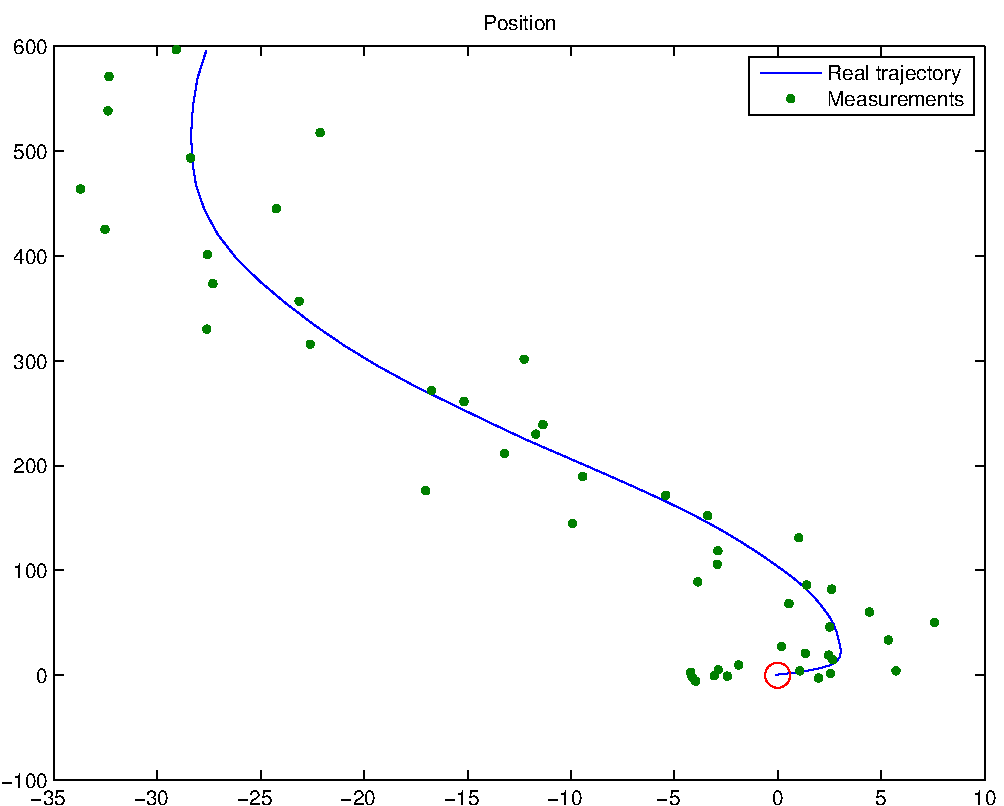
\includegraphics[width=11cm]{pics/demo1_f1}
\caption{The real position of the moving object and the simulated
  measurements of it using the CWPA model. The circle marks the
  starting point of the object.}
\label{fig:example1_1}
\end{center}
\end{figure}

The filtering is done with the following code fragment:
%
\begin{verbatim}
MM = zeros(size(m,1), size(Y,2));
PP = zeros(size(m,1), size(m,1), size(Y,2));

for i = 1:size(Y,2)
   [m,P] = kf_predict(m,P,A,Q);
   [m,P] = kf_update(m,P,Y(:,i),H,R);
   MM(:,i) = m;
   PP(:,:,i) = P;
end
\end{verbatim}
%
In the first 2 lines the space for state mean and covariance estimates is
reserved, and the rest of the code contains the actual filtering loop, where
we make the predict and update steps of the Kalman filter. The variables
\texttt{m} and \texttt{P} are assumed to contain the initial guesses for the
state mean and covariance before reaching the for-statement. Variable
\texttt{Y} is assumed to contain the measurements made from the system
(See the full source code of the example (\texttt{kf\_cwpa\_demo.m}) provided with the toolbox
to see how we generated the measurements by simulating the dynamic system). In
the end of each iteration the acquired estimates are stored to matrices
\texttt{MM} and \texttt{PP}, for which we reserved space earlier. The estimates
for object's position and velocity with Kalman filter and are plotted in figure
\ref{fig:example1_2}.\\

\begin{figure}
\begin{center}
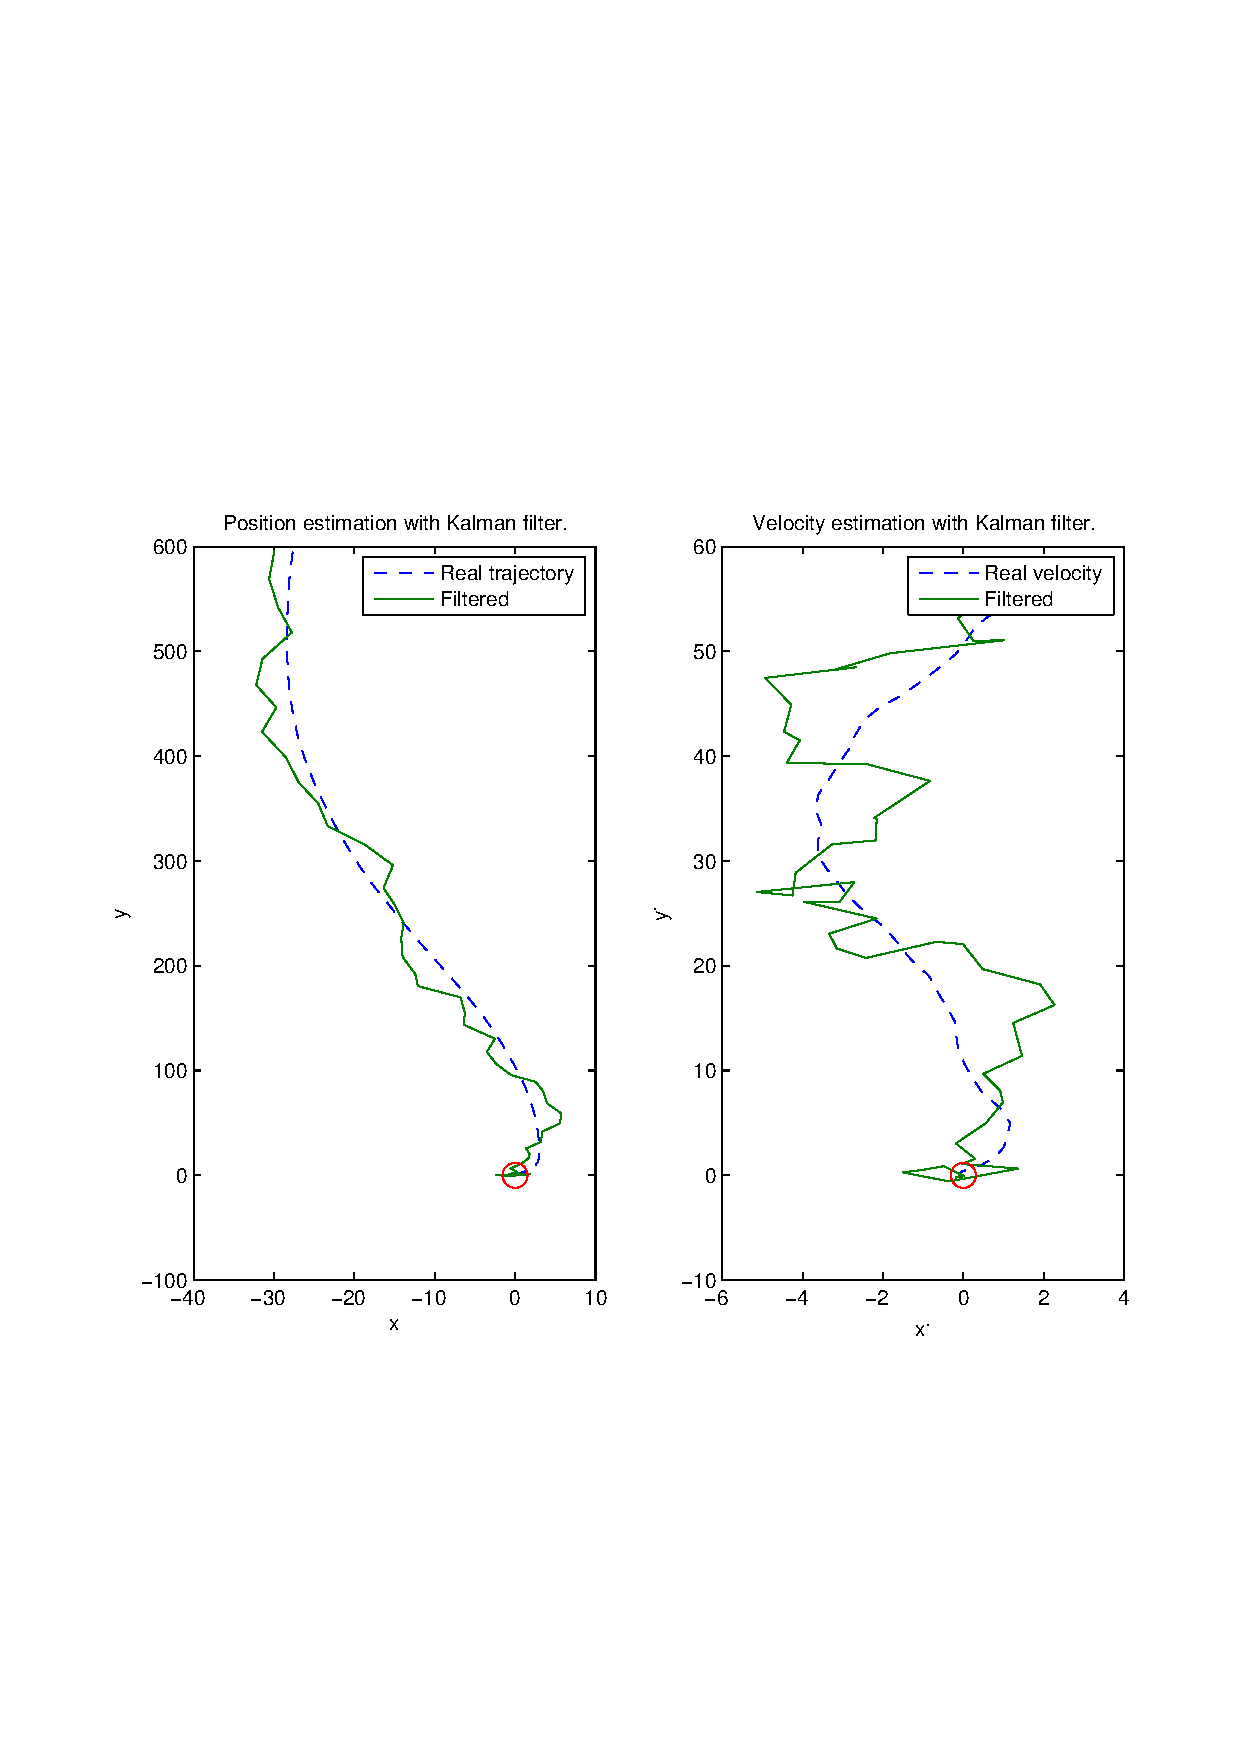
\includegraphics[width=11cm]{pics/demo1_f2}
\caption{Estimates for position and velocity of the moving object
  using the Kalman filter and CWPA model.}
\label{fig:example1_2}
\end{center}
\end{figure}

The smoothed estimates for the state mean and covariance can be calculated with the
following code line:
%
\begin{verbatim}
[SM,SP] = rts_smooth(MM,PP,A,Q);
\end{verbatim}
%
The calculated smoothed estimates for object's position and velocity for the
earlier demonstration are plotted in figure \ref{fig:example1_3}. As expected
the smoother produces more accurate estimates than the filter as it uses all
measurements for the estimation each time step. Note that the difference between
the smoothed and filtered estimated would be smaller, if the measurements were
more accurate, as now the filter performs rather badly due to the great
uncertaintity in the measurements. The smoothing results of a
forward-backward smoother are not plotted here, as the result are
exaclty the same as with the RTS smoother. 

As one would expect the estimates for object's velocity are clearly less
accurate than the estimates for the object's position as the positions are
observed directly and the velocities only indirectly. If the
velocities were also observed not only the velocity estimates would get
more accurate, but also the position ones as well. 

\begin{figure}
\begin{center}
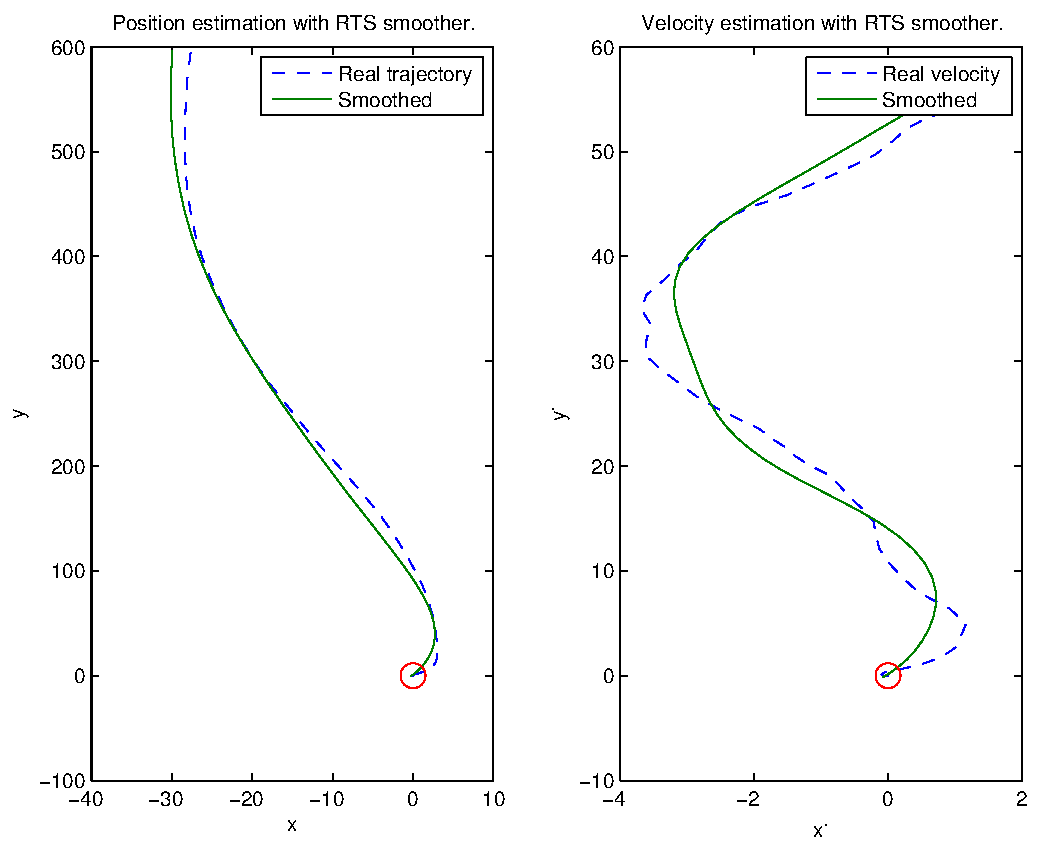
\includegraphics[width=11cm]{pics/demo1_f3}
\caption{Estimate for position and velocity of the moving object using the RTS smoother and CWPA model.}
\label{fig:example1_3}
\end{center}
\end{figure}

%%%%%%%%%%%%%%%%%%%%%%%%%%%%%%%%%%%%%%%%%%%%%%%%%%%%%%%%%%%%%%%%%%%%%%%%%%%%%%
%
\subsection{Nonlinear state space estimation}
%
%%%%%%%%%%%%%%%%%%%%%%%%%%%%%%%%%%%%%%%%%%%%%%%%%%%%%%%%%%%%%%%%%%%%%%%%%%%%%%

In many cases interesting dynamic systems are not by nature linear, so the
traditional Kalman filter cannot be applied in estimating the state of such a
system. In these kind of systems, both the dynamics and the measurement processes
can be nonlinear, or only one them. In this section, we describe two extensions
to the traditional Kalman filter, which can be applied for estimating nonlinear
dynamical systems by forming Gaussian approximations to the joint distribution of
the state $\vec{x}$ and measurement $\vec{y}$. First we present the Extended Kalman
filter (EKF), which is based on Taylor series approximation of the joint
distribution, and then the Unscented Kalman filter (UKF), which is
respectively based on the unscented transformation of the joint distribution.      


%%%%%%%%%%%%%%%%%%%%%%%%%%%%%%%%%%%%%%%%%%%%%%%%%%%%%%%%%%%%%%%%%%%%%%%%%%%%%%
%

\subsubsection{Taylor Series Based Approximations}

Next we present linear and quadratic approximations for the
distribution of variable $\vec{y}$, which is generated with a non-linear transformation
of a Gaussian random variable $\vec{x}$ as follows:
%
\begin{equation}
\begin{split}
  \vec{x} &\sim \N(\vec{m},\mat{P}) \\
  \vec{y} &= \vec{g}(\vec{x}).
\end{split}
\label{eq:trans_g}
\end{equation}
%
where $\vec{x} \in \spc{R}^n$, $\vec{y} \in \spc{R}^m$, and $\vec{g} :
\spc{R}^n \mapsto \spc{R}^m$ is a general non-linear function. Solving
the distribution of $\vec{y}$ formally is in general not possible,
because it is non-Gaussian for all by linear $\vec{g}$, so in practice
it must be approximated somehow. The joint distribution of $\vec{x}$
and $\vec{y}$ can be formed with, for example, linear and quadratic
approximations, which we present next. See, for example, (Bar-Shalom
et al., 2001) for the derivation of these approximations.

\subsubsection*{Linear Approximation}

The linear approximation based Gaussian approximation of the joint
distribution of variables $\vec{x}$ and $\vec{y}$ defined by equations (\ref{eq:trans_g})
is given as
  %
  \begin{equation}
     \begin{pmatrix}
       \vec{x} \\ \vec{y}
     \end{pmatrix} \sim
     \N\left(
     \begin{pmatrix}
       \vec{m} \\ \vecmu_L
     \end{pmatrix},
     \begin{pmatrix}
       \vec{P}   & \vec{C}_L \\
       \vec{C}_L^T & \mat{S}_L
     \end{pmatrix} \right),
  \end{equation}
  %
  where
  %
  \begin{equation}
  \begin{split}
  \vecmu_L &= \vec{g}(\vec{m}) \\
    \mat{S}_L &= \mat{G}_{\vec{x}}(\vec{m}) \, \mat{P} \,
    \mat{G}^T_{\vec{x}}(\vec{m}) \\
    \mat{C}_L &= \mat{P} \, \mat{G}^T_{\vec{x}}(\vec{m}),
  \end{split}
  \end{equation}
  %
  and $\mat{G}_{\vec{x}}(\vec{m})$ is the Jacobian matrix of $\vec{g}$
  with elements
  %
  \begin{equation}
    \left[ \mat{G}_{\vec{x}}(\vec{m}) \right]_{j,j'} =
    \frac{\partial g_j(\vec{x})}{\partial x_{j'}}
    \Bigg|_{\vec{x} = \vec{m}}.
  \label{eq:G1}
  \end{equation}

\subsubsection*{Quadratic Approximation}

The quadratic approximations retain also the second order terms of the
Taylor series expansion of the non-linear function:
  %
  \begin{equation}
     \begin{pmatrix}
       \vec{x} \\ \vec{y}
     \end{pmatrix} \sim
     \N\left(
     \begin{pmatrix}
       \vec{m} \\ \vecmu_Q
     \end{pmatrix},
     \begin{pmatrix}
       \vec{P}   & \vec{C}_Q \\
       \vec{C}_Q^T & \mat{S}_Q
     \end{pmatrix} \right),
  \end{equation}
  %
  where the parameters are
  %
  \begin{equation}
  \begin{split}
  \vecmu_Q &= \vec{g}(\vec{m}) 
  + \frac{1}{2} \sum_i \vec{e}_i \, \tr\left\{
     \mat{G}_{\vec{x}\vec{x}}^{(i)}(\vec{m}) \,
    \mat{P} \right\} \\
    \mat{S}_Q &= \mat{G}_{\vec{x}}(\vec{m}) \, \mat{P} \, \mat{G}^T_{\vec{x}}(\vec{m})
  + \frac{1}{2} \sum_{i,i'} \vec{e}_i \, \vec{e}^T_{i'} \,
    \tr\left\{ \mat{G}_{\vec{x}\vec{x}}^{(i)}(\vec{m}) \, \mat{P} \,
     \mat{G}_{\vec{x}\vec{x}}^{(i')}(\vec{m}) \, \mat{P} \right\} \\
    \mat{C}_Q &= \mat{P} \, \mat{G}^T_{\vec{x}}(\vec{m}),
  \end{split}
  \end{equation}
%
  $\mat{G}_{\vec{x}}(\vec{m})$ is the Jacobian matrix \eqref{eq:G1}
  and $\mat{G}_{\vec{x}\vec{x}}^{(i)}(\vec{m})$ is the Hessian matrix
  of $g_i(\cdot)$ evaluated at $\vec{m}$:
%
\begin{equation}
   \left[ \mat{G}_{\vec{x}\vec{x}}^{(i)}(\vec{m}) \right]_{j,j'}
   = \frac{\partial^2 g_i(\vec{x})}{\partial x_j \, \partial x_{j'}},
  \Bigg|_{\vec{x} = \vec{m}}.
\end{equation}
%
$\vec{e}_i = (0~\cdots~0~1~0~\cdots~0)^T$ is the unit
vector in direction of the coordinate axis $i$.



\subsubsection{Extended Kalman filter}
%
%%%%%%%%%%%%%%%%%%%%%%%%%%%%%%%%%%%%%%%%%%%%%%%%%%%%%%%%%%%%%%%%%%%%%%%%%%%%%%

The extended Kalman filter (see, for instance, Jazwinski, 1970; Maybeck, 1982a;
Bar-Shalom et al., 2001; Grewal and Andrews, 2001; S�rkk�, 2006) extends the scope
of Kalman filter to nonlinear optimal filtering problems by forming a Gaussian
approximation to the joint distribution of state $\vec{x}$ and measurements
$\vec{y}$ using a Taylor series based transformation. First and second order
extended Kalman filters are presented, which are based on linear and quadratic
approximations to the transformation. Higher order filters are also possible,
but not presented here.


The filtering model used in the EKF is
%
\begin{equation}
\begin{split}
\vec{x}_{k} &= \vec{f}(\vec{x}_{k-1},k-1) + \vec{q}_{k-1} \\
\vec{y}_{k} &= \vec{h}(\vec{x}_{k},k) + \vec{r}_{k},
\end{split} \label {eq:nonlinear_prob}
\end{equation}
%
where $\vec{x}_k \in \spc{R}^n$ is the state, $\vec{y}_k \in \spc{R}^m$
is the measurement,  $\vec{q}_{k-1} \sim \N(\vec{0},\mat{Q}_{k-1})$ is
the process noise, $\vec{r}_{k} \sim \N(\vec{0},\mat{R}_{k})$ is the
measurement noise, $\vec{f}$ is the (possibly nonlinear) dynamic model
function and $\vec{h}$ is the (again possibly nonlinear) measurement model
function. The first and second order extended Kalman filters approximate the
distribution of state $\vec{x}_k$ given the observations $\vec{y}_{1:k}$
with a Gaussian:
%
\begin{equation}
  p(\vec{x}_{k}\,|\,\vec{y}_{1:k}) \approx
    \N(\vec{x}_{k}\,|\,\vec{m}_{k},\mat{P}_{k}).
\end{equation}
%

\subsubsection*{First Order Extended Kalman Filter}

Like Kalman filter, also the extended Kalman filter is separated to two steps.
The steps for the first order EKF are as follows:
  %
  \begin{itemize}
  \item {\em Prediction:}
  %
  \begin{equation}
  \begin{split}
    \vec{m}^-_{k} &= \vec{f}(\vec{m}_{k-1},k-1) \\
    \mat{P}^-_{k} &= \mat{F}_{\vec{x}}(\vec{m}_{k-1},k-1) \, \mat{P}_{k-1} \,
     \mat{F}_{\vec{x}}^T (\vec{m}_{k-1},k-1) + \mat{Q}_{k-1}.
  \end{split}
  \label{eq:dekf_predict1}
  \end{equation}
  
  \item {\em Update:}
  %
  \begin{equation}
  \begin{split}
    \vec{v}_{k} &= \vec{y}_k - \mat{h} (\vec{m}^-_{k},k) \\
    \vec{S}_{k} &= \mat{H}_{\vec{x}}(\vec{m}^-_{k},k) \, \mat{P}^-_{k} \,
    \mat{H}^T_{\vec{x}}(\vec{m}^-_{k},k) + \vec{R}_{k} \\
    \vec{K}_{k} &= \mat{P}^-_{k} \, \mat{H}^T_{\vec{x}}(\vec{m}^-_{k},k) \,
    \vec{S}^{-1}_{k} \\
    \vec{m}_{k} &= \vec{m}^-_{k} + \vec{K}_{k} \, \vec{v}_k \\
    \mat{P}_{k} &= \mat{P}^-_{k} - \vec{K}_{k} \, \vec{S}_{k} \, \vec{K}^T_{k},
  \end{split}
  \label{eq:dekf_update1}
  \end{equation}
  \end{itemize}
  %
  where the matrices $\mat{F}_{\vec{x}}(\vec{m},k-1)$ and
  $\mat{H}_{\vec{x}}(\vec{m},k)$ are the Jacobians of
  $\vec{f}$ and $\vec{h}$, with elements
  %
  \begin{align}
    \left[ \mat{F}_{\vec{x}}(\vec{m},k-1) \right]_{j,j'} =
    \frac{\partial f_j(\vec{x},k-1)}{\partial x_{j'}}
    \Bigg|_{\vec{x} = \vec{m}}
  \label{eq:F1} \\
    \left[ \mat{H}_{\vec{x}}(\vec{m},k) \right]_{j,j'} =
    \frac{\partial h_j(\vec{x},k)}{\partial x_{j'}}
    \Bigg|_{\vec{x} = \vec{m}}.
  \label{eq:H1}
  \end{align}
%
Note that the difference between first order EKF and KF is that the
matrices $\mat{A}_k$ and $\mat{H}_k$ in KF are replaced with Jacobian
matrices $\mat{F}_{\vec{x}}(\vec{m}_{k-1},k-1)$ and
$\mat{H}_{\vec{x}}(\vec{m}_k^-,k)$ in EKF. Predicted mean
$\vec{m}_k^-$ and residual of prediction $\vec{v}_k$ are also calculated differently in the EKF.  

\subsubsection*{Second Order Extended Kalman Filter}

The corresponding steps for the second order EKF are as follows:
  %
  \begin{itemize}
  \item {\em Prediction:}
  %
  \begin{equation}
  \begin{split}
    \vec{m}^-_{k} &= \vec{f}(\vec{m}_{k-1},k-1) 
    + \frac{1}{2} \sum_i \vec{e}_i \,
      \tr\left\{ \mat{F}_{\vec{x}\vec{x}}^{(i)}(\vec{m}_{k-1},k-1) \,
      \mat{P}_{k-1} \right\} \\
    \mat{P}^-_{k} &= \mat{F}_{\vec{x}}(\vec{m}_{k-1},k-1) \, \mat{P}_{k-1} \,
     \mat{F}^T_{\vec{x}}(\vec{m}_{k-1},k-1) \\
   &+ \frac{1}{2} \sum_{i,i'} \vec{e}_i \, \vec{e}^T_{i'}
      \tr\left\{ \mat{F}_{\vec{x}\vec{x}}^{(i)}(\vec{m}_{k-1},k-1) \mat{P}_{k-1} 
       \mat{F}_{\vec{x}\vec{x}}^{(i')}(\vec{m}_{k-1},k-1) \mat{P}_{k-1} \right\} \\
    &+ \mat{Q}_{k-1}.
  \end{split}
  \label{eq:dekf_predict2}
  \end{equation}

  \item {\em Update:}
  %
  \begin{equation}
  \begin{split}
    \vec{v}_{k} &= \vec{y}_k - \mat{h} (\vec{m}^-_{k},k) 
    - \frac{1}{2} \sum_i \vec{e}_i \,
      \tr\left\{ \mat{H}_{\vec{x}\vec{x}}^{(i)}(\vec{m}^-_{k},k) \,
      \mat{P}^-_{k} \right\} \\
    \vec{S}_{k} &= \mat{H}_{\vec{x}}(\vec{m}^-_{k},k) \, \mat{P}^-_{k} \,
    \mat{H}^T_{\vec{x}}(\vec{m}^-_{k},k) \\
    &\quad + \frac{1}{2} \sum_{i,i'} \vec{e}_i \, \vec{e}^T_{i'} \,
      \tr\left\{ \mat{H}_{\vec{x}\vec{x}}^{(i)}(\vec{m}^-_{k},k) \, \mat{P}^-_{k} \,
       \mat{H}_{\vec{x}\vec{x}}^{(i')}(\vec{m}^-_{k},k) \, \mat{P}^-_{k} \right\} 
    + \vec{R}_{k} \\
    \vec{K}_{k} &= \mat{P}^-_{k} \,
    \mat{H}^T_{\vec{x}}(\vec{m}^-_{k},k) \, \vec{S}^{-1}_{k} \\
    \vec{m}_{k} &= \vec{m}^-_{k} + \vec{K}_{k} \, \vec{v}_k \\
    \mat{P}_{k} &= \mat{P}^-_{k} - \vec{K}_{k} \, \vec{S}_{k} \, \vec{K}^T_{k},
  \end{split}
  \label{eq:dekf_update2}
  \end{equation}
  \end{itemize}
  %
  where matrices $\mat{F}_{\vec{x}}(\vec{m},k-1)$ and
  $\mat{H}_{\vec{x}}(\vec{m},k)$ are Jacobians as in the first order EKF, given by
  Equations \eqref{eq:F1} and \eqref{eq:H1}. The matrices
  $\mat{F}^{(i)}_{\vec{x}\vec{x}}(\vec{m},k-1)$ and
  $\mat{H}^{(i)}_{\vec{x}\vec{x}}(\vec{m},k)$ are the Hessian matrices
  of $f_i$ and $h_i$:
  \begin{align}
   \left[ \mat{F}_{\vec{x}\vec{x}}^{(i)}(\vec{m},k-1) \right]_{j,j'}
   = \frac{\partial^2 f_i(\vec{x},k-1)}{\partial x_j \, \partial x_{j'}}
  \Bigg|_{\vec{x} = \vec{m}}
  \label{eq:F2} \\
   \left[ \mat{H}_{\vec{x}\vec{x}}^{(i)}(\vec{m},k) \right]_{j,j'}
   = \frac{\partial^2 h_i(\vec{x},k)}{\partial x_j \, \partial x_{j'}}
  \Bigg|_{\vec{x} = \vec{m}},
  \label{eq:H2}
  \end{align}
%
$\vec{e}_i = (0~\cdots~0~1~0~\cdots~0)^T$ is a unit vector in direction of the
coordinate axis $i$, that is, it has a $1$ at position $i$ and $0$ at other positions.

The prediction and update steps of the second order EKF can be computed
in this toolbox with functions \texttt{ekf\_predict2} and
\texttt{ekf\_update2}, respectively. By taking the second order terms
into account, however, doesn't quarantee, that the results get any
better. Depending on problem they might even get worse, as we shall
see in the later examples.
\subsubsection*{The Limitations of EKF}

As discussed in, for example, (Julier and Uhlmann, 2004) the EKF has a
few serious drawbacks, which should be kept in mind when it's used:
%
\begin{enumerate}
\item As we shall see in some of the later demonstrations, the linear
  and quadratic transformations produces realiable results only
  when the error propagation can be well approximated by a linear or a
  quadratic function. If this condition is not met, the performance of the 
  filter can be extremely poor. At worst, its estimates can diverge altogether.
\item The Jacobian matrices (and Hessian matrices with second order
  filters) need to exist so that the transformation can be
  applied. However, there are cases, where this isn't true. For
  example, the system might be jump-linear, in which the parameters can
  change abruptly (Julier and Uhlmann, 2004). 
\item In many cases the calculation of Jacobian and Hessian matrices can be a very
  difficult process, and its also prone to human errors (both
  derivation and programming). These errors are usually very hard to
  debug, as its hard to see which parts of the system produces the
  errors by looking at the estimates, especially as
  usually we don't know which kind of performance we should
  expect. For example, in the last demonstration (Reentry Vehicle
  Tracking) the first order derivatives were quite troublesome to
  calcute, even though the equations themselves were relatively
  simple. The second order derivatives would have even taken many more
  times of work.  
\end{enumerate}
%
\label{page:ekf_problems}


  

%%%%%%%%%%%%%%%%%%%%%%%%%%%%%%%%%%%%%%%%%%%%%%%%%%%%%%%%%%%%%%%%%%%%%%%%%%%%%%
%
\subsubsection{Extended Kalman smoother}
%
%%%%%%%%%%%%%%%%%%%%%%%%%%%%%%%%%%%%%%%%%%%%%%%%%%%%%%%%%%%%%%%%%%%%%%%%%%%%%%

The difference between the first order extended Kalman smoother (Cox, 1964;
Sage and Melsa, 1971) and the traditional Kalman smoother is the same as the
difference between first order EKF and KF, that is, matrix $\mat{A}_k$ in
Kalman smoother is replaced with Jacobian
$\mat{F}_{\vec{x}}(\vec{m}_{k-1},k-1)$, and $\vec{m}_{k+1}^-$ is
calculated using the model function $\vec{f}$. 
Thus, the equations for the extended Kalman smoother can be written as
%
\begin{equation}
\begin{split}
    \vec{m}^-_{k+1} &= \vec{f}(\vec{m}_{k},k) \\
    \mat{P}^-_{k+1} &= \mat{F}_{\vec{x}}(\vec{m}_{k},k) \, \mat{P}_{k} \,
     \mat{F}_{\vec{x}}^T(\vec{m}_{k},k) + \mat{Q}_{k} \\
    \vec{C}_{k} &= \mat{P}_k \, \mat{F}_{\vec{x}}^T(\vec{m}_{k},k) \,
      [\mat{P}^-_{k+1}]^{-1} \\
    \vec{m}^s_k &= \vec{m}_k
    + \mat{C}_k \, [\vec{m}^s_{k+1} - \vec{m}^-_{k+1}] \\
    \mat{P}^s_k &= \mat{P}_k
    + \mat{C}_k \, [\mat{P}^s_{k+1} - \mat{P}^-_{k+1}] \, \mat{C}^T_k.
    \label{eq:derts}
\end{split}
\end{equation}
%
First order smoothing solutiong with a RTS type smoother can be computed with function
\texttt{erts\_smooth1}, and with forward-backward type smoother the
computation can be done with function \texttt{efbf\_smooth1}.

Higher order smoothers are also possible, but not described here, as they are not
currently implemented in this toolbox.

%%%%%%%%%%%%%%%%%%%%%%%%%%%%%%%%%%%%%%%%%%%%%%%%%%%%%%%%%%%%%%%%%%%%%%%%%%%%%%
%
\subsubsection{Demonstration: Tracking a random sine signal}
%
%%%%%%%%%%%%%%%%%%%%%%%%%%%%%%%%%%%%%%%%%%%%%%%%%%%%%%%%%%%%%%%%%%%%%%%%%%%%%%
Next we consider a simple, yet practical, example of a nonlinear dynamic
system, in which we estimate a random sine signal using the extended
Kalman filter. By random we mean that the angular velocity and the amplitude
of the signal can vary through time. In this example the nonlinearity in the
system is expressed through the measurement model, but it would also be possible
to express it with the dynamic model and let the measurement model be linear.

The state vector in this case can be expressed as
%
\begin{equation}
%
\vec{x}_k = 
\begin{pmatrix}
\theta_k & \omega_k & a_k
\end{pmatrix}^T,
%
\end{equation}
%
where $\theta_k$ is the parameter for the sine function on time step $k$,
$\omega_k$ is the angular velocity on time step $k$ and $a_k$ is the amplitude
on time step $k$. The evolution of parameter $\theta$ is modelled with a
discretized Wiener velocity model, where the velocity is now the angular velocity:
%
\begin{equation}
%
\frac{d \theta}{d t} = \omega.
%
\end{equation}
%
The values of $\omega$ and $a$ are perturbed with one dimensional white noise
processes $w_a(t)$ and $w_w(t)$, so the signal
isn't totally deterministic:
%
\begin{eqnarray}
%
\frac{da}{dt} &=& w_a(t) \\
\frac{dw}{dt} &=& w_w(t).
%
\end{eqnarray}
%
Thus, the continous-time dynamic equation can be
written as
%
\begin{equation}
%
\frac{d \vec{x}(t)}{dt} = \begin{pmatrix}
0 & 1 & 0\\
0 & 0 & 0\\
0 & 0 & 0
\end{pmatrix}\vec{x}(t)
+
\begin{pmatrix}
0 & 0 \\
1 & 0 \\
0 & 1
\end{pmatrix}\vec{w}(t), \label{eq:sine_cont_model}
%
\end{equation}
%
where the white noise process $\vec{w}(t)$ has power spectral density
%
\begin{equation}
%
\mat{Q}_c =  \begin{pmatrix}
q_1 & 0 \\
0 & q_2 
\end{pmatrix}.
%
\end{equation}
%
Variables $q_1$ and $q_2$ describe the strengths of random perturbations of the angular
velocity and the amplitude, respectively, which are in this demonstration
are set to $q_1 = 0.2$ and $q_2 = 0.1$. By using the equation (\ref{eq:ode_ak})
the discretized form of the dynamic equation can written as
%
\begin{equation}
%
\vec{x}_k = \begin{pmatrix}
1 & \dt & 0\\
0 & 1 & 0\\
0 & 0 & 1
\end{pmatrix}\vec{x}_{k-1}
+
\vec{q}_{k-1},
%
\end{equation}
%
where $\dt$ is the step size (with value $\dt = 0.01$ in this case),
and using the equation (\ref{eq:ode_qk}) the
covariance matrix $\mat{Q}_{k-1}$ of the discrete Gaussian white noise process
$\vec{q}_{k-1} \sim N(\vec{0},\mat{Q}_{k-1})$ can be easily computed
to give 
%
\begin{equation}
%
\mat{Q}_{k-1} = \begin{pmatrix}
\frac{1}{3}\dt^3q_1 & \frac{1}{2}\dt^2q_1 & 0\\
\frac{1}{2}\dt^2q_1 & \dt q_1             & 0\\
0                   & 0                   & \dt q_2
\end{pmatrix}.
\end{equation}
%

As stated above, the non-linearity in this case is expressed by the measurement
model, that is, we propagate the current state through a non-linear measurement function
$\vec{h}(\vec{x}_{k},k)$ to get an actual measurement. Naturally the function in this
case is the actual sine function
%
\begin{equation}
%
\vec{h}(\vec{x}_{k},k) = a_k\sin(\theta_k). \label{eq:ekf_demo1_h}
%
\end{equation}
%
With this the measurement model can be written as
%
\begin{equation}
%
y_k = \vec{h}(\vec{x}_k,k) + r_k = a_k\sin(\theta_k) + r_k,
%
\end{equation}
%
where $r_k$ is white, univariate Gaussian noise with zero mean and variance
$\sigma_r = 1$.
 
The derivatives of the measurement function with respect to state variables are
%
\begin{equation}
\begin{split}
%
\frac{\partial \vec{h}(\vec{x}_{k},k)}{\partial \theta_k} &= a_k\cos(\theta_k)\\
\frac{\partial \vec{h}(\vec{x}_{k},k)}{\partial \omega_k} &= 0\\
\frac{\partial \vec{h}(\vec{x}_{k},k)}{\partial a_k} &= \sin(\theta_k),
%
\end{split}
\end{equation}
%
so the Jacobian matrix (actually in this case, a vector, as the measurements are only
one dimensional) needed by the EKF can be written as
%
\begin{equation}
%
\mat{H}_{\vec{x}}(\vec{m},k) = \begin{pmatrix}
a_k\cos(\theta_k) & 0 & \sin(\theta_k) \label{eq:ekf_demo1_jacobian}
\end{pmatrix}.
%
\end{equation}
%

We also filter the signal with second order EKF, so we need to
evaluate the Hessian matrix of the measurement model function.
In this case the second order derivatives of $\vec{h}$ with respect to
all state variables can written as

\begin{equation}
\begin{split}
%
\frac{\partial^2 \vec{h}(\vec{x}_{k},k)}{\partial \theta_k \partial \theta_k} &= -a_k\sin(\theta_k)\\
\frac{\partial^2 \vec{h}(\vec{x}_{k},k)}{\partial \theta_k \partial \omega_k} &= 0\\
\frac{\partial^2 \vec{h}(\vec{x}_{k},k)}{\partial \theta_k \partial a_k} &= \cos(\theta_k)\\
\frac{\partial^2 \vec{h}(\vec{x}_{k},k)}{\partial \omega_k \partial \omega_k} &= 0\\
\frac{\partial^2 \vec{h}(\vec{x}_{k},k)}{\partial \omega_k \partial a_k} &= 0\\
\frac{\partial^2 \vec{h}(\vec{x}_{k},k)}{\partial a_k \partial a_k} &= 0.
%
\end{split}
\end{equation}
With these the Hessian matrix can expressed as
%
\begin{equation}
%
\mat{H}_{\vec{xx}}(\vec{m},k) = \begin{pmatrix}
-a_k\sin(\theta_k) & 0 & \cos(\theta_k) \\
0 & 0 & 0 \\
\cos(\theta_k) & 0 & 0  \label{eq:ekf_demo1_hessian}
\end{pmatrix}.
%
\end{equation}
%
Note that as the measurements are only one dimensional we need to
evaluate only one Hessian, and as the expressions are rather simple the computation
of this Hessian is trivial. In case of higher dimensions we would need to evaluate
the Hessian for each dimension separately, which could easily result in high
amount of dense algebra.


In this demonstration program the measurement function
(\ref{eq:ekf_demo1_h}) is computed with the following code:
%
\begin{verbatim}
function Y = ekf_demo1_h(x,param)
f = x(1,:);
a = x(3,:);
Y = a.*sin(f);
if size(x,1) == 7
    Y = Y + x(7,:);
end
\end{verbatim}
%
where the parameter \texttt{x} is a vector containing a single state
value, or a matrix containing multiple state values. It is also
necessary to include the parameter \texttt{param}, which contains the
other possible parameters for the functions (not present in this
case). The last three lines are included for the augmented version of unscented Kalman
filter (UKF), which is described later in this document.
The Jacobian matrix of the measurement function (eq.
(\ref{eq:ekf_demo1_jacobian})) is
computed with the following function:
%
\begin{verbatim}
function dY = ekf_demo1_dh_dx(x, param)
f = x(1,:);
w = x(2,:);
a = x(3,:);
dY = [(a.*cos(f))' zeros(size(f,2),1) (sin(f))'];
\end{verbatim}
%
The Hessian matrix of the measurement function (eq.
\ref{eq:ekf_demo1_hessian}) is computed with the following function:
%
\begin{verbatim}
function df = ekf_sine_d2h_dx2(x,param)
f = x(1);
a = x(3);

df = zeros(1,3,3);
df(1,:,:) = [-a*sin(f) 0 cos(f);
             0         0      0;
             cos(f)    0      0];
\end{verbatim}
% 
These functions are defined in files \texttt{efk\_sine\_h.m},
\texttt{ekf\_sine\_dh\_dx.m} and \texttt{ekf\_sine\_d2h\_dx2.m},
respectively. The handles of these functions are saved in the actual
demonstration script file (\texttt{ekf\_sine\_demo.m}) with the following code lines:
%
\begin{verbatim}
h_func = @ekf_sine_h;
dh_dx_func = @ekf_sine_dh_dx;
d2h_dx2_func = @ekf_sine_d2h_dx2;
\end{verbatim}
%

It is also important to check out that the implementation on calculating
the derivatives is done right, as it is, especially with more complex
models, easy to make errors in the equations. This can be done with function
\texttt{der\_check} (see page \pageref{page:der_check} for more details):
%
\begin{verbatim}
der_check(h_func, dh_dx_func, 1, [f w a]');
\end{verbatim}
%
The third parameter with value \texttt{1} signals that we want to test
the derivative of function's first (and in this case the only) dimension.
Above we have assumed, that the variable \texttt{f} contains the
parameter value for the sine function, \texttt{w} the angular velocity
of the signal and \texttt{a} the amplitude of the signal. 

After we have discretized the dynamic model and generated the real states and
measurements same as in the previous example (the actual code lines
are not stated here, see the full source code at end of this
document), we can use the EKF to get the filtered estimates for the
state means and covariances. The filtering (with first order EKF) is done almost the same as
in the previous example:
%
\begin{verbatim}
  MM = zeros(size(M,1),size(Y,2));
  PP = zeros(size(M,1),size(M,1),size(Y,2));

  for k=1:size(Y,2)
     [M,P] = ekf_predict1(M,P,A,Q);
     [M,P] = ekf_update1(M,P,Y(:,k),dh_dx_func,R*eye(1),h_func);
     MM(:,k)   = M;
     PP(:,:,k) = P;
  end
\end{verbatim}
%
As the model dynamics are in this case linear the prediction step
functions exactly the same as in the case of traditional Kalman
filter. In update step we pass the handles to
the measurement model function and it's derivative function and the
variance of measurement noise (parameters 6, 4 and 5,
respectively), in addition to other parameters. These functions also
have additional parameters, which might be needed in some cases. For example,
the dynamic and measurement model functions might have parameters,
which are needed when those functions are called. See the full
function specifications in section 3 for more details about the parameters. 

With second order EKF the filtering loop remains almost the same with
the exception of update step:
%
\begin{verbatim}
  MM2 = zeros(size(M,1),size(Y,2));
  PP2 = zeros(size(M,1),size(M,1),size(Y,2));

  for k=1:size(Y,2)
     [M,P] = ekf_predict1(M,P,A,Q);
     [M,P] = ekf_update2(M,P,Y(:,k),dh_dx_func,...
                         d2h_dx2_func,R*eye(1),h_func);
     MM(:,k)   = M;
     PP(:,:,k) = P;
  end
\end{verbatim}
%


The smoothing of state estimates using the extended RTS smoother is done
sameways as in the previous example:
%
\begin{verbatim}  
[SM1,SP1] = erts_smooth1(MM,PP,A,Q);
\end{verbatim}
%
With the extended forward-backward smoother the smoothing is done with
the following function call:
%
\begin{verbatim}
[SM2,SP2] = efbf_smooth1(MM,PP,Y,A,Q,[],[],[],...
                         dh_dx_func,R*eye(1),h_func);
\end{verbatim}
%
Here we have assigned empty vectors for parameters 6,7 and 8 (inverse
prediction, its derivative w.r.t. to noise and its parameters, respectively),
because they are not needed in this case.

To visualize the filtered and smoothed signal estimates we must evaluate
the measurement model function with every state estimate to project the
estimates to the measurement space. This can be done with the built-in
Matlab function \texttt{feval}:
%
\begin{verbatim}
Y_m = feval(h_func, MM);
\end{verbatim}
%
The filtered and smoothed estimates of the signals using the first
order EKF, ERTS and EFBF are plotted in
figures \ref{fig:example2_1}, \ref{fig:example2_2} and
\ref{fig:example2_3}, respectively. The estimates produced by second order EKF are
not plotted as they do not differ much from first order ones.
As can be seen from the figures both smoothers give clearly better
estimates than the filter. Especially in the beginning of the signal
it takes a while for the filter to catch on to right track. 


\label{page:sine_rmse}

The difference between the smoothers doesn't become clear just by
looking these figures. In some cases the forward-backward smoother
gives a little better estimates, but it tends to be more sensitive
about numerical accuracy and the process and measurement noises. 
To make a comparison between the performances of different methods we
have listed the average of root mean square errors (RMSE) on 100 Monte Carlo
simulations with different methods in table \ref{table:sine_errors}.
In addition to RMSE of each state variable we also provide the
estimation error in measurement space, because we might be
more interested in estimating the actual value of signal than its components.
Usually, however, the primary goal of these methods is to estimate the
hidden state variables. The following methods were used:
%
\begin{itemize}
\item EKF1: First order extended Kalman filter.
\item ERTS1: First order extended Rauch-Tung-Striebel smoother.
\item EFBF1: First order extended Forward-Backward smoother.
\item EKF2: Second order extended Kalman filter.
\item ERTS2: First order extended Rauch-Tung-Striebel smoother applied
  to second order EKF estimates.
\item EFBF2: First order extended Forward-Backward smoother applied to
  second order EKF estimates.
\item UKF: unscented Kalman filter.
\item URTS: unscented Rauch-Tung-Striebel smoother.
\end{itemize}
%
From the errors we can see that with filters EKF2 gives clearly the lowest
errors with variables $\theta$ and $a$. Due to this also with
smoothers ERTS2 and EFBF2 give clearly lower errors than others. 
On the other hand EKF1 gives the lowest estimation error
with variable $\omega$. Furthermore, with filters EKF1 also gives lowest error in
measurement space. Each smoother, however, gives approximately the
same error in measurement space. It can also be seen, that the UKF
functions the worst in this case. This is due to linear and quadratic
approximations used in EKF working well with this model. However, with
more nonlinear models UKF is often superior over EKF, as we shall see
in later sections. 

In all, none of the used methods proved to be
clearly superior over the others with this model. It is clear,
however, that EKF should be preferred over UKF as it gives lower error
and is slightly less demanding in terms of computation power.
Whether first or second order EKF should be used is ultimately up to the goal of
application. If the actual signal value is of interest, which is usually
the case, then one should use first order EKF, but second order one
might better at predicting new signal values as the variables $\theta$
and $a$ are closer to real ones on average. 

\begin{figure}
\begin{center}
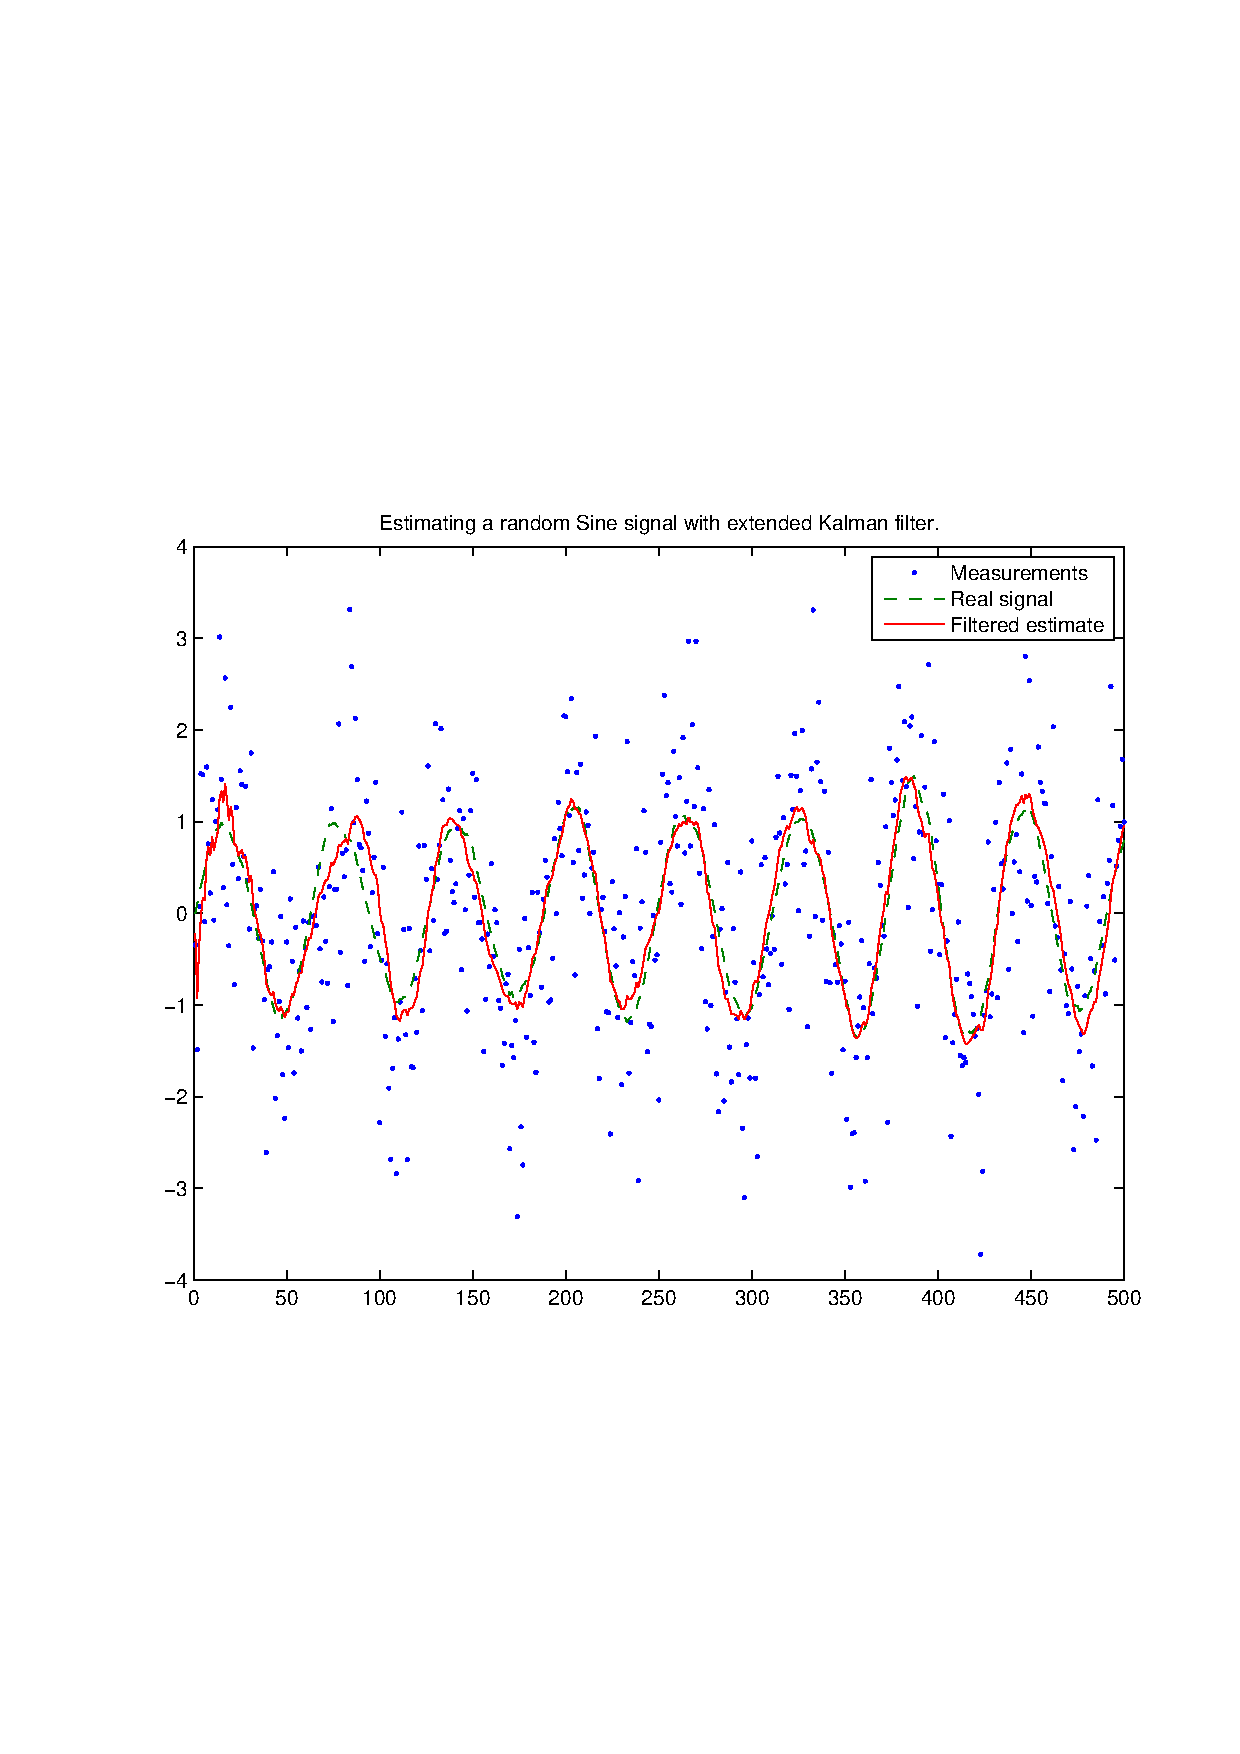
\includegraphics[width=11cm]{pics/demo2_f1}
\caption{Filtered estimate of the sine signal using the first order extended Kalman filter.}
\label{fig:example2_1}
\end{center}
\end{figure}

\begin{figure}
\begin{center}
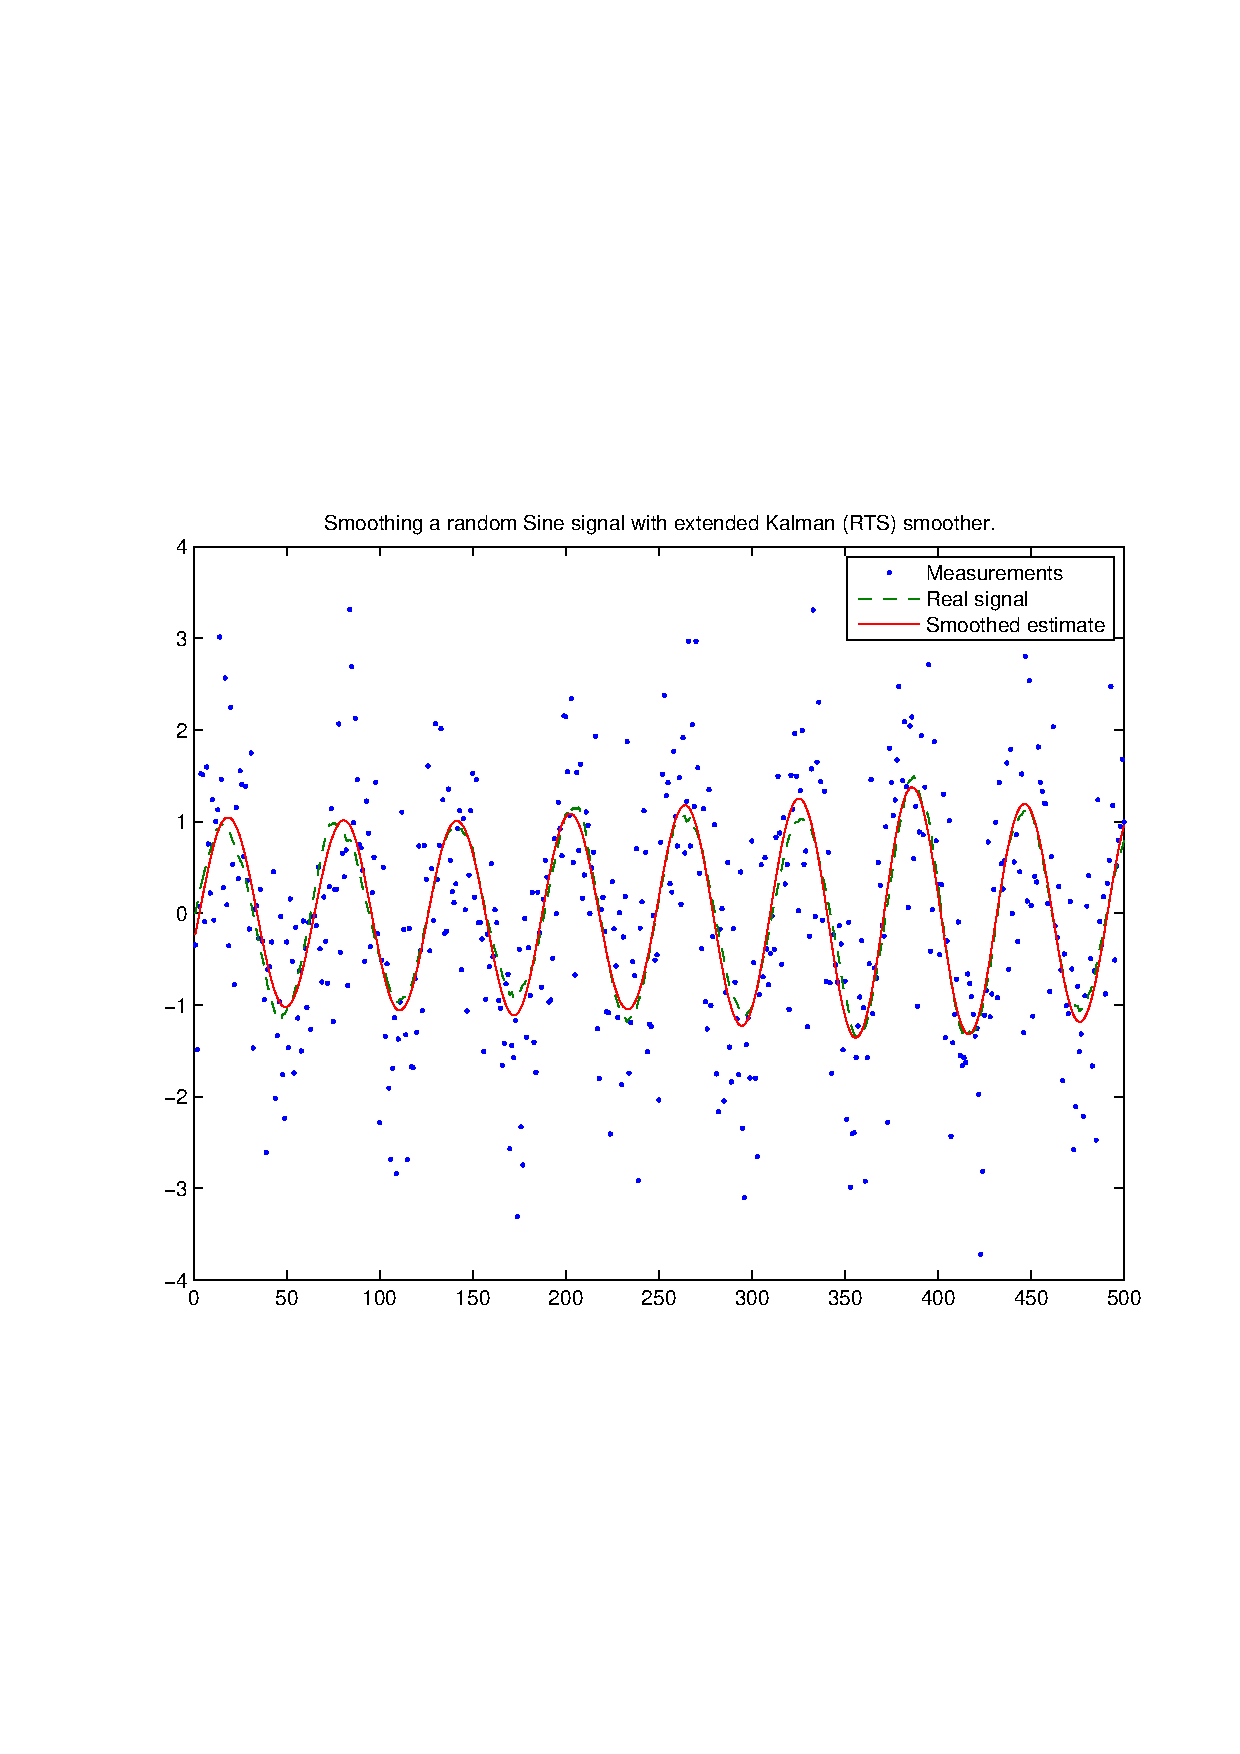
\includegraphics[width=11cm]{pics/demo2_f2}
\caption{Smoothed estimate of the sine signal using the extended Kalman (RTS) smoother.}
\label{fig:example2_2}
\end{center}
\end{figure}

\begin{figure}
\begin{center}
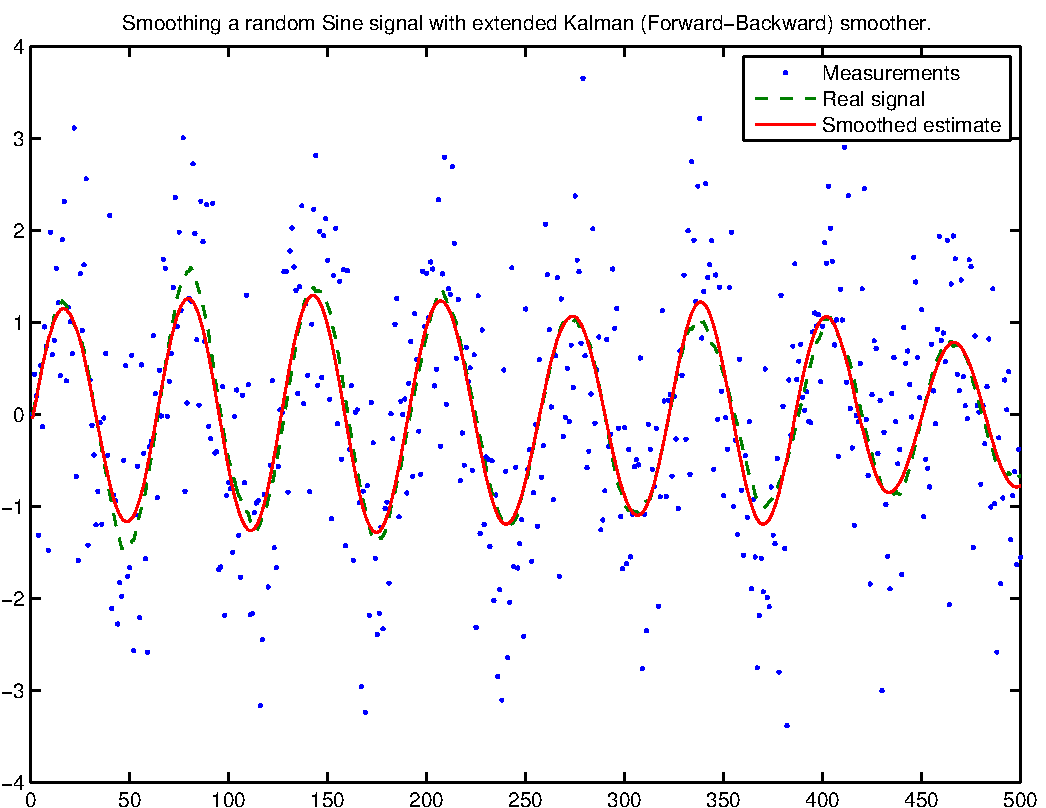
\includegraphics[width=11cm]{pics/demo2_f3}
\caption{Smoothed estimate of the sine signal using the extended Kalman (Forward-Backward) smoother.}
\label{fig:example2_3}
\end{center}
\end{figure}


\begin{table}
\begin{center}
\begin{tabular}{|l|l|l|l|l|l|}
\hline
{\it Method}&{\it RMSE[$\theta$]}&{\it RMSE[$\omega$]}&{\it
  RMSE[$a$]}& {\it RMSE[$y$]}\\
\hline
EKF1 & 0.64 & 0.53 & 0.40 & 0.24 \\
ERTS1& 0.52 & 0.31 & 0.33 & 0.15 \\
EFBF1& 0.53 & 0.31 & 0.34 & 0.15 \\
EKF2 & 0.34 & 0.54 & 0.31 & 0.29 \\
ERTS2& 0.24 & 0.30 & 0.18 & 0.15 \\
EFBF2& 0.24 & 0.30 & 0.18 & 0.15 \\
UKF  & 0.59 & 0.56 & 0.39 & 0.27 \\
URTS & 0.45 & 0.30 & 0.30 & 0.15 \\ 
\hline   
\end{tabular}
\caption{RMSEs of estimating the random sinusoid over 100 Monte Carlo simulations.}
\label{table:sine_errors}
\end{center}
\end{table} 



%%%%%%%%%%%%%%%%%%%%%%%%%%%%%%%%%%%%%%%%%%%%%%%%%%%%%%%%%%%%%%%%%%%%%%%%%%%%%%
%
\subsubsection{Unscented Transform}
%
%%%%%%%%%%%%%%%%%%%%%%%%%%%%%%%%%%%%%%%%%%%%%%%%%%%%%%%%%%%%%%%%%%%%%%%%%%%%%%

Like Taylor series based approximation presented above also the {\it unscented
  transform} (UT) (Julier and Uhlmann, 1995, 2004; Wan and van der
Merwe, 2001) can be used for forming a Gaussian approximation to the
joint distribution of random variables $\vec{x}$ and $\vec{y}$, which
are defined with equations (\ref{eq:trans_g}). In UT we
deterministically choose a fixed number of sigma points, which capture
the desired moments (atleast mean and covariance) of the original
distribution of $\vec{x}$ exactly. After that we propagate the sigma
points through the non-linear function $\vec{g}$ and estimate the
moments of the transformed variable from them. 

The advantage of UT over the Taylor series based
approximation is that UT is better at capturing the higher order
moments caused by the non-linear transform, as discussed in (Julier
and Uhlmann, 2004). Also the Jacobian and Hessian matrices are not
needed, so the estimation procedure is in general easier and less error-prone. 
 
The unscented transform can be used to provide a Gaussian approximation for the
joint distribution of variables $\vec{x}$ and $\vec{y}$ of the form
%
  \begin{equation}
     \begin{pmatrix}
       \vec{x} \\ \vec{y}
     \end{pmatrix} \sim
     \N\left(
     \begin{pmatrix}
       \vec{m} \\ \vecmu_U
     \end{pmatrix},
     \begin{pmatrix}
       \vec{P}   & \vec{C}_U \\
       \vec{C}_U^T & \mat{S}_U
     \end{pmatrix} \right).
  \end{equation}
%
The (nonaugmented) transformation is done as follows:
%
\begin{enumerate}
\item Compute the set of $2n+1$ sigma points from the columns of the
  matrix $\sqrt{(n + \lambda) \, \mat{P}}$:
%
  \begin{equation}
  \begin{split}
    \vec{x}^{(0)} &= \vec{m} \\
    \vec{x}^{(i)} &= \vec{m} +
       \left[\sqrt{(n + \lambda) \, \mat{P}}\right]_i,
      \quad i=1,\ldots,n \\
    \vec{x}^{(i)} &= \vec{m} - 
       \left[\sqrt{(n + \lambda) \, \mat{P}}\right]_i,
      \quad i=n+1,\ldots,2n
  \end{split}
  \label{eq:ut_sigmas}
  \end{equation}
%
  and the associated weights:
%
  \begin{equation}
  \begin{split}
    W^{(0)}_m &= \lambda / (n + \lambda) \\
    W^{(0)}_c &= \lambda / (n + \lambda) + (1 - \alpha^2 + \beta) \\
    W^{(i)}_m &= 1 / \{ 2(n + \lambda) \}, \quad i=1,\ldots,2n \\
    W^{(i)}_c &= 1 / \{ 2(n + \lambda) \}, \quad i=1,\ldots,2n. 
  \end{split} \label{eq:ut_weights}
  \end{equation}
%
  Parameter $\lambda$ is a scaling parameter, which is defined as
%
  \begin{equation}
    \lambda = \alpha^2 \, (n + \kappa) - n.
  \end{equation}
 % 
  The positive constants $\alpha$, $\beta$ and $\kappa$ are used
  as parameters of the method.

\item Propagate each of the sigma points through non-linearity as
%
  \begin{equation}
    \vec{y}^{(i)} = \vec{g}(\vec{x}^{(i)}), \quad i=0,\ldots,2n.
  \label{eq:sigma_g}
  \end{equation}

\item Calculate the mean and covariance estimates for $\vec{y}$ as
%
  \begin{align}
    \vecmu_U    &\approx \sum_{i=0}^{2n} W^{(i)}_m \, \vec{y}^{(i)} \\
    \mat{S}_U &\approx \sum_{i=0}^{2n} W^{(i)}_c \, (\vec{y}^{(i)} -
                        \vecmu_U) \, (\vec{y}^{(i)} - \vecmu_U)^T.
  \end{align}
  
\item Estimate the cross-covariance between $\vec{x}$ and
  $\vec{y}$ as
%
  \begin{equation}
    \mat{C}_U \approx \sum_{i=0}^{2n} W^{(i)}_c \, (\vec{x}^{(i)} -
                        \vec{m}) \, (\vec{y}^{(i)} - \vecmu_U)^T.
  \end{equation}
\end{enumerate}
%

The square root of positive definite matrix $\mat{P}$ is defined as
$\mat{A} = \sqrt{\mat{P}}$, where
%
\begin{equation}
%
\mat{P} = \mat{A} \mat{A}^T.
%
\end{equation}
%
To calculate the matrix $\mat{A}$ we can use, for example, lower
triangular matrix of the Cholesky factorialization, which can be
computed with built-in Matlab function \texttt{chol}. For convience, we
have provided a function (\texttt{schol}, see page \ref{page:schol}),
which computes the factorialization also for positive semidefinite matrices.


\subsubsection*{The Matrix Form of UT}

The unscented transform described above can be written conviently in matrix form
as follows:
%
\begin{align}
   \mat{X} &= 
      \begin{bmatrix} \vec{m} & \cdots & \vec{m} \end{bmatrix} 
      + \sqrt{c}
      \begin{bmatrix}
         \vec{0} & \sqrt{\mat{P}} & -\sqrt{\mat{P}}
      \end{bmatrix} \label{eq:ut_x1} \\
   \mat{Y} &= \vec{g}(\mat{X}) \label{eq:ukf_x2} \\
   \vecmu_U    &= \mat{Y} \, \mat{w}_m \label{eq:ut_mu} \\
   \mat{S}_U      &= \mat{Y} \, \mat{W} \, \mat{Y}^T \label{eq:ut_s} \\
   \mat{C}_U      &= \mat{X} \, \mat{W} \, \mat{Y}^T, \label{eq:ut_c}
\end{align}
%
where $\mat{X}$ is the matrix of sigma points, function
$\vec{g}(\cdot)$ is applied to each column of the argument matrix
separately, $c = \alpha^2 \, (n + \kappa)$, and vector $\vec{w}_m$ and
matrix $\mat{W}$ are defined as follows:
%
\begin{align}  
  \vec{w}_m &= \begin{bmatrix}
      W^{(0)}_m & \cdots & W^{(2n)}_m
   \end{bmatrix}^T \label{eq:vec_wm} \\
    \mat{W} &=
     \left(\mat{I} -
     \begin{bmatrix}
       \vec{w}_m & \cdots & \vec{w}_m
     \end{bmatrix} \right) \,
     \nonumber \\ &\times
     \diag(W^{(0)}_c \cdots W^{(2n)}_c) \,
     \nonumber \\ &\times
     \left(\mat{I} -
     \begin{bmatrix}
       \vec{w}_m & \cdots & \vec{w}_m
     \end{bmatrix} 
     \right)^T.
   \label{eq:mat_w}
\end{align}
%
See (S�rkk�, 2006) for proof for this.

%%%%%%%%%%%%%%%%%%%%%%%%%%%%%%%%%%%%%%%%%%%%%%%%%%%%%%%%%%%%%%%%%%%%%%%%%%%%%%
%
\subsubsection{Unscented Kalman filter}
%
%%%%%%%%%%%%%%%%%%%%%%%%%%%%%%%%%%%%%%%%%%%%%%%%%%%%%%%%%%%%%%%%%%%%%%%%%%%%%%

The {\it unscented Kalman filter} (UKF) (Julier et al., 1995; Julier
and Uhlmann, 2004; Wan and van der Merwe, 2001) makes use of the {\it unscented
transform} described above to give a Gaussian approximation to the
filtering solutions of non-linear optimal filtering problems of form
(same as eq. (\ref{eq:nonlinear_prob}), but restated here for
convience)
%
\begin{equation}
\begin{split}
\vec{x}_{k} &= \vec{f}(\vec{x}_{k-1},k-1) + \vec{q}_{k-1} \\
\vec{y}_{k} &= \vec{h}(\vec{x}_{k},k) + \vec{r}_{k},
\end{split}
\end{equation}
%
where $\vec{x}_k \in \spc{R}^n$ is the state, $\vec{y}_k \in
\spc{R}^m$ is the measurement, $\vec{q}_{k-1} \sim
\N(\vec{0},\mat{Q}_{k-1})$ is the Gaussian process noise, and
$\vec{r}_{k} \sim \N(\vec{0},\mat{R}_{k})$ is the Gaussian measurement
noise.

Using the matrix form of UT described above the {\it prediction} and
{\it update} steps of the UKF can computed as follows:
%
\begin{itemize}
\item {\em Prediction:} Compute the predicted state mean $\vec{m}^-_k$
  and the predicted covariance $\mat{P}^-_k$ as

%
\begin{equation}
\begin{split}
   \mat{X}_{k-1} &= 
      \begin{bmatrix} \vec{m}_{k-1} & \cdots & \vec{m}_{k-1} \end{bmatrix}
      + \sqrt{c}
      \begin{bmatrix}
         \vec{0} & \sqrt{\mat{P}_{k-1}} & -\sqrt{\mat{P}_{k-1}}
      \end{bmatrix} \\
   \hat{\mat{X}}_{k}  &= \vec{f}(\mat{X}_{k-1},k-1) \\
   \vec{m}^-_{k}  &= \hat{\mat{X}}_{k} \, \mat{w}_m \\
   \mat{P}^-_{k}  &= \hat{\mat{X}}_{k} \, \mat{W} \, [ \hat{\mat{X}}_{k} ]^T
   + \mat{Q}_{k-1}.
\end{split} \label{eq:ukf1_predict}
\end{equation}
%
\item {\em Update:} Compute the predicted mean $\vecmu_k$ and
  covariance of the measurement $\mat{S}_k$, and the cross-covariance
  of the state and measurement $\mat{C}_k$:
%
\begin{equation}
\begin{split}
   \mat{X}^-_k &= 
      \begin{bmatrix} \vec{m}^-_k & \cdots & \vec{m}^-_k \end{bmatrix}
      + \sqrt{c}
      \begin{bmatrix}
         \vec{0} & \sqrt{\mat{P}^-_k} & -\sqrt{\mat{P}^-_k}
      \end{bmatrix} \\
   \mat{Y}^-_k    &= \vec{h}(\mat{X}^-_k,k) \\
   \vec{\mu}_k    &= \mat{Y}^-_k \, \mat{w}_m \\
   \mat{S}_k      &= \mat{Y}^-_k \, \mat{W} \, [\mat{Y}^-_k]^T + \mat{R}_{k} \\
   \mat{C}_k      &= \mat{X}^-_k \, \mat{W} \, [\mat{Y}^-_k]^T.
\end{split}
\label{eq:ukf1_update1}
\end{equation}
%

Then compute the filter gain $\mat{K}_k$ and the updated state mean
$\vec{m}_k$ and covariance $\mat{P}_k$:
%
\begin{equation}
\begin{split}
  \mat{K}_k &= \mat{C}_k \, \mat{S}_k^{-1} \\
  \vec{m}_k &= \vec{m}^-_k + \mat{K}_k \,
               \left[ \vec{y}_k - \vecmu_k \right] \\
  \mat{P}_k &= \mat{P}^-_k - \mat{K}_k \, \mat{S}_k \, \mat{K}_k^T.
\end{split}
\label{eq:ukf1_update2}
\end{equation}
\end{itemize}

The prediction and update steps of the nonaugmented UKF can be computed
with functions \texttt{ukf\_predict1} and \texttt{ukf\_update1}, respectively. 

\subsubsection*{Augmented UKF}

It is possible to modify the UKF procedure described above by forming an {\it augmented}
state variable, which concatenates the state and noise components
together, so that the effect of process and measurement noises can be
used to better capture the odd-order moment information. This requires
that the sigma points generated during the predict step are also used
in the update step, so that the effect of noise terms are truly
propagated through the nonlinearity (Wu et al., 2005). If, however, we
generate new sigma points in the update step the augmented approach
give the same results as the nonaugmented, if we had assumed that the
noises were additive. If the noises are not additive the augmented
version should produce more accurate estimates than the nonaugmented
version, even if new sigma points are created during the update step.

The {\it prediction} and {\it update} steps of the augmented UKF in matrix
form are as follows:
%
\begin{itemize}
\item {\em Prediction:} Form a matrix of sigma points of the augmented state variable \\$\tilde{\vec{x}}_{k-1} =
\begin{bmatrix} \vec{x}_{k-1}^T & \vec{q}_{k-1}^T & \vec{r}_{k-1}^T
\end{bmatrix}^T$ as 
%
\begin{equation}
%
\mat{\tilde{X}}_{k-1} = 
   \begin{bmatrix} \tilde{\vec{m}}_{k-1} & \cdots & \tilde{\vec{m}}_{k-1} \end{bmatrix}
   + \sqrt{c}
   \begin{bmatrix}
     \vec{0} & \sqrt{\tilde{\mat{P}}_{k-1}} & -\sqrt{\tilde{\mat{P}}_{k-1}}
   \end{bmatrix},
%
\label{eq:ukf2_predict1}
\end{equation}
%
where 
%
\begin{equation}
%
\tilde{\vec{m}}_{k-1} = \begin{bmatrix} \vec{m}_{k-1}^T & \vec{0}
  & \vec{0} \end{bmatrix}^T
%
\text{ and }
%
\tilde{\mat{P}}_{k-1}  = 
\begin{bmatrix}
\mat{P_{k-1}} & \mat{0} & \mat{0} \\
\mat{0} & \mat{Q}_{k-1} & \mat{0} \\
\mat{0} & \mat{0} & \mat{R}_{k-1} \\
\end{bmatrix}.
%
\label{eq:ukf2_predict2}
\end{equation}

Then compute the predicted state mean $\vec{m}^-_k$
  and the predicted covariance $\mat{P}^-_k$ as
%
\begin{equation}
\begin{split}
   \hat{\mat{X}}_{k}  &= \vec{f}(\mat{X^x}_{k-1},\mat{X^q}_{k-1},k-1) \\
   \vec{m}^-_{k}  &= \hat{\mat{X}}_{k} \, \mat{w}_m \\
   \mat{P}^-_{k}  &= \hat{\mat{X}}_{k} \, \mat{W} \, [ \hat{\mat{X}}_{k} ]^T,
\end{split}
\label{eq:ukf2_predict3}
\end{equation}
%
where we have denoted the components of sigma points which correspond to
actual state variables and process noise with matrices
$\mat{X}^x_{k-1}$ and $\mat{X}^q_{k-1}$, respectively. The state transition
function $\vec{f}$ is also augmented to incorporate the effect of
process noise, which is now passed to the function as a second
parameter. In additive noise case the process noise is directly added
to the state variables, but other forms of noise effect are now also allowed.

%
\item {\em Update:} Compute the predicted mean $\vecmu_k$ and
covariance of the measurement $\mat{S}_k$, and the cross-covariance
of the state and measurement $\mat{C}_k$:
%
\begin{equation}
\begin{split}
   \mat{Y}^-_k    &= \vec{h}(\hat{\mat{X}}_k,\mat{X}^r_{k-1},k) \\
   \vec{\mu}_k    &= \mat{Y}^-_k \, \mat{w}_m \\
   \mat{S}_k      &= \mat{Y}^-_k \, \mat{W} \, [\mat{Y}^-_k]^T \\
   \mat{C}_k      &= \hat{\mat{X}}_k \, \mat{W} \, [\mat{Y}^-_k]^T,
\end{split}
\label{eq:ukf2_update1}
\end{equation}
%
where we have denoted the component of sigma points corresponding to
measurement noise with matrix $\mat{X}^r_{k-1}$. Like the state transition
function $\vec{f}$ also the measurement function $\vec{h}$ is now
augmented to incorporate the effect of measurement noise, which is
passed as a second parameter to the function.

Then compute the filter gain $\mat{K}_k$ and the updated state mean
$\vec{m}_k$ and covariance $\mat{P}_k$:
%
\begin{equation}
\begin{split}
  \mat{K}_k &= \mat{C}_k \, \mat{S}_k^{-1} \\
  \vec{m}_k &= \vec{m}^-_k + \mat{K}_k \,
               \left[ \vec{y}_k - \vecmu_k \right] \\
  \mat{P}_k &= \mat{P}^-_k - \mat{K}_k \, \mat{S}_k \, \mat{K}_k^T.
\end{split}
\label{eq:ukf2_update2}
\end{equation}
\end{itemize}
%

Note that nonaugmented form UKF is computationally less demanding than
augmented form UKF, because it creates a smaller number of sigma
points during the filtering procedure. Thus, the usage of the nonaugmented
version should be preferred over the nonaugmented version, if the
propagation of noise terms doesn't improve the accuracy of the estimates.

The prediction and update steps of the augmented UKF can be computed
with functions \texttt{ukf\_predict3} and \texttt{ukf\_update3},
respectively. These functions concatenates the state variables,
process and measurements noises to the augmented variables, as was
done above. 

It is also possible to separately concatenate only the state variables and process
noises during prediction step and state variables and measurement noises
during update step. Filtering solution based on this formulation can
be computed with functions \texttt{ukf\_predict2} and \texttt{ukf\_update2}. However,
these functions create new sigma points during the update step in
addition to ones created during prediction step, and hence the higher
moments might might get captured so effectively in cases, where the
noise terms are additive. 


%%%%%%%%%%%%%%%%%%%%%%%%%%%%%%%%%%%%%%%%%%%%%%%%%%%%%%%%%%%%%%%%%%%%%%%%%%%%%%
%
\subsubsection{Unscented Kalman smoother}
%
%%%%%%%%%%%%%%%%%%%%%%%%%%%%%%%%%%%%%%%%%%%%%%%%%%%%%%%%%%%%%%%%%%%%%%%%%%%%%%

The Rauch-Rung-Striebel type smoother using the unscented
transformation (S�rkk�, 2006c) can be used for computing a Gaussian
approximation to the smoothing distribution of the step $k$:
%
\begin{equation}
%
p(\vec{x}_k|\vec{y}_{1:T}) \sim N(\vec{x}_k|\vec{m}_k^s,\mat{P}_k^s),
%
\end{equation}
% 
as follows (using again the matrix form):
%
\begin{itemize}
%
\item Form a matrix of sigma points of the augmented state variable $\tilde{\vec{x}}_{k-1} =
\begin{bmatrix} \vec{x}_{k-1}^T & \vec{q}_{k-1}^T \end{bmatrix}^T$ as
%
\begin{equation}
%
\mat{\tilde{X}}_{k-1} = 
   \begin{bmatrix} \tilde{\vec{m}}_{k-1} & \cdots & \tilde{\vec{m}}_{k-1} \end{bmatrix}
   + \sqrt{c}
   \begin{bmatrix}
     \vec{0} & \sqrt{\tilde{\mat{P}}_{k-1}} & -\sqrt{\tilde{\mat{P}}_{k-1}}
   \end{bmatrix},
%
\label{eq:urts1}
\end{equation}
%
where
%
\begin{equation}
%
\tilde{\vec{m}}_{k-1} = \begin{bmatrix} \vec{m}_{k-1}^T & \vec{0} \end{bmatrix}^T
%
\text{  and  }
%
\tilde{\mat{P}}_{k-1} = 
\begin{bmatrix}
\mat{P_{k-1}} & \mat{0} \\
\mat{0} & \mat{Q}_{k-1} \\
\end{bmatrix}.
\label{eq:urts2}
\end{equation}
%
\item Propagate the sigma points through the dynamic model:
%
\begin{equation}
%
\tilde{\mat{X}}_{k+1}^- = \vec{f}(\tilde{\mat{X}}^x_{k},\tilde{\mat{X}}^q_{k},k),
%
\label{eq:urts3}
\end{equation}
% 
where $\tilde{\mat{X}}^x_{k}$ and $\tilde{\mat{X}}^q_{k}$ denotes the
parts of sigma points, which correspond to $\vec{x}_k$ and
$\vec{q}_k$, respectively.

\item Compute the predicted mean $\vec{m}^-_{k+1}$, covariance
  $\mat{P}^-_{k+1}$ and cross-covariance $\mat{C}_{k+1}$:
\begin{equation}
\begin{split}
   \vec{m}^-_{k+1} &= \tilde{\mat{X}}_{k+1}^{-x} \, \mat{w}_m \\
   \mat{P}^-_{k+1} &= \tilde{\mat{X}}_{k+1}^{-x} \, \mat{W} \, [\tilde{\mat{X}}_{k+1}^{-x}]^T \\
   \mat{C}_{k+1} &= \tilde{\mat{X}}_{k+1}^{-x} \, \mat{W} \, [\tilde{\mat{X}}^x_{k}]^T,
\end{split}
\label{eq:urts4}
\end{equation}
%
where $\tilde{\mat{X}}_{k+1}^{-x}$ denotes the part of propagated
sigma points $\tilde{\mat{X}}_{k+1}^-$, which corresponds to $\vec{x}_k$.
%
\item Compute the smoother gain $\mat{D}_k$, the smoothed mean $\vec{m}_k^s$ and
  the covariance $\mat{P}_k^s$:
\begin{equation}
\begin{split}
\mat{D}_k & = \mat{C}_{k+1} [\mat{P}_{k+1}^-]^{-1} \\
\vec{m}_k^s & = \vec{m}_k + \mat{D}_k [\vec{m}^s_{k+1} -
\vec{m}_{k+1}^-] \\
\mat{P}_k^s & = \mat{P}_k + \mat{D}_k [\mat{P}^s_{k+1} -
\mat{P}_{k+1}^-] \mat{D}_k^T.
\end{split}
\label{eq:urts5}
\end{equation}

\end{itemize}
%

The smoothing solution of this augmented type RTS smoother can be
computed with function \texttt{erts\_smooth2}. Also a nonaugmented
version of this type smoother has been implemented, and a smoothing
solution with that can be computed with function
\texttt{erts\_smooth1}.


%%%%%%%%%%%%%%%%%%%%%%%%%%%%%%%%%%%%%%%%%%%%%%%%%%%%%%%%%%%%%%%%%%%%%%%%%%%%%%
%
\subsubsection{Demonstration: UNGM-model}
%
%%%%%%%%%%%%%%%%%%%%%%%%%%%%%%%%%%%%%%%%%%%%%%%%%%%%%%%%%%%%%%%%%%%%%%%%%%%%%%

To illustrate some of the advantages of UKF over EKF and augmented
form UKF over non-augmented lets now consider an example, in which we estimate a model called
Univariate Nonstationary Growth Model (UNGM), which is previously used
as benchmark, for example, in (Kotecha and Djuric, 2003) and (Wu et
al., 2005). What makes this model particularly interesting in this case is that its highly nonlinear
and bimodal, so it is really challenging for traditional filtering
techniques. We also show how in this case the augmented version of UKF
gives better performance than the nonaugmented version.

The dynamic state space model for UNGM can be written as
%
\begin{eqnarray}
x_n & = & \alpha x_{n-1} + \beta \frac{x_{n-1}}{1+x_{n-1}^2} + \gamma
\cos(1.2(n-1)) + u_n \\
y_n & = & \frac{x_n^2}{20} + v_n, n = 1,\ldots,N
\end{eqnarray}
%
where $u_n \sim N(0,\sigma_u^2)$ and $v_n \sim N(0,\sigma_u^2)$. In
this example we have set the parameters to $\sigma_u^2 = 1$,
$\sigma_v^2=1$, $x_0 = 0.1$, $\alpha = 0.5$, $\beta = 25$, $\gamma =
8$, and $N=500$. The cosine term in the state transition equation
simulates the effect of time-varying noise.

In this demonstration the state transition is computed with the
following function:
%
\begin{verbatim}
function x_n = ungm_f(x,param)
n = param(1);
x_n = 0.5*x(1,:) + 25*x(1,:)./(1+x(1,:).*x(1,:)) + 8*cos(1.2*(n-1));  
if size(x,1) > 1
  x_n = x_n + x(2,:);
end    
\end{verbatim}
% 
where the input parameter \texttt{x} contains the state on the
previous time step. The current time step index $n$ needed by the
cosine term is passed in the input parameter
\texttt{param}. The last three lines in the function adds the process
noise to the state component, if the augmented version of the UKF is
used. Note that in augmented UKF the state, process noise
and measurement noise terms are all concatenated together to the
augmented variable, but in URTS the measurement noise term is left
out. That is why we must make sure that the functions we declare
are compatible with all cases (nonaugmented, augmented with and
without measurement noise). In this case we check whether the state
variable has second component (process noise) or not. 

Similarly, the measurement model function is declared as 
%
\begin{verbatim}
function y_n = ungm_h(x_n,param)
y_n = x_n(1,:).*x_n(1,:) ./ 20;
if size(x_n,1) == 3
   y_n = y_n + x_n(3,:);
end
\end{verbatim}
%
The filtering loop for augmented UKF is as follows:
%
\begin{verbatim}
for k = 1:size(Y,2)
   [M,P,X_s,w] = ukf_predict3(M,P,f_func,u_n,v_n,k);
   [M,P] = ukf_update3(M,P,Y(:,k),h_func,v_n,X_s,w,[]);
   MM_UKF2(:,k)   = M;
   PP_UKF2(:,:,k) = P;    
end
\end{verbatim}
%
The biggest difference in this in relation to other filters is that
now the predict step returns the sigma points (variable \texttt{X\_s})
and their weigths (variable \texttt{w}), which must be passed as
parameters to update function.


To compare the EKF and UKF to other possible filtering techniques we
have also used a bootstrap filtering approach (Gordon et al., 1993), which belongs to class
of {\it Sequential Monte Carlo} (SMC) methods (also known as {\it particle filters}).
Basically the idea in SMC methods that is during each time step they draw a
set of weighted particles from some appropriate importance
distribution and after that the moments (that is, mean and covariance)
of the function of interest (e.g. dynamic function in state space
models) are estimated approximately from drawn samples. The weights of
the particles are adjusted so that they are approximations to the
relative posterior probabilities of the
particles. Usually also a some kind of {\it resampling} scheme is used
to avoid the problem of degenerate particles, that is, particles with
near zero weights are removed and those with large weights are
duplicated. In this example we used a {\it stratified resampling}
algorithm (Kitagawa, 1996), which is optimal in terms of variance. In
bootstrap filtering the dynamic model $p(\vec{x}_k|\vec{x}_{k-1})$ is
used as importance distribution, so its implementation is really easy.
However, due to this a large number of particles might be needed for
the filter to be effective. In this case 1000 particles were drawn on
each step. The implementation of the bootstrap filter
is commented out in the actual demonstration script (\texttt{ungm\_demo.m}),
because the used resampling function (\texttt{resampstr.m})
was originally provided in MCMCstuff toolbox (Vanhatalo et al., 2006),
which can be found at \url{http://www.lce.hut.fi/research/mm/mcmcstuff/}. 

In figure \ref{fig:ungm_states} we have plotted the 100 first samples
of the signal as well as the estimates produced by EKF, augmented form
UKF and bootstrap filter. The bimodality is easy to see from the
figure. For example, during samples $10-25$ UKF is able to estimate
the correct mode while the EKF estimates it wrong. Likewise, during
steps $45-55$ and $85-95$ UKF has troubles in following the correct mode
while EKF is more right. Bootstrap filter on the other hand tracks the
correct mode on almost ever time step, although also it produces
notable errors.

\begin{figure}
\begin{center}
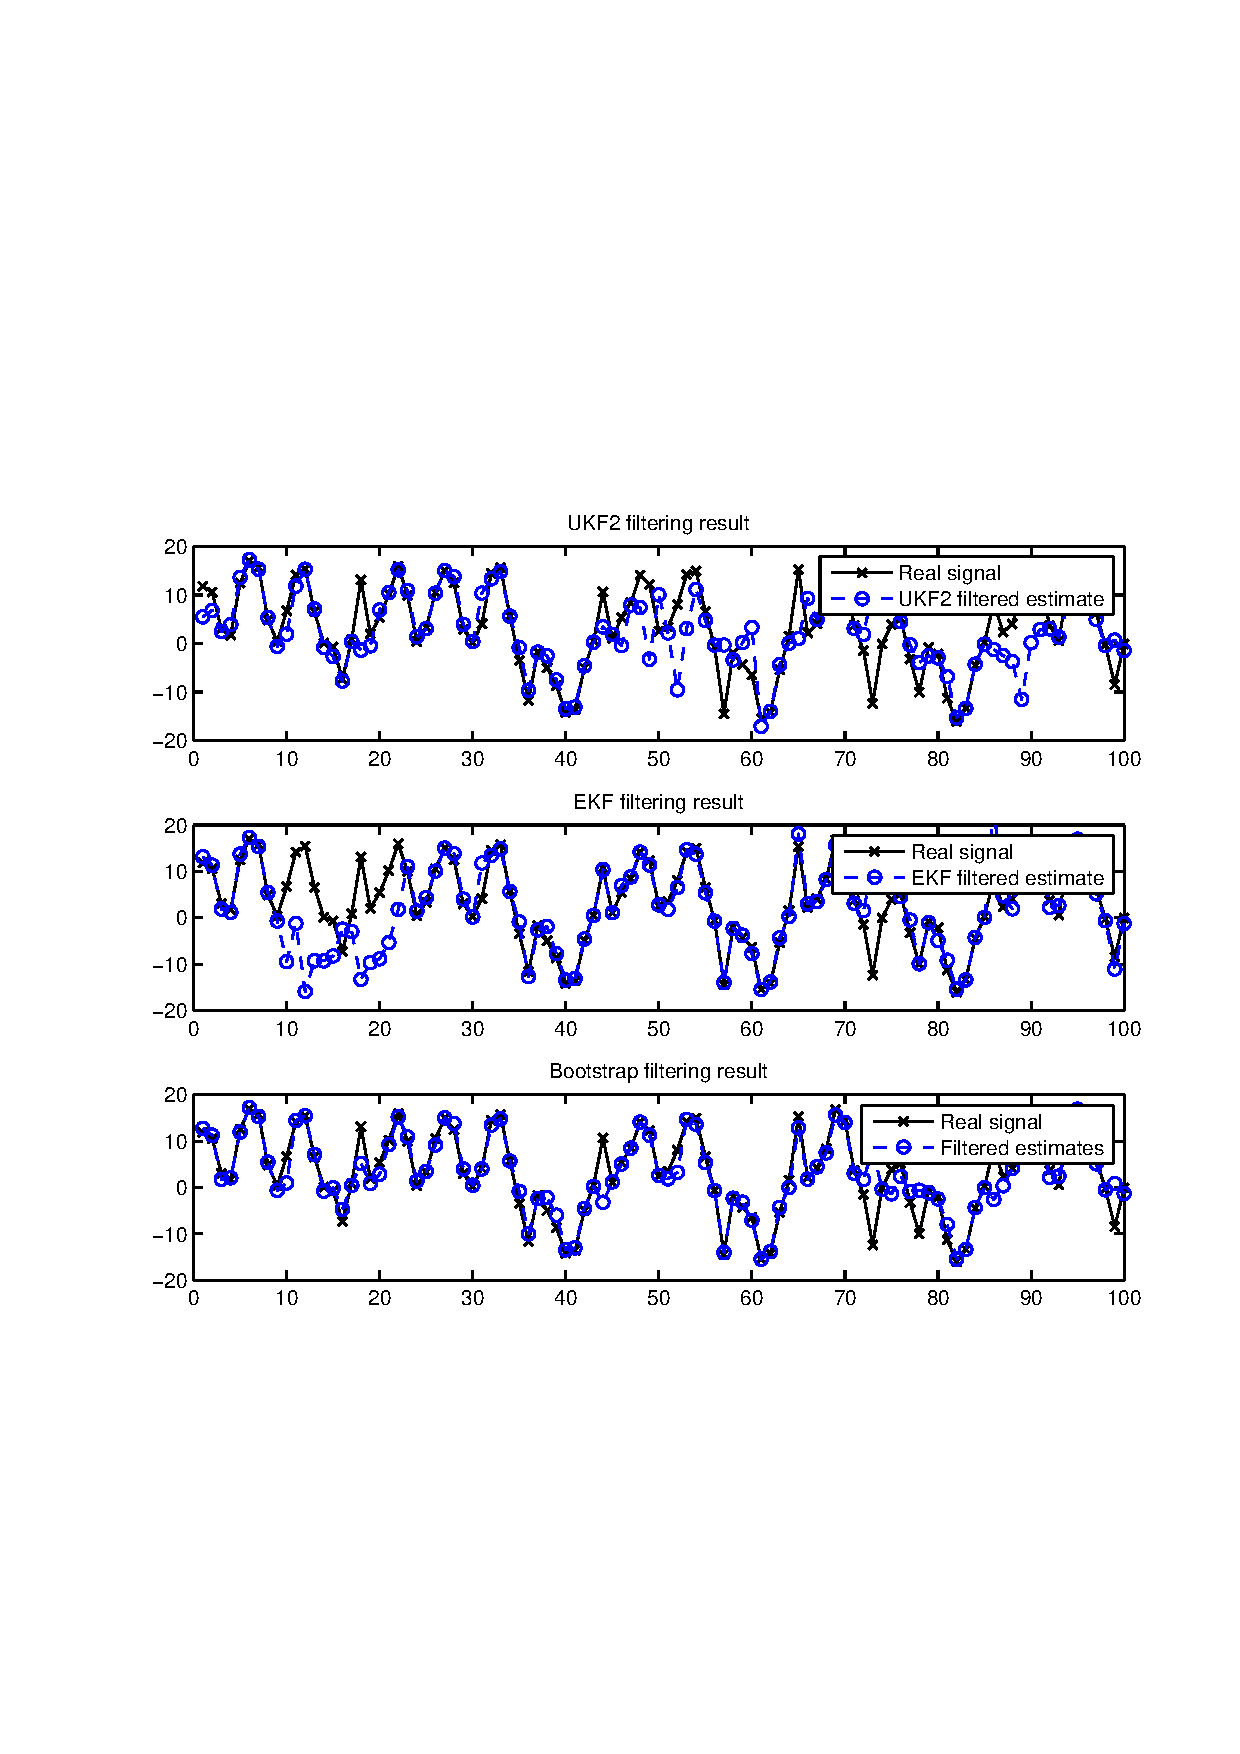
\includegraphics[width=11cm]{pics/ungm_states}
\caption{First 100 samples of filtering results of EKF, augmented form UKF and bootstrap
  filter for UNGM-model.}
\label{fig:ungm_states}
\end{center}
\end{figure}

In figure \ref{fig:ungm_c_errors} we have plotted the absolute errors
and $3\sigma$ confidence intervals of the previous figures filtering
results. It can be seen that the EKF is overoptimistic in many cases
while UKF and boostrap filter are better at telling when their
results are unreliable. Also the lower error of bootstrap filter can
be seen from the figure. The bimodality is also easy to notice on
those samples, which were mentioned above.

\begin{figure}
\begin{center}
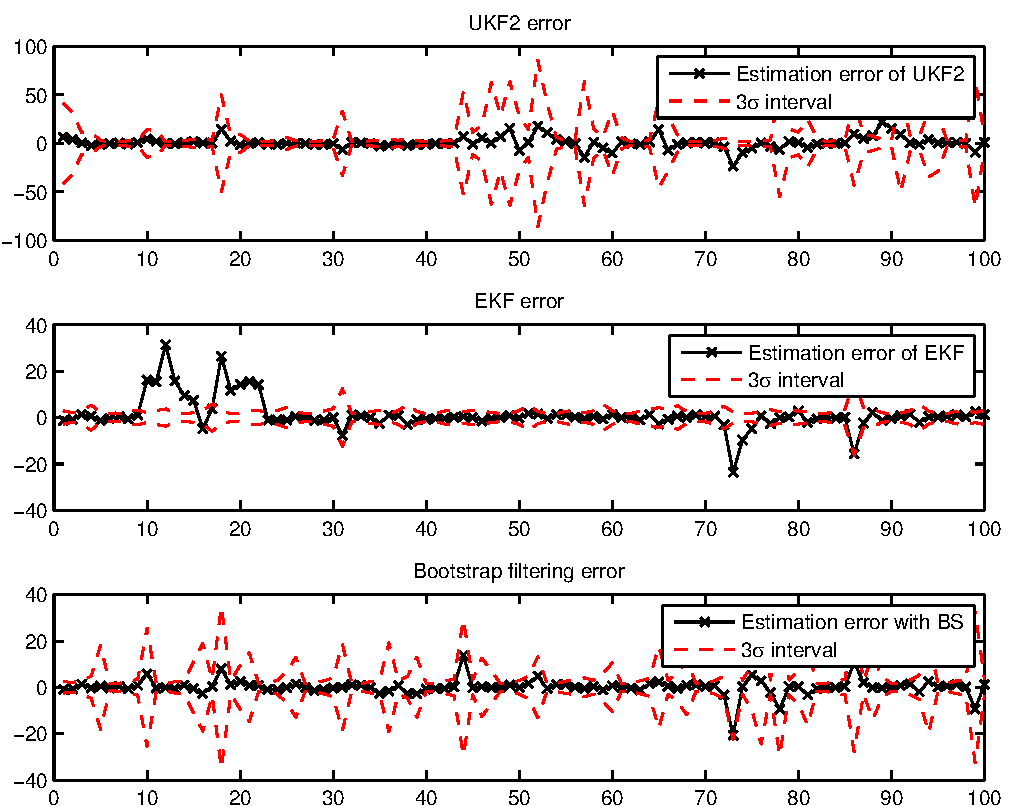
\includegraphics[width=11cm]{pics/ungm_c_errors}
\caption{Absolute errors of and $3\sigma$ confidence intervals of EKF,
  augmented form UKF and bootstrap in 100 first samples.}
\label{fig:ungm_c_errors}
\end{center}
\end{figure}

The make a comparison between nonaugmented and augmented UKF we have
plotted 100 first samples of their filtering results in figure
\ref{fig:ungm_ukf_comp}. Results are very surprising (although same as
in (Wu et al, 2005)). The reason why
nonaugmented UKF gave so bad results is not clear. However, the
better performance of augmented form UKF can be explained by the fact,
that the process noise is taken into account more effectively when the
sigma points are propagated through nonlinearity. In this case it
seems to be very crucial, as the model is highly nonlinear and multi-modal.

\begin{figure}
\begin{center}
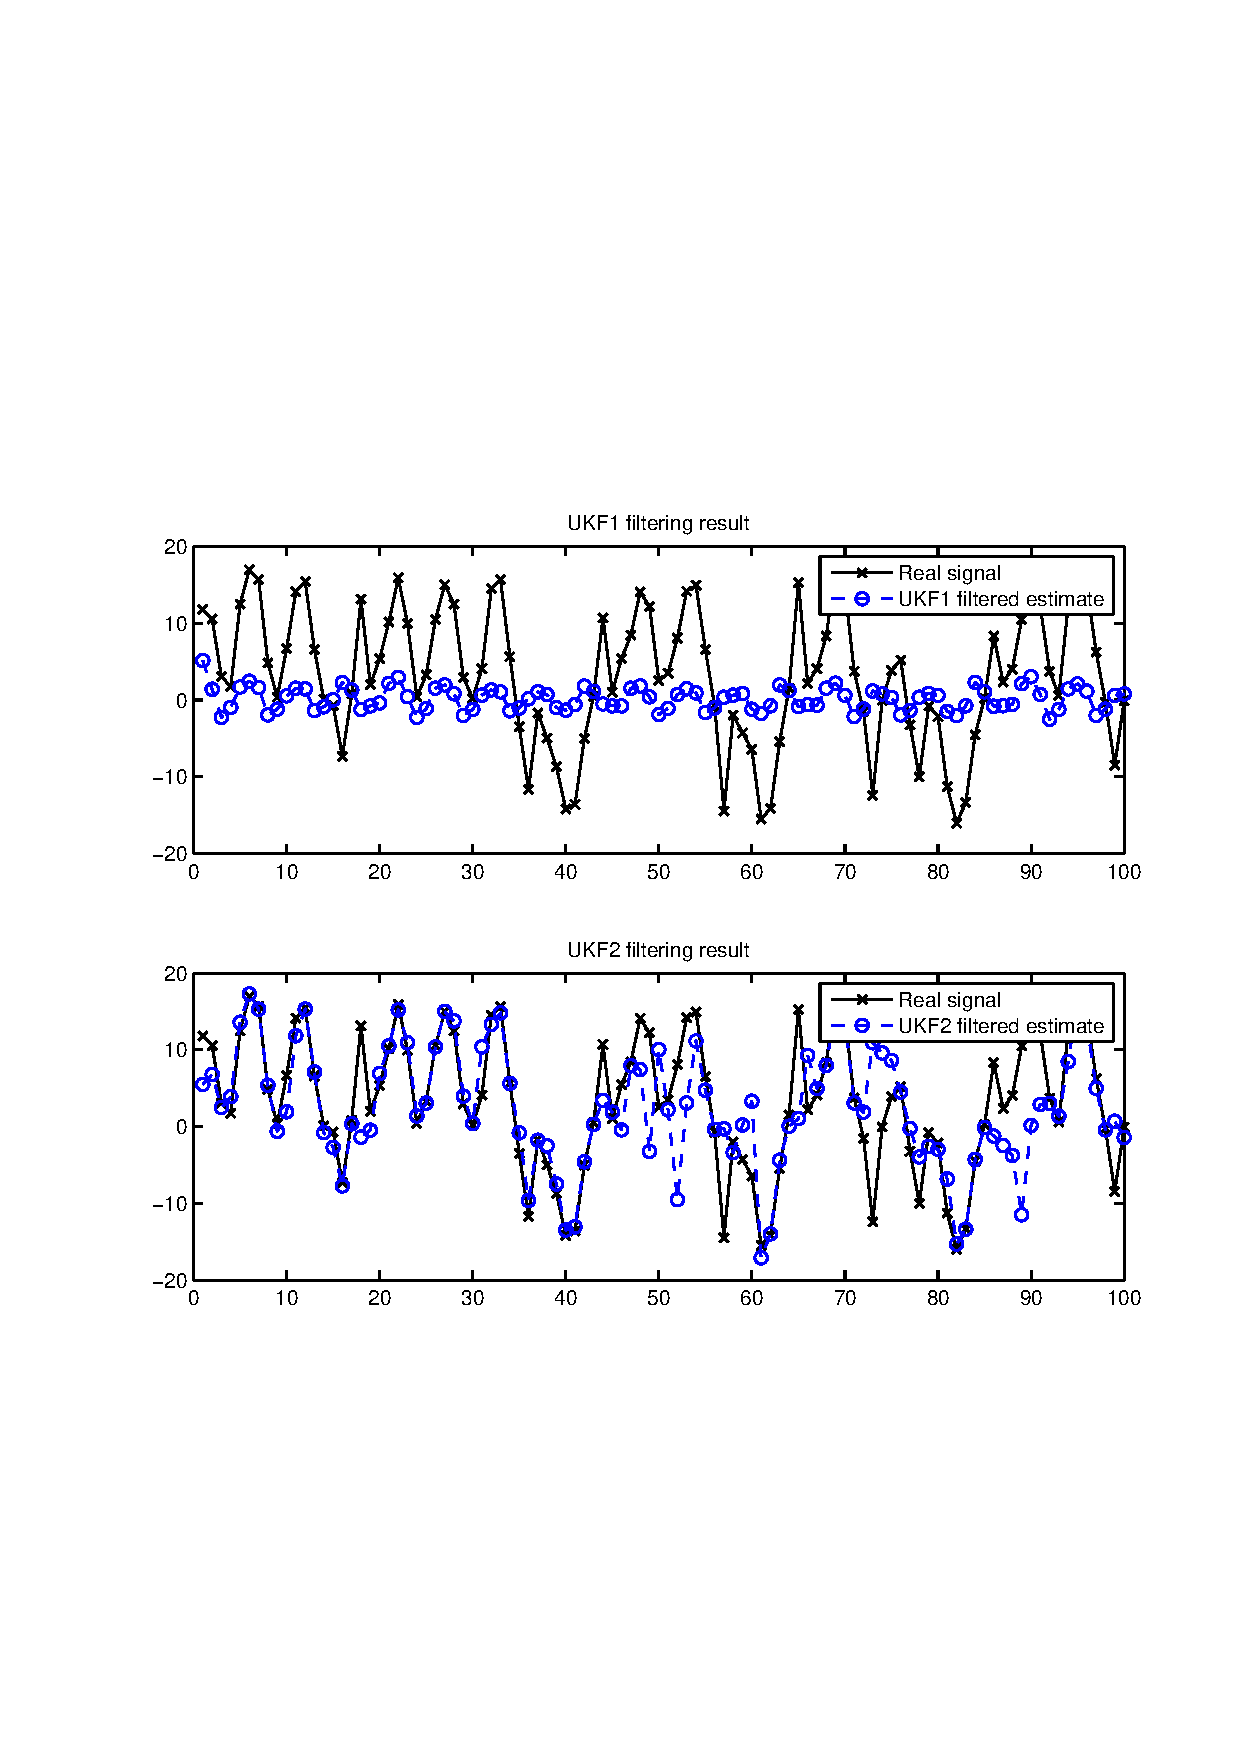
\includegraphics[width=11cm]{pics/ungm_ukf_comp}
\caption{Filtering results of nonaugmented UKF (UKF1) and augmented
  UKF (UKF2) of 100 first samples.}
\label{fig:ungm_ukf_comp}
\end{center}
\end{figure}

Lastly in figure \ref{fig:ungm_mse} we have plotted the mean square errors of each tested methods
of 100 Monte Carlo runs. Average of those errors are listed in table
\ref{table:ungm_errors}. Here is a discussion for the results:
%
\begin{itemize}
\item It is surprising that the unaugmented UKF seems to be better
  than EKF, while in above figures we have shown, that the nonaugmented UKF gives very bad
results. Reason for this is simple: the variance of the actual signal
is approximately 100, which means that by simply guessing zero
we get better performance than with EKF, on average. The
estimates of nonaugmented UKF didn't variate much on average, so they were
better than those of EKF, which on the other hand variated greatly and
gave huge errors in some cases. Because of this neither of the methods
should be used for this problem, but if one has to choose between the
two, that would be EKF, because in some cases it still gave (more or
less) right answers, whereas UKF were practically always wrong.
\item The second order EKF were also tested, but that diverged almost
  instantly, so it were left out from comparison.
\item Augmented form UKF gave clearly the best
  performance from the tested Kalman filters. As discussed above, this
  is most likely due to the fact that the process noise terms are propagated
  through the nonlinearity, and hence odd-order moment information is
  used to obtain more accurate estimates. The usage of RTS smoother seemed
  to improve the estimates in general, but oddly in some cases it made
  the estimates worse. This is most likely due to the multi-modality of
  the filtering problem.
\item Bootstrap filtering solution was clearly superior over all other
  tested methods. The result had been even better, if greater
  amount of particles had been used.
\end{itemize}

The reason why Kalman filters didn't work that well
in this case is because Gaussian approximations do not in general
apply well for multi-modal cases. Thus, a particle filtering solution
should be preferred over Kalman filters in such cases. However,
usually the particle filters need a fairly large amount of particles to be
effective, so they are generally more demanding in terms of computational
power than Kalman filters, which can be a limiting factor in real
world applications. The errors, even with bootstrap filter, were also
relatively large, so one must be careful when using the estimates
in, for example, making financial decisions. In practice this means
that one has to monitor the filter's covariance estimate, and trust the
state estimates and predictions only when the covariance estimates are
low enough, but even then there is a change, that the filter's
estimate is completely wrong.  


\begin{figure}
\begin{center}
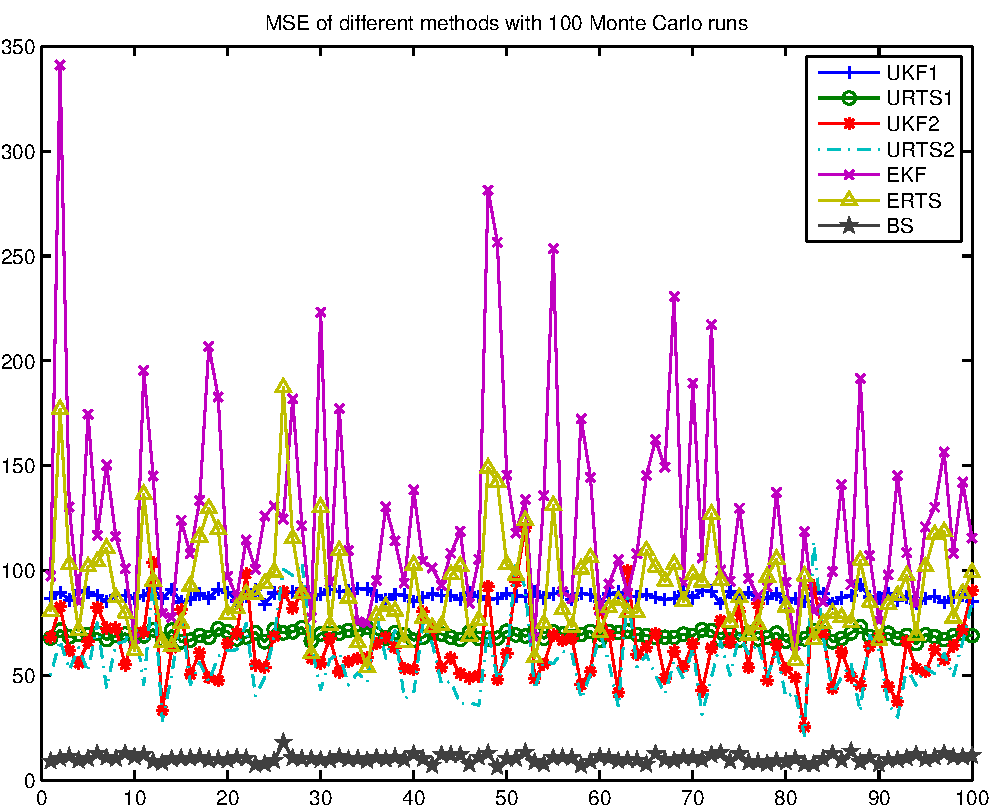
\includegraphics[width=11cm]{pics/ungm_mse}
\caption{MSEs of different methods in 100 Monte Carlo runs.}
\label{fig:ungm_mse}
\end{center}
\end{figure}

\begin{table}
\begin{center}
\begin{tabular}{|l|l|}
\hline
{\it Method}&{\it MSE[$x$]}\\
\hline
UKF1 & 87.9 \\
URTS1& 69.09 \\
UKF2  & 63.7 \\
URTS2 & 57.7 \\ 
EKF  & 125.9 \\ 
ERTS & 92.2 \\
BS   & 10.2 \\
\hline   
\end{tabular}
\caption{MSEs of estimating the UNGM model over 100 Monte Carlo simulations.}
\label{table:ungm_errors}
\end{center}
\end{table} 
 
\subsubsection{Demonstration: Bearings Only Tracking}

Next we review a classical filtering application (see, e.g.,
Bar-Shalom et al., 2001), in which we track a moving object 
with sensors, which measure only the bearings (or angles) of the
object with respect positions of the sensors. There is a one moving
target in the scene and two angular sensors for tracking it. Solving
this problem is important, because often more general multiple target
tracking problems can be partitioned into sub-problems, in which
single targets are tracked separately at a time (S�rkk�, 2006b). 

The state of the target at time step $k$ consists of the position in
two dimensional cartesian coordinates $x_k$ and $y_k$ and the velocity
toward those coordinate axes, $\dot{x}_k$ and $\dot{y}_k$. Thus,
the state vector can be expressed as 
%
\begin{equation}
%
\vec{x}_k = 
\begin{pmatrix}
x_k & y_k & \dot{x}_k & \dot{y}_k 
\end{pmatrix}^T.
%
\end{equation}
%
The dynamics of the target is modelled as a linear, discretized Wiener
velocity model (Bar-Shalom et al., 2001) 
%
\begin{equation}
%
\vec{x}_k = \begin{pmatrix}
1 & 0 & \dt & 0   \\
0 & 1 & 0   & \dt \\
0 & 0 & 1   & 0   \\
0 & 0 & 0   & 1  
\end{pmatrix}
% * 
\begin{pmatrix}
x_{k-1} \\
y_{k-1} \\
\dot{x}_{k-1} \\
\dot{y}_{k-1}    
\end{pmatrix}
+
\vec{q}_{k-1},
%
\end{equation}
% 
where $\vec{q}_{k-1}$ is Gaussian process noise with zero mean and
covariance
%
\begin{equation}
\begin{split}
E[\vec{q}_{k-1}\vec{q}^T_{k-1}] = \begin{pmatrix}
\frac{1}{3}\dt^3 & 0                 & \frac{1}{2}\dt^2 & 0 \\
0                &  \frac{1}{3}\dt^3 & 0                & \frac{1}{2}\dt^2 \\
\frac{1}{2}\dt^2 & 0                 & \dt              & 0 \\
0                & \frac{1}{2}\dt^2  & 0                & \dt  
\end{pmatrix} \\
\end{split}q,
\end{equation}
%
where $q$ is the spectral density of the noise, which is set to
$q=0.1$ in the simulations. The measurement model for sensor $i$ is defined as
%
\begin{equation}
%
\theta^i_k = \arctan \left( \frac{y_k - s^i_y}{x_k - s^i_x}\right) + r^i_k,
%
\end{equation}
%
where $(s^i_x,s^i_y)$ is the position of sensor $i$ and $r^i_k \sim
N(0,\sigma^2)$, with $\sigma = 0.05$ radians. In figure
\ref{fig:bot_measurements} we have plotted a one realization of
measurements in radians obtained from both sensors. The sensors are
placed to $(s^1_x,s^1_y) = (-1,-2)$ and $(s^2_x,s^2_y) = (1,1)$.
%
\begin{figure}
\begin{center}
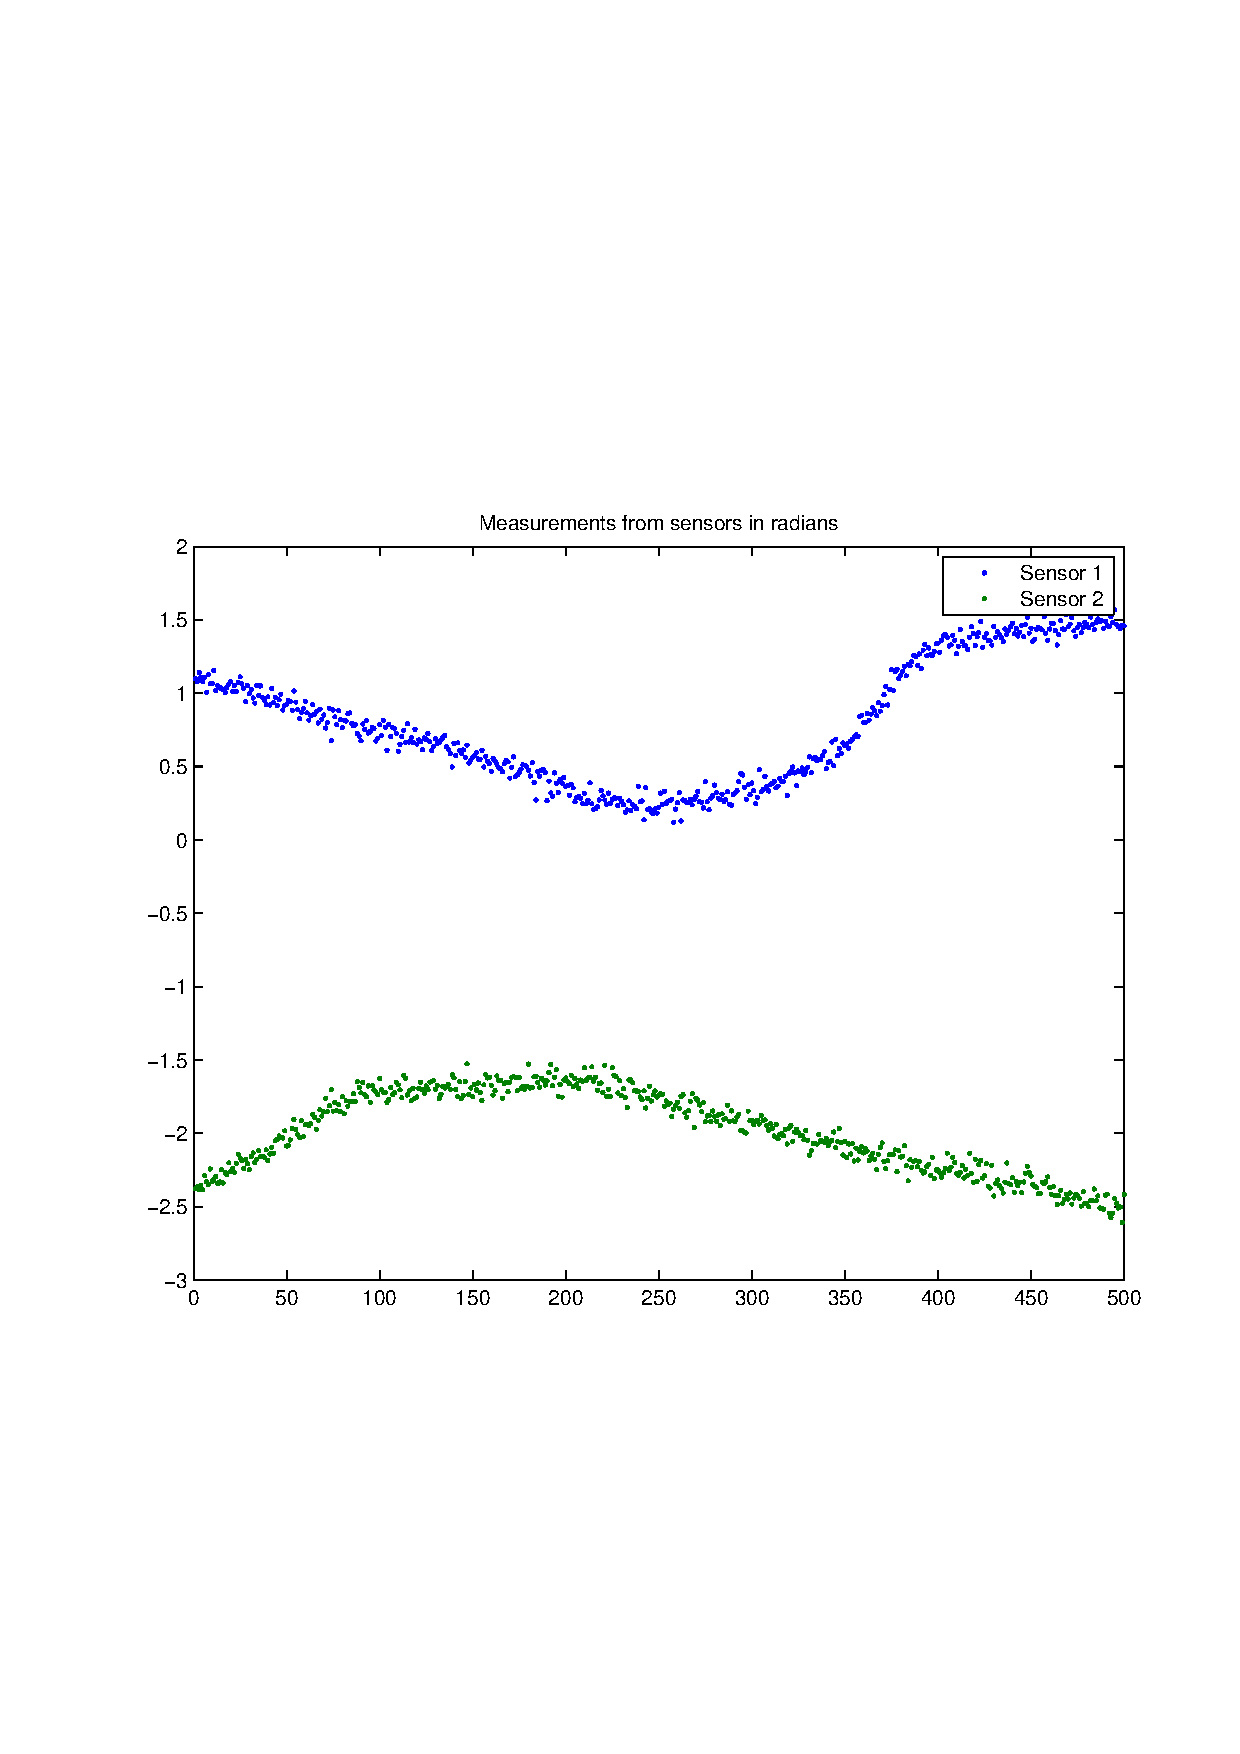
\includegraphics[width=11cm]{pics/bot_demo_measurements}
\caption{Measurements from sensors (in radians) in bearings only
  tracking problem .}
\label{fig:bot_measurements}
\end{center}
\end{figure}

The derivatives of the
measurement model, which are needed by EKF, can be computed as
%
\begin{equation}
\begin{split}
\frac{\partial \vec{h}^i(\vec{x}_k)}{\partial x_k} & = \frac{-(y_k-s^i_y)}{(x_k-s^i_x)^2+(y_k-s^i_y)^2} \\
\frac{\partial \vec{h}^i(\vec{x}_k)}{\partial y_k} & = \frac{(x_k-s^i_x)}{(x_k-s^i_x)^2+(y_k-s^i_y)^2} \\
\frac{\partial \vec{h}^i(\vec{x}_k)}{\partial \dot{x}_k} & = 0 \\
\frac{\partial \vec{h}^i(\vec{x}_k)}{\partial \dot{y}_k} & = 0 , i = 1,2.
\end{split}
\label{eq:bot_dx}
\end{equation}
%
With these the Jacobian can written as
%
\begin{equation}
\mat{H}_\vec{x}(\vec{x}_k,k) =  \begin{pmatrix}
\frac{(x_k-s^1_x)}{(x_k-s^1_x)^2+(y_k-s^1_y)^2} & \frac{-(y_k-s^1_y)}{(x_k-s^1_x)^2+(y_k-s^1_y)^2} & 0 & 0 \\
\frac{(x_k-s^2_x)}{(x_k-s^2_x)^2+(y_k-s^2_y)^2} & \frac{-(y_k-s^2_y)}{(x_k-s^2_x)^2+(y_k-s^2_y)^2} & 0 & 0   
\end{pmatrix}.
\end{equation}
%
The non-zero second order derivatives of the measurement function are also
relatively easy to compute in this model:
%
\begin{equation}
\begin{split}
\frac{\partial^2 \vec{h}^i(\vec{x}_k)}{\partial x_k \partial x_k} & = \frac{-2(x_k-s^i_x)}{((x_k-s^i_x)^2+(y_k-s^i_y)^2)^2} \\
\frac{\partial^2 \vec{h}^i(\vec{x}_k)}{\partial x_k \partial y_k} & = \frac{(y_k-s^i_y)^2-(x_k-s^i_x)^2}{((x_k-s^i_x)^2+(y_k-s^i_y)^2)^2} \\
\frac{\partial^2 \vec{h}^i(\vec{x}_k)}{\partial y_k \partial y_k} & = \frac{-2(y_k-s^i_y)}{((x_k-s^i_x)^2+(y_k-s^i_y)^2)^2}.
\end{split}
\end{equation}
%
Thus, the Hessian matrices can be written as
%
\begin{equation}
\mat{H}^i_\vec{xx}(\vec{x}_k,k) = \begin{pmatrix}
 \frac{-2(x_k-s^i_x)}{((x_k-s^i_x)^2+(y_k-s^i_y)^2)^2} &
   \frac{(y_k-s^i_y)^2-(x_k-s^i_x)^2}{((x_k-s^i_x)^2+(y_k-s^i_y)^2)^2}
   & 0 & 0 \\
 \frac{(y_k-s^i_y)^2-(x_k-s^i_x)^2}{((x_k-s^i_x)^2+(y_k-s^i_y)^2)^2} & \frac{-2(y_k-s^i_y)}{((x_k-s^i_x)^2+(y_k-s^i_y)^2)^2} & 0 & 0 \\
0 & 0 & 0 & 0 \\
0 & 0 & 0 & 0  
\end{pmatrix}, i=1,2.
\end{equation}
%
We do not list the program code for the measurement function and it's
derivatives here as they are straightforward to implement, if the
previous examples have been read.

The target starts with state $\vec{x}_0 = \begin{pmatrix} 0 & 0 & 1 & 0
\end{pmatrix}$, and in the estimation we set the prior distribution
for the state to $\vec{x}_0 \sim N(\vec{0},\mat{P}_0)$, where
%
\begin{equation}
%
\mat{P}_0 = \begin{pmatrix}
0.1 & 0 & 0 & 0\\
0 & 0.1 & 0 & 0\\
0 & 0 & 10 & 0\\
0 & 0 & 0 & 10
\end{pmatrix},
%
\end{equation}
%
which basically means that we are fairly certain about the target's
origin, but very uncertain about the velocity. In the simulations we also give the
target an slightly randomized acceleration, so that it achieves a
curved trajectory, which is approximately the same in different
simulations. The trajectory and estimates of it can be seen in figures
\ref{fig:bot_ekf1}, \ref{fig:bot_ekf2} and \ref{fig:bot_ukf}. As can
be seen from the figures EKF1 and UKF give almost identical
results while the estimates of EKF2 are clearly worse. Especially in
the beginning of the trajectory EKF2 has great difficulties in getting on
the right track, which is due to the relatively big uncertainty in the
starting location. After that the estimates are fairly similar. 

In table \ref{table:bot_rmse} we have listed the root mean square errors (mean
of position errors) of all
tested methods (same as in random sine signal example
on page \pageref{page:sine_rmse} with the addition of UFBF) over 1000
Monte Carlo runs. The numbers prove the previous observations, that
the EKF1 and UKF give almost identical performances. Same observations
apply also to smoothers. Had the prior distribution for the starting
velocity been more accurate the performance difference
between EKF2 and other methods would have been smaller, but still noticable.

\begin{table}
\begin{center}
\begin{tabular}{|l|l|}
\hline
{\it Method}&{\it RMSE } \\
\hline
EKF1 & 0.114 \\
ERTS1& 0.054 \\
EFBF1& 0.054 \\
EKF2 & 0.202 \\
ERTS2& 0.074 \\
EFBF2& 0.063 \\
UKF  & 0.113 \\
URTS & 0.055 \\
UFBF & 0.055 \\ 
\hline   
\end{tabular}
\caption{RMSEs of estimating the position in Bearings Only Tracking
  problem over 1000 Monte Carlo runs.}
\label{table:bot_rmse}
\end{center}
\end{table} 


%
\begin{figure}
\begin{center}
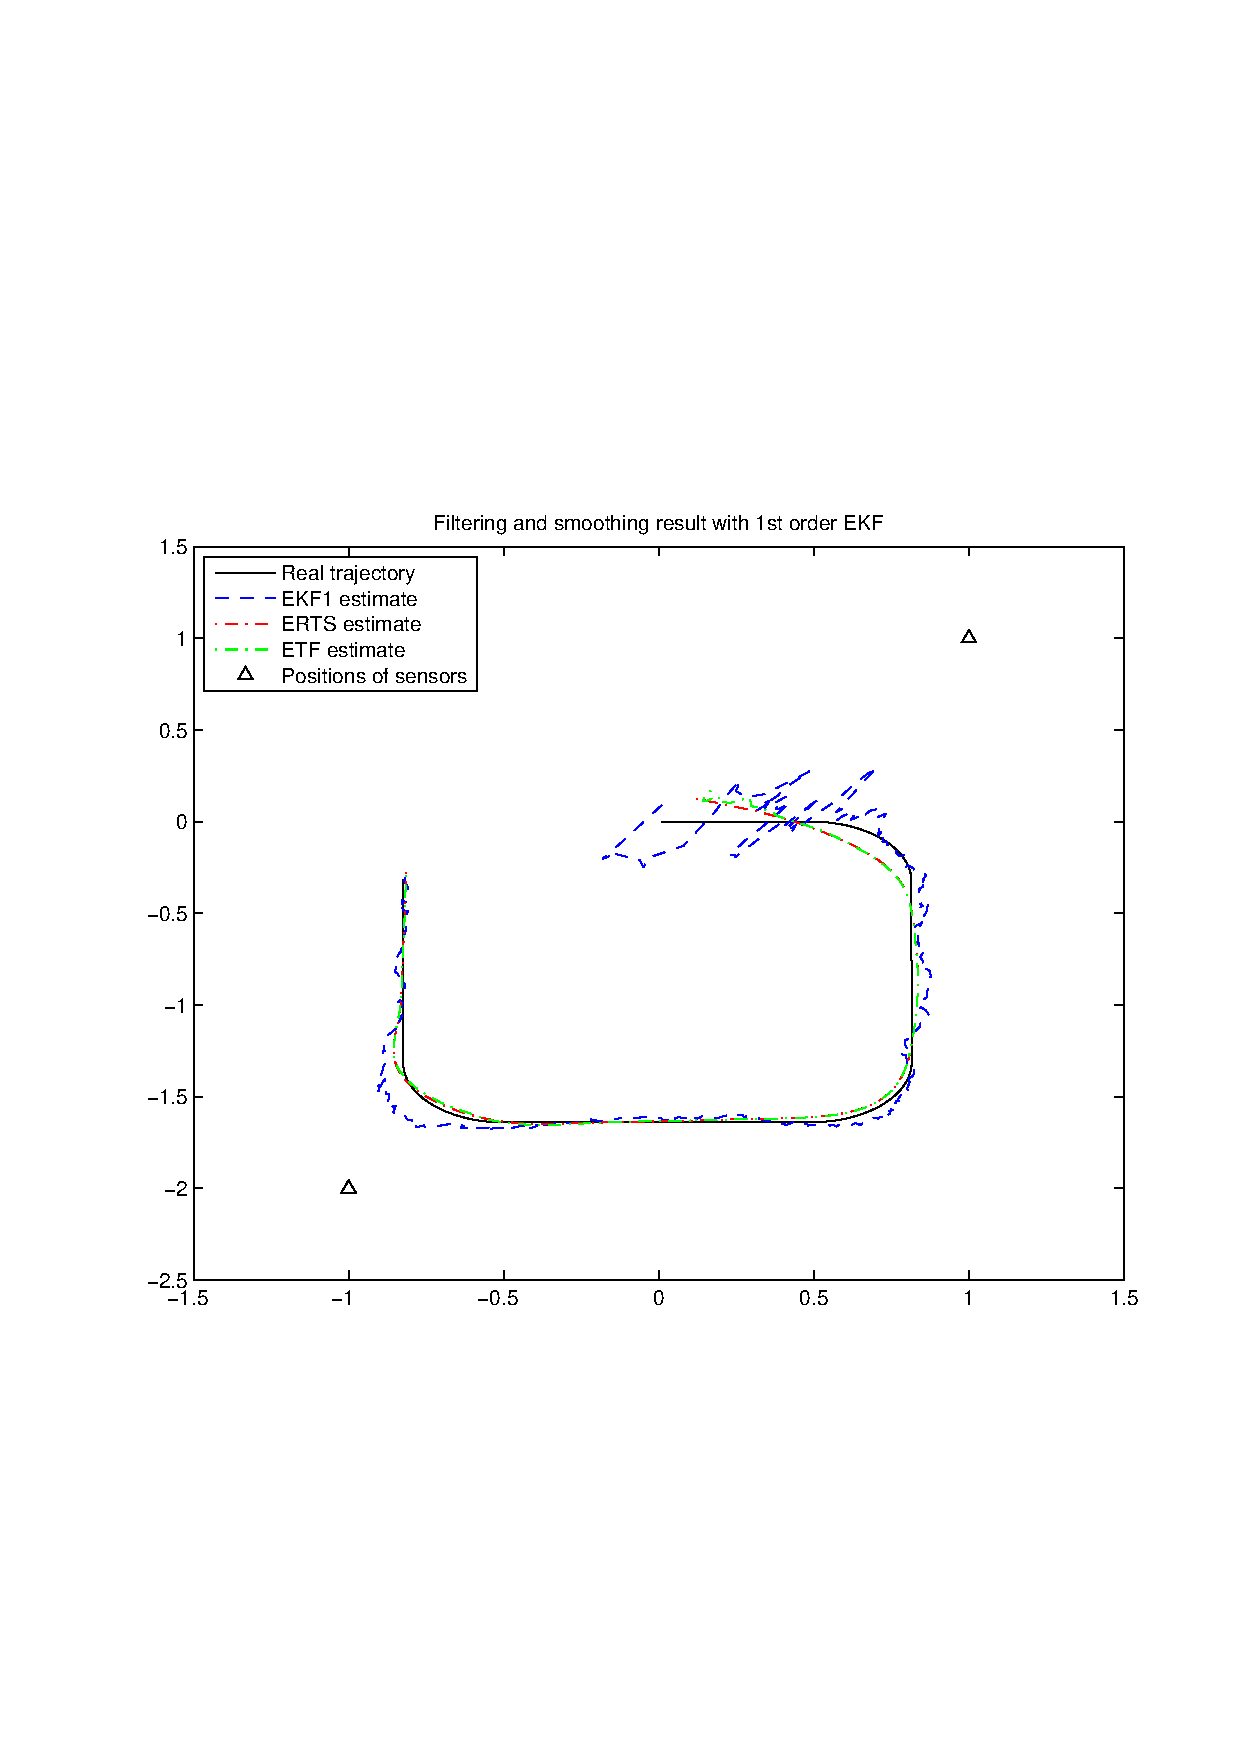
\includegraphics[width=11cm]{pics/bot_demo_ekf1}
\caption{Filtering and smoothing results of first order EKF.}
\label{fig:bot_ekf1}
\end{center}
\end{figure}

%
\begin{figure}
\begin{center}
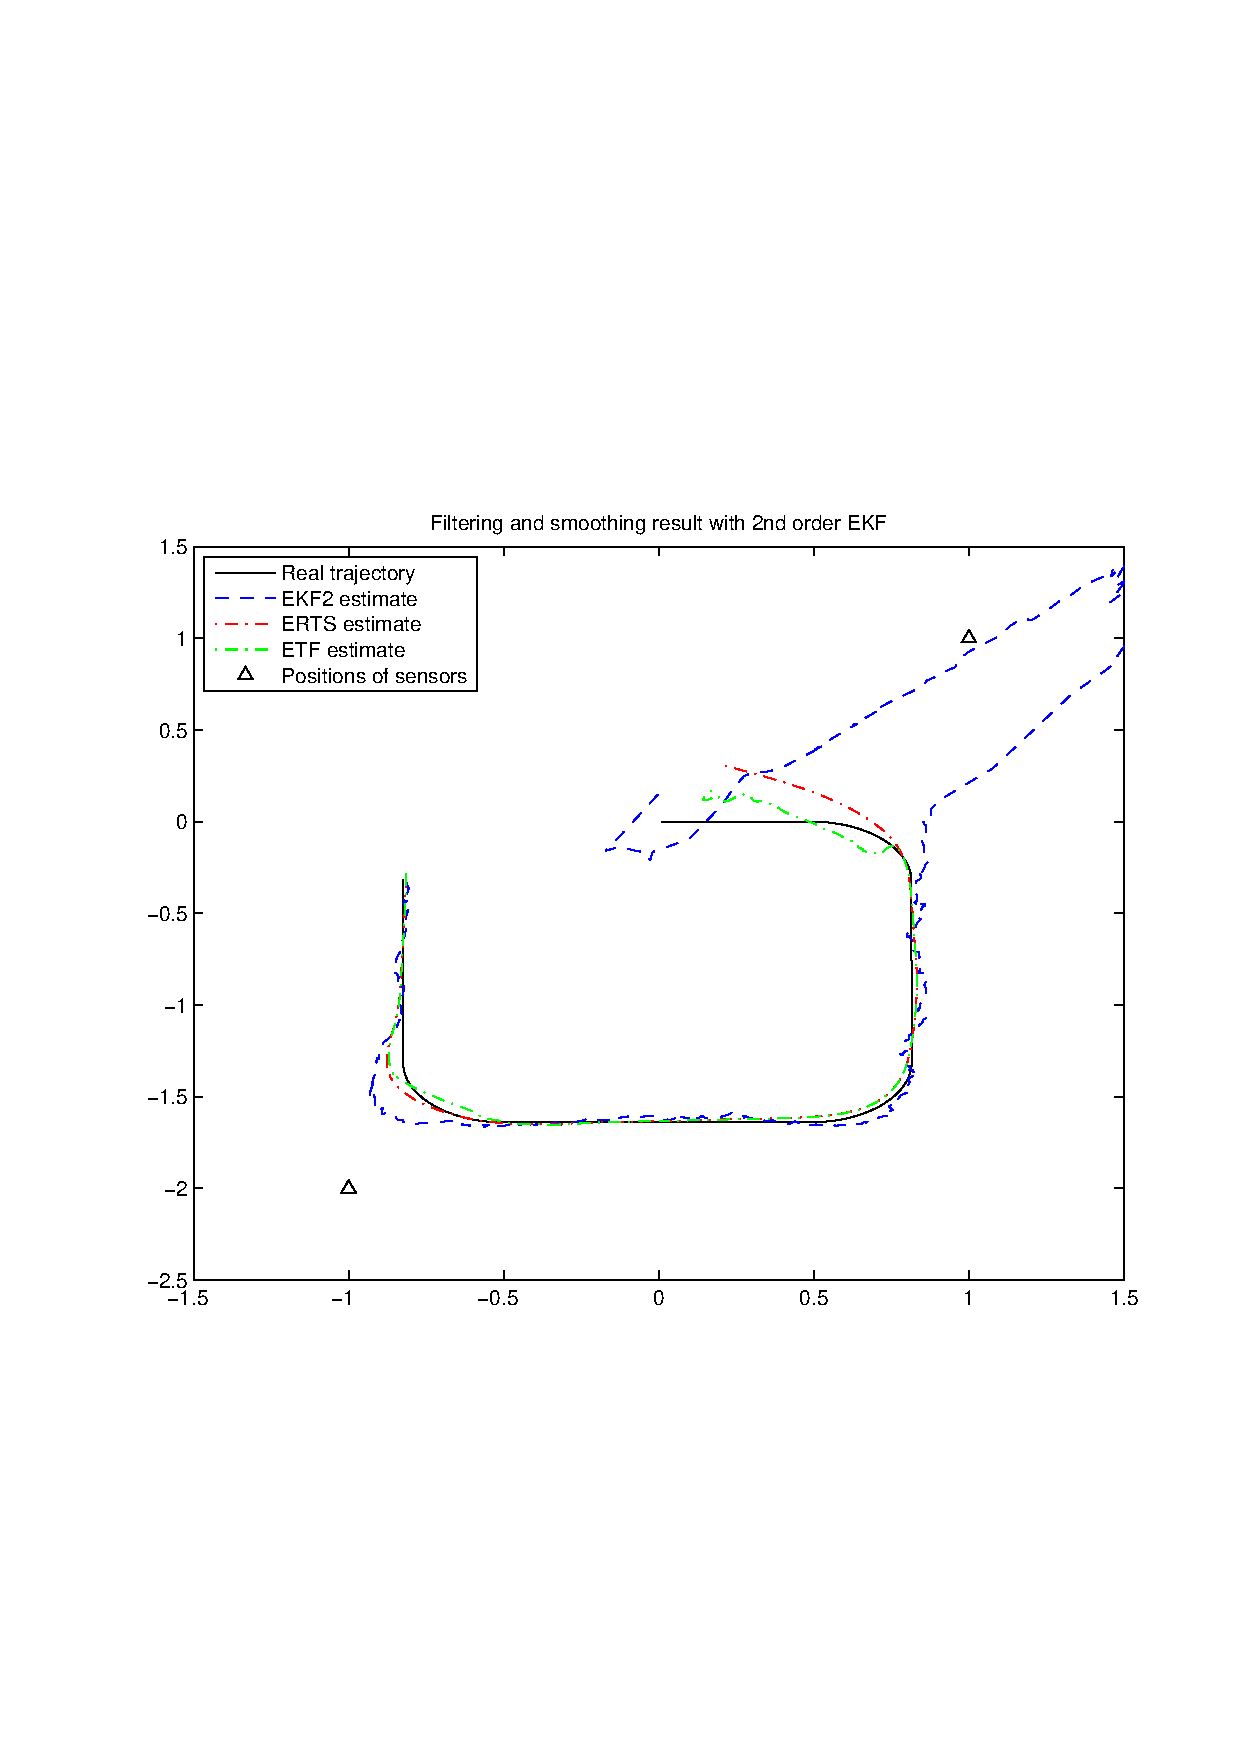
\includegraphics[width=11cm]{pics/bot_demo_ekf2}
\caption{Filtering and smoothing results of second order EKF.}
\label{fig:bot_ekf2}
\end{center}
\end{figure}

\begin{figure}
\begin{center}
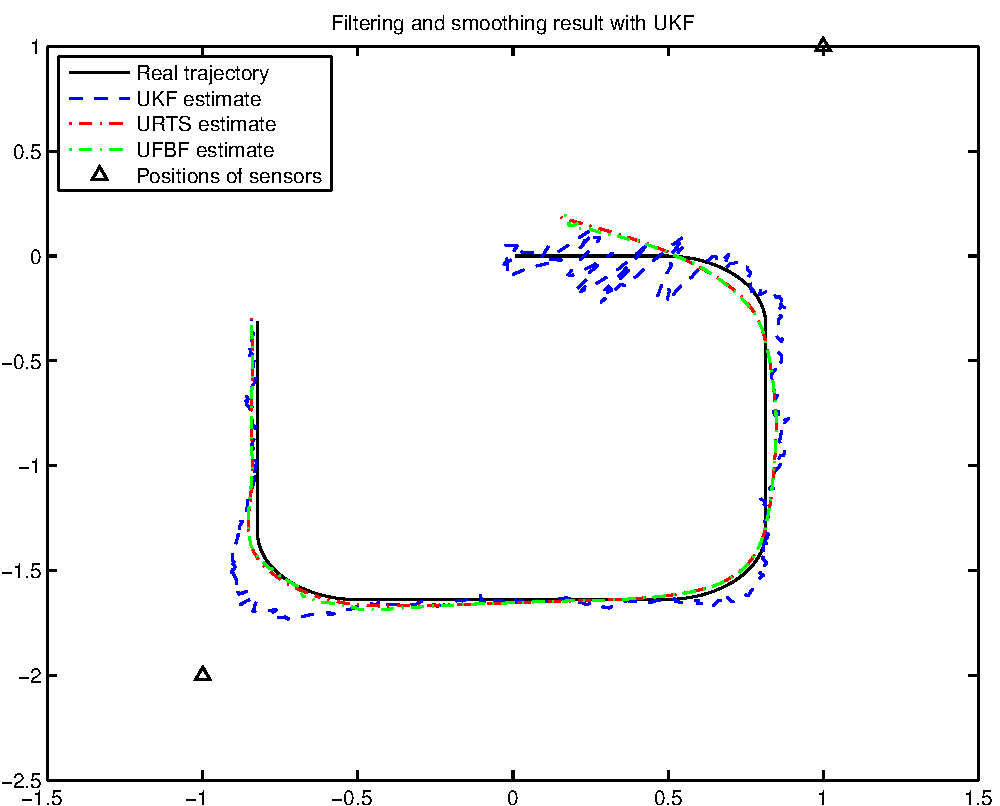
\includegraphics[width=11cm]{pics/bot_demo_ukf}
\caption{Filtering and smoothing results of UKF}
\label{fig:bot_ukf}
\end{center}
\end{figure}



\subsubsection{Demonstration: Reentry Vehicle Tracking}

As a last example we review a challenging filtering problem, which was
used in (Julier and Uhlmann, 2004b) to demonstrate the
performance of UKF. Later they released few corrections to the
model specifications and simulation parameters in (Julier and Uhlmann,
2004a). 

This example conserns a reentry tracking problem, where radar
is used for tracking a space vehicle, which enters the atmosphere at
high altitude and very high speed. Figure \ref{fig:reentry_traj} shows
a sample trajectory of the vehicle with respect to earth and radar. 
The dynamics of the vehicle are affected with three kinds of forces:
aerodynamic drag, which is a
function of of vehicle speed and has highly nonlinear variations in
altitude. The second type of force is gravity, which causes the
vehicle to accelerate toward the center of the earth. The third type
of forces are random buffetting terms. The state space in this model
consists of vehicles position ($x_1$ and $x_2$), its velocity ($x_3$
and $x_4$) and a parameter of its aerodynamic properties ($x_5$).
The dynamics in continuous case are defined as (Julier and Uhlmann, 2004b)
%
\begin{equation}
\begin{split}
%
\dot{x}_1(t) & = x_3(t) \\
\dot{x}_2(t) & = x_4(t) \\
\dot{x}_3(t) & = D(t)x_3(t) + G(t)x_1(t) + v_1(t) \\
\dot{x}_4(t) & = D(t)x_4(t) + G(t)x_2(t) + v_2(t) \\
\dot{x}_5(t) & = v_3(t),
%
\end{split}
\end{equation}
%
where $\vec{w}(t)$ is the process noise vector, $D(t)$ the
drag-related force and $G(t)$ the gravity-related force.
The force terms are given by
%
\begin{equation}
\begin{split}
%
D(k) & = \beta(t) \exp \left\{ \frac{[R_0 - R(t)]}{H_0}\right\} V(t) \\
G(t) & = -\frac{Gm_0}{R^3(t)} \\
\beta (t) & = \beta_0 \exp x_5(t),
%
\end{split}
\end{equation}
%
where $R(t) = \sqrt{x_1^2(t) + x_2^2(t)}$ is the vehicle's distance from the center of the earth
and $V(t) = \sqrt{x_3^2(t) + x_4^2(t)}$ is the speed of the vehicle.
The constants in previous definition were set to
%
\begin{equation}
\begin{split}
%
\beta_0 & = -0.59783 \\
H_0 & = 13.406 \\
Gm_0 & = 3.9860 \times 10^5 \\
R_0 & = 6374.
%
\end{split}
\end{equation}
%
To keep the implementation simple the continuous-time dynamic
equations were discretized using a simple Euler integration scheme, to give
%
\begin{equation}
\begin{split}
%
x_1(k+1) & = x_1(k) + \dt x_3(k) \\
x_2(k+1) & = x_2(k) + \dt x_4(k) \\
x_3(k+1) & = x_3(k) + \dt (D(k)x_3(k) + G(k)x_1(k)) + w_1(k+1) \\
x_4(k+1) & = x_4(k) + \dt (D(k)x_4(k) + G(k)x_2(k)) + w_2(k+1) \\
x_5(k+1) & = x_5(k) + w_3(k+1),
%
\end{split}
\end{equation}
%
where the step size between time steps was set to $\dt = 0.1s$. Note that this might
be too simple approach in real world applications due to high
nonlinearities in the dynamics, so more advanced integration scheme
(such as Runge-Kutta) might be more preferable. The discrete process noise covariance in the
simulations was set to
%
\begin{equation}
%
Q(k) = \begin{pmatrix}
2.4064 \times 10^{-5} & 0 & 0 \\
0 & 2.4064 \times 10^{-5} & 0 \\
0 & 0 & 10^{-6}
\end{pmatrix}.
%
\end{equation}
%
The lower right element in the covariance was initially in (Julier and
Uhlmann, 2004b) set to zero, but later in (Julier and Uhlmann, 2004a)
changed to $10^{-6}$ to increase filter stability.


The non-zero derivatives of the discretized dynamic equations with respect to
state variables are straightforward (although rather technical) to compute:
%
\begin{equation} 
\begin{split}
%
\frac{\partial x_1(k+1)}{\partial x_1(k)} & = 1 \\
\frac{\partial x_1(k+1)}{\partial x_3(k)} & = \dt \\
\frac{\partial x_2(k+1)}{\partial x_2(k)} & = 1 \\
\frac{\partial x_2(k+1)}{\partial x_4(k)} & = \dt \\
%
\frac{\partial x_3(k+1)}{\partial x_1(k)} & = \dt * (\frac{\partial
  D(k)}{\partial x_1(k)} x_3(k) + \frac{\partial G(k)}{\partial
  x_1(k)} x_1(k) + G(k)) \\
\frac{\partial x_3(k+1)}{\partial x_2(k)} & = \dt * (\frac{\partial
  D(k)}{\partial x_2(k)} x_3(k) + \frac{\partial G(k)}{\partial
  x_2(k)} x_1(k)) \\
\frac{\partial x_3(k+1)}{\partial x_3(k)} & = \dt * (\frac{\partial
  D(k)}{\partial x_3(k)} x_3(k) + D(k)) + 1 \\
\frac{\partial x_3(k+1)}{\partial x_4(k)} & = \dt * (\frac{\partial
  D(k)}{\partial x_4(k)} x_3(k))  \\
\frac{\partial x_3(k+1)}{\partial x_4(k)} & = \dt * (\frac{\partial
  D(k)}{\partial x_5(k)} x_3(k))  \\
%
\frac{\partial x_4(k+1)}{\partial x_1(k)} & = \dt * (\frac{\partial
  D(k)}{\partial x_1(k)} x_4(k) + \frac{\partial G(k)}{\partial
  x_1(k)} x_2(k)) \\
\frac{\partial x_4(k+1)}{\partial x_2(k)} & = \dt * (\frac{\partial
  D(k)}{\partial x_2(k)} x_4(k) + \frac{\partial G(k)}{\partial
  x_2(k)} x_2(k) + G(k)) \\
\frac{\partial x_4(k+1)}{\partial x_3(k)} & = \dt * (\frac{\partial
  D(k)}{\partial x_3(k)} x_4(k)) \\
\frac{\partial x_4(k+1)}{\partial x_4(k)} & = \dt * (\frac{\partial
  D(k)}{\partial x_4(k)} x_4(k) + D(k)) + 1 \\
\frac{\partial x_4(k+1)}{\partial x_5(k)} & = \dt * (\frac{\partial
  D(k)}{\partial x_5(k)} x_4(k))  \\
\frac{\partial x_5(k+1)}{\partial x_5(k)} & = 1,
%
\end{split}
\end{equation}
%
where the (non-zero) derivatives of the force, position and velocity
related terms with respect to state variables can be computed as
%
\begin{equation}
\begin{split}
%
\frac{\partial R(k)}{\partial x_1(k)} & = x_1(k) \frac{1}{R(k)} \\
\frac{\partial R(k)}{\partial x_2(k)} & = x_2(k) \frac{1}{R(k)} \\
\frac{\partial V(k)}{\partial x_3(k)} & = x_3(k) \frac{1}{V(k)} \\
\frac{\partial V(k)}{\partial x_4(k)} & = x_4(k) \frac{1}{V(k)} \\
\frac{\partial \beta(k)}{\partial x_5(k)} & = \beta(k)\frac{1}{R(k)} \\
\frac{\partial D(k)}{\partial x_1(k)} & = -\frac{\partial
  R(k)}{\partial x_1(k)} \frac{1}{H_0} * D(k) \\
\frac{\partial D(k)}{\partial x_2(k)} & = -\frac{\partial
  R(k)}{\partial x_2(k)} \frac{1}{H_0} * D(k) \\
\frac{\partial D(k)}{\partial x_3(k)} & = \beta(k) \exp \left\{
  \frac{[R_0 - R(k)]}{H_0}\right\} \frac{\partial V(k)}{\partial x_3} \\
\frac{\partial D(k)}{\partial x_4(k)} & = \beta(k) \exp \left\{
  \frac{[R_0 - R(k)]}{H_0}\right\} \frac{\partial V(k)}{\partial x_4} \\
\frac{\partial D(k)}{\partial x_5(k)} & = \frac{\partial \beta(k)}{x_5(k)} \exp \left\{
  \frac{[R_0 - R(k)]}{H_0}\right\} V(k) \\
\frac{\partial G(k)}{\partial x_1(k)} & = \frac{3 Gm_0}{(R(k))^4}
\frac{\partial R(k)}{\partial x_1(k)} \\ 
\frac{\partial G(k)}{\partial x_2(k)} & = \frac{3 Gm_0}{(R(k))^4} \frac{\partial R(k)}{\partial x_2(k)}.
%
\end{split}
\end{equation}
%
The prior distribution for the state were set to multivariate
Gaussian, with mean and covariance (same as in (Julier and Uhlmann, 2004b))
%
\begin{equation}
\begin{split}
%
\vec{m}_0 & = \begin{pmatrix}
6500.4 \\
349.14 \\
-1.8093 \\
-6.7967 \\
0 \\
\end{pmatrix} \\
\mat{P}_0 & = \begin{pmatrix}
10^{-6} & 0 & 0 & 0 & 0 \\
0 & 10^{-6}& 0 & 0 & 0 \\
0 & 0 & 10^{-6} & 0 & 0 \\
0 & 0 & 0 & 10^{-6}& 0 \\
0 & 0 & 0 & 0 & 1
\end{pmatrix}.
%
\end{split}
\end{equation}
%
In the simulations the initial state were drawn from multivariate
Gaussian with mean and covariance
%
\begin{equation}
\begin{split}
%
\vec{m}_0 & = \begin{pmatrix}
6500.4 \\
349.14 \\
-1.8093 \\
-6.7967 \\
0.6932 \\
\end{pmatrix} \\
\mat{P}_0 & = \begin{pmatrix}
10^{-6} & 0 & 0 & 0 & 0 \\
0 & 10^{-6}& 0 & 0 & 0 \\
0 & 0 & 10^{-6} & 0 & 0 \\
0 & 0 & 0 & 10^{-6}& 0 \\
0 & 0 & 0 & 0 & 0
\end{pmatrix},
%
\end{split}
\end{equation}
%
that is, vehicle's aerodynamic properties were not known precisely beforehand. 

The radar, which is located at $(s_x, s_y) = (R_0,0)$, is used to
measure the range $r_k$ and bearing $\theta_k$ in relation to the
vehicle on time step $k$. Thus, the measurement model can be written as
%
\begin{equation}
\begin{split}
%
r_k & = \sqrt{(x_1(k) - s_x)^2 + (x_2(k) - s_y)^2} + q_1(k) \\
\theta_k & = \tan^{-1} \left( \frac{x_2(k) - s_y}{x_1(k) - s_x}\right)
+q_2(k),
%
\end{split}
\end{equation}
%
where the measurement noise processes $q_1(k)$ and $q_2(k)$ are
Gaussians with zero means and standard deviations $\sigma_{r} =
10^{-3} \text{km}$ and $\sigma_{\theta} = 0.17 \text{mrad}$,
respectively. The derivatives of $\theta_k$ with respect to state
variables can computed with equations (\ref{eq:bot_dx}). For $r_k$ the
derivatives can be written as
%
\begin{equation}
\begin{split}
\frac{\partial r_k}{\partial x_1(k)} & = x_1(k) \frac{1}{r_k} \\
\frac{\partial r_k}{\partial x_2(k)} & = x_2(k) \frac{1}{r_k}.
\end{split}
\end{equation}
%

\begin{figure}
\begin{center}
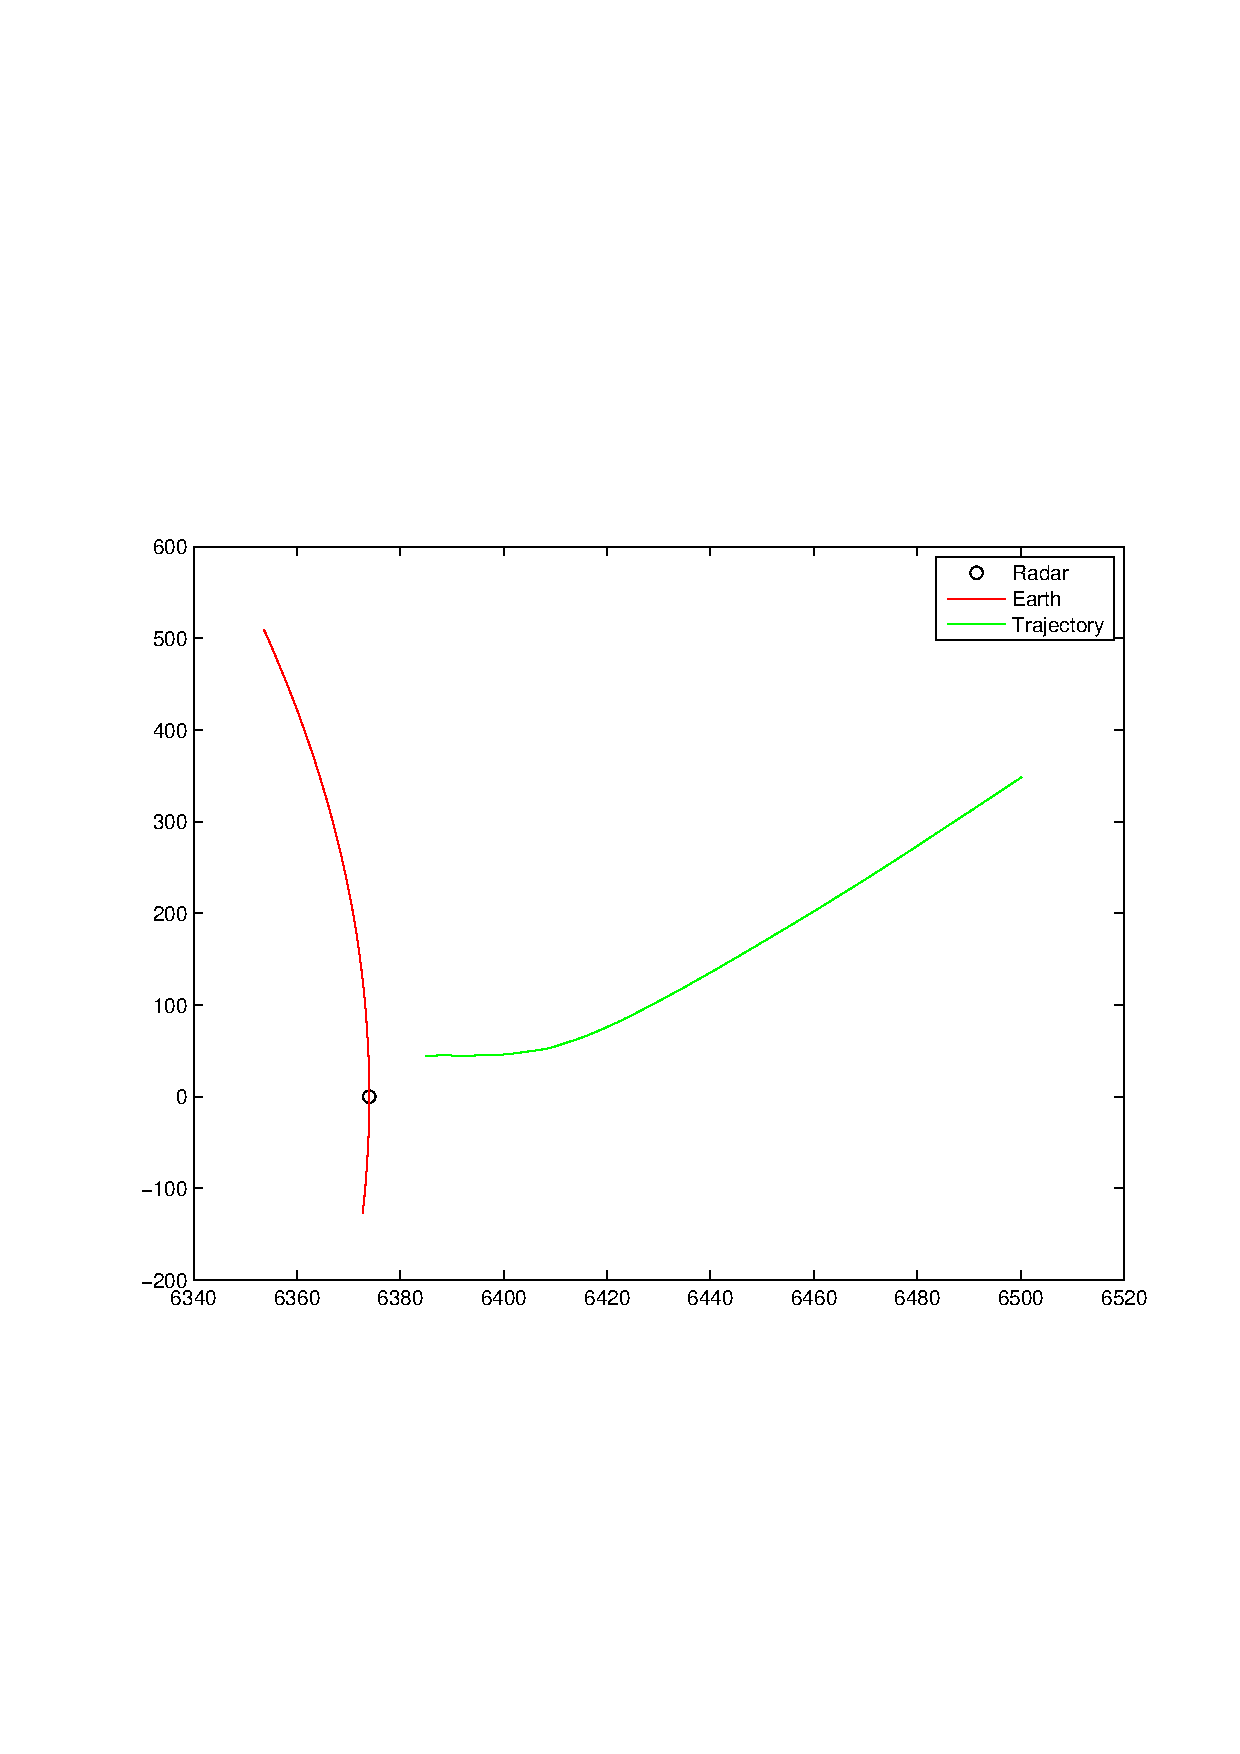
\includegraphics[width=11cm]{pics/reentry_trajectory}
\caption{Sample vehicle trajectory, earth and position of radar in
  Reentry Vehicle Tracking problem.}
\label{fig:reentry_traj}
\end{center}
\end{figure}

In the table \ref{table:reentry_rmse} we have listed the RMS errors of
position estimates with tested methods, which were
%
\begin{itemize}
%
\item EKF1: first order extended Kalman filter. 
\item ERTS: first order Rauch-Tung-Striebel smoother.
\item UKF: augmented form unscented Kalman filter.
\item URTS1: unscented Rauch-Tung-Striebel smoother with non-augmented
sigma points.
\item URTS2: unscented Rauch-Tung-Striebel smoother with augmented
sigma points.
\item UFBF: unscented Forward-Backward smoother.
%
\end{itemize}
%
Extended Forward-Backward smoother was also tested, but it produced
in many cases divergent estimates, so it were left out from
comparison. Second order EKF were also left out, because
evaluating the Hessians would have taken too much work while considering the
fact, that the estimates might have gotten even worse.  

From the error estimates we can see, that EKF and UKF
give almost identical performances, altough in the article (Julier and
Uhlmann, 2004b) UKF was clearly superior over EKF. The reason for this
might be the fact that they used numerical approximations (central
differences) for calculating the Jacobian in EKF rather than
calculating the derivatives in closed form, as was done in this demonstration. 

In figure \ref{fig:reentry_errors} we have plotted the mean square errors and
variances in estimating $x_1$, $x_3$ and $x_5$ with EKF and ERTS over 100
Monte Carlo runs. It shows that using smoother always gives better
estimates for positions and velocities, but for $x_5$ the errors are
practically the same after $\sim 45$ seconds. This also shows that both methods are pessimistic
in estimating $x_5$, because variances were bigger than the true
errors. Figures for $x_2$ and $x_4$ are not shown, because
they very similar to the ones of $x_1$ and $x_3$. Also by using UKF and URTS the
resulting figures were in practically identical, and therefore left out.
% 
%  
\begin{table}
\begin{center}
\begin{tabular}{|l|l|}
\hline
{\it Method}&{\it RMSE } \\
\hline
EKF1  & 0.0083 \\
ERTS & 0.0043 \\
UKF   & 0.0083 \\
URTS1 & 0.0043 \\
URTS2 & 0.0043 \\ 
UFBF  & 0.0044 \\
\hline 
\end{tabular}
\caption{Average RMSEs of estimating the position in Reentry Vehicle
  Tracking problem over 100 Monte Carlo runs.}
\label{table:reentry_rmse}
\end{center}
\end{table} 
%
\begin{figure}
\begin{center}
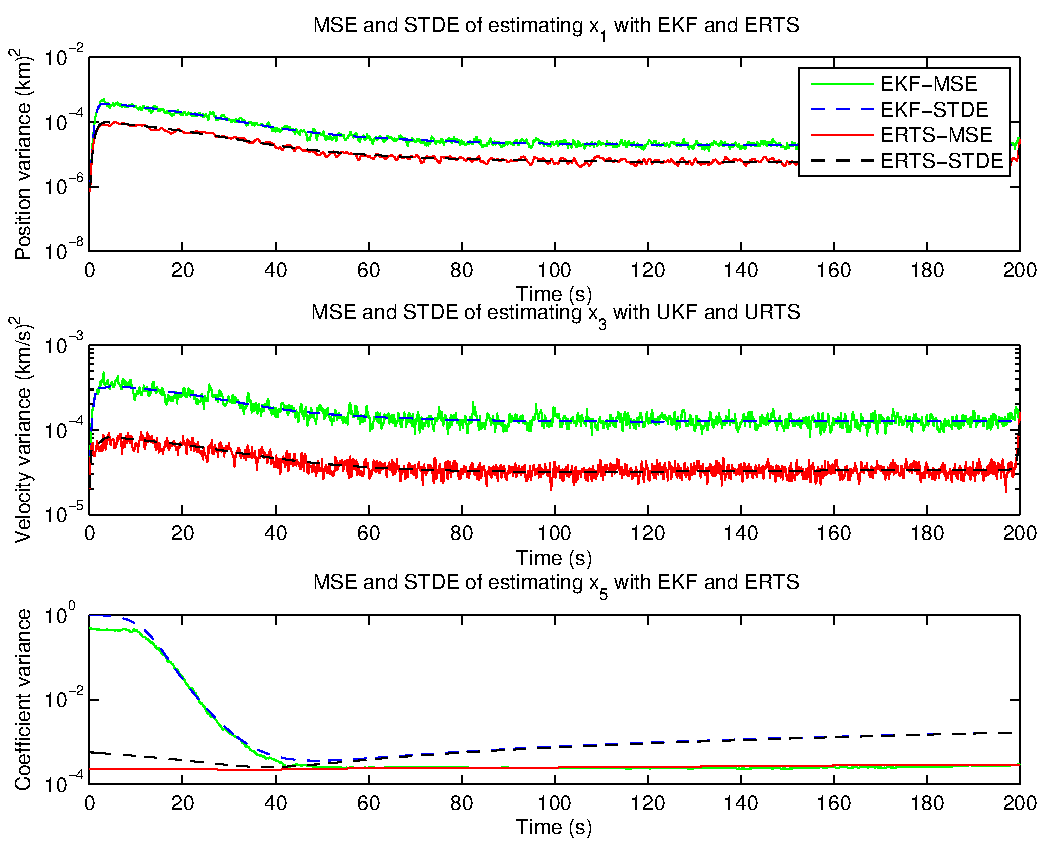
\includegraphics[width=11cm]{pics/reentry_errors}
\caption{MSEs and variances in estimating of $x_1$, $x_3$ and $x_5$ using EKF and ERTS over
  100 Monte Carlo runs.}
\label{fig:reentry_errors}
\end{center}
\end{figure}

\clearpage
%\newpage
%\newpage
%%%%%%%%%%%%%%%%%%%%%%%%%%%%%%%%%%%%%%%%%%%%%%%%%%%%%%%%%%%%%%%%%%%%%%%%%%%%%%
%
\section{Functions in the toolbox}
%
%%%%%%%%%%%%%%%%%%%%%%%%%%%%%%%%%%%%%%%%%%%%%%%%%%%%%%%%%%%%%%%%%%%%%%%%%%%%%%

In table \ref{table:functions} we have listed all the functions in the
toolbox and the page numbers (sorted by page numbers in increasing order), where
the function description begins. Some of the functions have optional
input parameters. The default values for these parameters are listed
in end of parameter descriptions.

%
\begin{table}
\begin{center}
\begin{tabular}{|r|r|}
\hline
Function & Page\\
\hline
\hline
\texttt{lti\_disc} & \pageref{page:lti_disc}\\
\hline
\texttt{kf\_predict} & \pageref{page:kf_predict}\\
\texttt{kf\_update} & \pageref{page:kf_update}\\
\texttt{rts\_smooth} & \pageref{page:rts_smooth}\\
\texttt{fbf\_smooth} & \pageref{page:fbf_smooth}\\
\hline
\texttt{ekf\_predict1} & \pageref{page:ekf_predict1}\\
\texttt{ekf\_update1} & \pageref{page:ekf_update1}\\
\texttt{ekf\_predict2} & \pageref{page:ekf_predict2}\\
\texttt{ekf\_update2} & \pageref{page:ekf_update2}\\
\texttt{erts\_smooth1} & \pageref{page:erts_smooth1}\\
\texttt{efbf\_smooth1} & \pageref{page:efbf_smooth1}\\
\hline
\texttt{ut\_weights} & \pageref{page:ut_weights}\\
\texttt{ut\_mweights} & \pageref{page:ut_mweights}\\
\texttt{ut\_sigmas} & \pageref{page:ut_sigmas}\\
\texttt{ut\_transform} & \pageref{page:ut_transform}\\
\texttt{ukf\_predict1} & \pageref{page:ukf_predict1}\\
\texttt{ukf\_update1} & \pageref{page:ukf_update1}\\
\texttt{ukf\_predict2} & \pageref{page:ukf_predict2}\\
\texttt{ukf\_update2} & \pageref{page:ukf_update1}\\
\texttt{ukf\_predict3} & \pageref{page:ukf_predict3}\\
\texttt{ukf\_update3} & \pageref{page:ukf_update1}\\
\texttt{urts\_smooth1} & \pageref{page:urts_smooth1}\\
\texttt{urts\_smooth2} & \pageref{page:urts_smooth2}\\
\texttt{ufbf\_smooth1} & \pageref{page:ufbf_smooth1}\\
\hline
\texttt{der\_check} & \pageref{page:der_check}\\
\texttt{gauss\_pdf} & \pageref{page:gauss_pdf}\\
\texttt{gauss\_rnd} & \pageref{page:gauss_rnd}\\
\texttt{rk4} & \pageref{page:rk4}\\
\texttt{schol} & \pageref{page:schol}\\
\hline
\end{tabular}
\caption{Functions provided with the toolbox. Functions are sorted
  according to page numbers, from which function descriptions begin.}
\label{table:functions}
\end{center}
\end{table}

%%%%%%%%%%%%%%%%%%%%%%%%%%%%%%%%%%%%%%%%%%%%%%%%%%%%%%%%%%%%%%%%%%%%%%%%%%%%%%
%
\subsection{Discrete-time state space estimation}
%
%%%%%%%%%%%%%%%%%%%%%%%%%%%%%%%%%%%%%%%%%%%%%%%%%%%%%%%%%%%%%%%%%%%%%%%%%%%%%%

\label{page:lti_disc}

%{\bf The discretization of a continous-time dynamic system} using the matrix fractional
%decomposition (equation (\ref{eq:noisy_ltisolution_cov1})) can be calculated with the function
%\texttt{lti\_disc}: \\

\noindent \begin{tabular}{|l|}
\hline

{\bf \texttt{lti\_disc}} \\

%{\bf Description:}
%\begin{tabular}{l}
Discretizes a linear, continous-time dynamic system using the matrix \\
fraction decomposition (eq. (\ref{eq:noisy_ltisolution_cov1})). \\
%\end{tabular} \\

\hline

{\bf Syntax:}
%
\texttt{[A,Q] = lti\_disc(F,L,Qc,dt)} \\

\hline
{\bf Input:}
%
\begin{tabular}{l l l}
\texttt{F} & $N\times N$ feedback matrix \\
\texttt{L} & $N\times L$ noise effect matrix & default: identity \\
\texttt{Qc} & $L \times L$ diagonal diffusion matrix & default: zeros \\
\texttt{dt} & time step                              & default: 1 \\
\end{tabular}\\
\hline

{\bf Output:}
%
\begin{tabular}{l l}
\texttt{A} & The transition matrix\\
\texttt{Q} & The covariance of the discrete process\\
\end{tabular}\\

\hline
\end{tabular}

%%%%%%%%%%%%%%%%%%%%%%%%%%%%%%%%%%%%%%%%%%%%%%%%%%%%%%%%%%%%%%%%%%%%%%%%%%%%%%
%
\subsubsection{Linear models}
%
%%%%%%%%%%%%%%%%%%%%%%%%%%%%%%%%%%%%%%%%%%%%%%%%%%%%%%%%%%%%%%%%%%%%%%%%%%%%%%

\subsubsection*{Kalman filter}

%{\bf The prediction step} of the Kalman filter (eq. (\ref{eq:dkf_predict}))
%can be calculated using the function \texttt{kf\_predict}:\\



\label{page:kf_predict}


\begin{tabular}{|l|}
\hline

{\bf \texttt{kf\_predict}} \\

Calculates the {\bf prediction step} of the Kalman filter (eq.
(\ref{eq:dkf_predict})). \\

\hline

{\bf Syntax:}
%
\texttt{[X,P] = kf\_predict(X,P,A,Q,B,U)} \\

\hline
{\bf Input:}
%
\begin{tabular}{l l l}
\texttt{X} & $N\times 1$ vector containing the state mean estimate of the previous step\\
\texttt{P} & $N\times N$ matrix containing the state covariance of the previous step\\
\texttt{A} & Transition matrix of the discrete model & default: identity\\
\texttt{Q} & Process noise of the discrete model & default: zero\\
\texttt{B} & Input effect matrix & default: identity\\
\texttt{U} & Constant input & default: empty\\
\end{tabular}\\
\hline

{\bf Output:}
%
\begin{tabular}{l l}
\texttt{X} & Predicted mean for the state on the next time step\\
\texttt{P} & Predicted covariance for the state on the next time step\\
\end{tabular}\\

\hline
\end{tabular}

%\noindent {\bf The update step} of the Kalman filter (eq. \ref{eq:dkf_update}) can
%be calculated using the function \texttt{kf\_update}: \\

\label{page:kf_update}

\noindent \begin{tabular}{|l|}
\hline

{\bf \texttt{kf\_update}} \\

Calculates the {\bf update step} of the Kalman filter (eq.
\ref{eq:dkf_update}). \\

\hline

{\bf Syntax:}
\texttt{[X,P,K,IM,IS,LH] = kf\_update(X,P,Y,H,R)} \\

\hline
{\bf Input:}
%
\begin{tabular}{l l}
\texttt{X} & $N\times 1$ vector containing the predicted state mean estimate from the prediction step\\
\texttt{P} & $N\times N$ matrix containing the predicted state covariance of the prediction step\\
\texttt{Y} & $D\times 1$ vector containing the measurement on this time step\\
\texttt{H} & $N\times D$ measurement matrix on this time step\\
\texttt{R} & $S\times D$ measurement noise covariance matrix on this time step\\
\end{tabular}\\
\hline

{\bf Output:}
%
\begin{tabular}{l l}
\texttt{X}  & $N\times 1$ vector containing the updated state mean\\
\texttt{P}  & $N\times N$ matrix containing the updated state covariance\\
\texttt{K}  & Computed gain for the Kalman filter\\
\texttt{IM} & Mean of predictive distribution of \texttt{Y}\\
\texttt{IS} & Covariance or predictive mean of \texttt{Y}\\
\texttt{LH} & Predictive probability of the measurement\\
\end{tabular}\\

\hline


\end{tabular}
\subsubsection*{Kalman smoother}


%{\bf The smoothed estimate} for the state mean and covariance using {\bf the RTS smoother}
%(eq. (\ref{eq:kfrts})) can be calculated with function \texttt{rts\_smooth}:\\

\label{page:rts_smooth}

\begin{tabular}{|l|}
\hline

{\bf \texttt{rts\_smooth}} \\

Computes {\bf The smoothed estimate} for the state mean and covariance using {\bf the RTS smoother}
(eq. (\ref{eq:kfrts})).\\

\hline
{\bf Syntax:} 
\texttt{[M,P,S] = rts\_smooth(M,P,A,Q)} \\

\hline
{\bf Input:}
%
\begin{tabular}{l l}
\texttt{M} & $N\times K$ matrix containing $K$ mean estimates calculated with Kalman filter\\
\texttt{P} & $N\times N\times K$ matrix of $K$ state covariances calculated with Kalman filter \\
\texttt{A} & $N\times N$ state transition matrix or $N\times N\times K$ matrix of $K$ state covariances
\\ & for each time step\\
\texttt{Q} & $N\times N$ process noise covariance matrix or $N\times N\times K$ matrix of $K$ process\\ & noise covariance matrices for each time step
\end{tabular}\\
\hline

{\bf Output:}
%
\begin{tabular}{l l}
\texttt{M} & Smoothed state mean on each time step\\
\texttt{P} & Smoothed state covariance sequence on each time step\\
\texttt{S} & Smoother gain on each time step
\end{tabular}\\

\hline
\end{tabular}

%{\bf The smoothed estimate} for the state mean and covariance using {\bf the FBF smoother}
%can be calculated with function \texttt{fbf\_smooth}:\\

\label{page:fbf_smooth}

\noindent \begin{tabular}{|l|}
\hline

{\bf \texttt{fbf\_smooth}} \\

Calculates the {\bf The smoothed estimate} for the state mean and covariance using {\bf the FBF smoother}.\\

\hline

{\bf Syntax:} 
\texttt{[M,P] = fbf\_smooth(M,P,Y,A,Q,H,R,use\_inf)} \\

\hline
{\bf Input:}
%
\begin{tabular}{l l}
\texttt{M} & $N\times K$ matrix containing $K$ mean estimates calculated with Kalman filter\\
\texttt{P} & $N\times N\times K$ matrix of $K$ state covariances calculated with Kalman filter \\
\texttt{Y} & $D\times K$ matrix containing the sequence of $K$ measurements \\
\texttt{A} & $N\times N$ state transition matrix or $N\times N\times K$ matrix of $K$ state covariances
\\ & for each time step\\
\texttt{Q} & $N\times N$ process noise covariance matrix or $N\times
N\times K$ matrix of $K$ process\\ & noise covariance matrices for
each time step \\
\texttt{H} & $D\times N$ measurement matrix \\
\texttt{R} & $D\times D$ measurement noise covariance \\
\texttt{use\_inf} & if information filter should be used
\end{tabular}\\
\hline

{\bf Output:}
%
\begin{tabular}{l l}
\texttt{M} & Smoothed state mean on each time step\\
\texttt{P} & Smoothed state covariance sequence on each time step\\
\end{tabular}\\

\hline
\end{tabular}


%%%%%%%%%%%%%%%%%%%%%%%%%%%%%%%%%%%%%%%%%%%%%%%%%%%%%%%%%%%%%%%%%%%%%%%%%%%%%%
%
\subsubsection{Nonlinear models}
%
%%%%%%%%%%%%%%%%%%%%%%%%%%%%%%%%%%%%%%%%%%%%%%%%%%%%%%%%%%%%%%%%%%%%%%%%%%%%%%

\subsubsection*{Extended Kalman filter}

%{\bf The prediction step} of the {\bf first order extended Kalman filter}
%(eq. (\ref{eq:dekf_predict1})) can be calculated using the function
%\texttt{ekf\_predict1}:\\

\label{page:ekf_predict1}

\noindent \begin{tabular}{|l|}
\hline

{\bf \texttt{ekf\_predict1}} \\

Calculates the {\bf The prediction step} of the {\bf first order extended Kalman filter}
(eq. (\ref{eq:dekf_predict1})).\\

\hline

{\bf Syntax:}
%
\texttt{[M,P] = ekf\_predict1(M,P,[A,Q,a,W,param])} \\

\hline
{\bf Input:}
%
\begin{tabular}{l l l}
\texttt{M} & $N\times 1$ vector containing the state mean estimate of the previous step\\
\texttt{P} & $N\times N$ matrix containing the state covariance of the previous step\\
\texttt{A} & Derivative of \texttt{a} with respect to state as matrix, inline function, & \\ & function handle or name of the function in form \texttt{A(x,param)} & default: identity\\
\texttt{Q} & Process noise of the discrete model & default: zero\\
\texttt{a} & Dynamic model function as vector, inline function, & \\ & function handle or name of the function in form \texttt{a(x,param)} & default: \texttt{A(x)*M}\\
\texttt{W} & Derivative of \texttt{a} with respect to noise as matrix, inline function, & \\ & function handle or name of the function in form \texttt{W(x,param)} & default: identity\\
\texttt{param} & Parameters of function a & default: empty\\
%\texttt{B} & Input effect matrix & default: identity,\\
%\texttt{U} & Constant input & default: empty.\\
\end{tabular}\\
\hline

{\bf Output:}
%
\begin{tabular}{l l}
\texttt{M} & Predicted mean for the state on the next time step\\
\texttt{P} & Predicted covariance for the state on the next time step\\
\end{tabular}\\

\hline
\end{tabular}



%\noindent {\bf The update step} of the {\bf first order extended Kalman filter}
%(eq. (\ref{eq:dekf_update1})) can be calculated using the function
%\texttt{ekf\_update1}:\\

\label{page:ekf_update1}

\noindent \begin{tabular}{|l|}
\hline

{\bf \texttt{ekf\_update1}} \\

Calculates the {\bf The update step} of the {\bf first order extended Kalman filter}
(eq. (\ref{eq:dekf_update1})).\\      

\hline

{\bf Syntax:}
%
\texttt{[M,P,K,IM,S,LH] = ekf\_update1(M,P,Y,H,R,h,V,[param])} \\

\hline
{\bf Input:}
%
\begin{tabular}{l l l}
\texttt{M} & $N\times 1$ vector containing the state mean estimate &
\\ & after the prediction step\\
\texttt{P} & $N\times N$ matrix containing the state covariance after
& \\ & the prediction step\\
\texttt{Y} & $D\times 1$ measurement vector \\
\texttt{H} & Derivative of \texttt{h} with respect to state as matrix, inline function, & \\ & function handle or name of the function in form \texttt{H(x,param)}\\
\texttt{R} & Measurement noise covariance\\
\texttt{h} & Measurement model function as vector, inline function, & \\ & function handle or name of the function in form \texttt{h(x,param)} & default: \texttt{H(x)*M}\\
\texttt{V} & Derivative of \texttt{h} with respect to noise as matrix, inline function, & \\ & function handle or name of the function in form \texttt{V(x,param)} & default: identity\\
\texttt{param} & Parameters of function h & default: empty\\
%\texttt{B} & Input effect matrix & default: identity,\\
%\texttt{U} & Constant input & default: empty.\\
\end{tabular}\\
\hline

{\bf Output:}
%
\begin{tabular}{l l}
\texttt{M} & Updated mean for the state on the next time step\\
\texttt{P} & Updated covariance for the state on the next time step\\
\texttt{K} & Computed Kalman gain\\
\texttt{MU} & Predictive mean of Y\\
\texttt{S} & Predictive covariance of Y\\
\texttt{LH} & Predictive probability (likelihood) of measurement\\
\end{tabular}\\

\hline
\end{tabular}

\label{page:ekf_predict2}

\noindent \begin{tabular}{|l|}
\hline

{\bf \texttt{ekf\_predict2}} \\

Calculates the {\bf The prediction step} of the {\bf second order extended Kalman filter}
(eq. (\ref{eq:dekf_predict2})).\\

\hline

{\bf Syntax:}
%
\texttt{[M,P] = ekf\_predict2(M,P,[A,F,Q,a,W,param])} \\

\hline
{\bf Input:}
%
\begin{tabular}{l l l}
\texttt{M} & $N\times 1$ vector containing the state mean estimate of the previous step\\
\texttt{P} & $N\times N$ matrix containing the state covariance of the previous step\\
\texttt{A} & Derivative of \texttt{a} with respect to state as matrix, inline function, & \\ & function handle or name of the function in form \texttt{A(x,param)} & default: identity\\
\texttt{F} & $N\times N\times N$ Hessian matrix of the state
transition w.r.t. state variables & \\ & as matrix, 
function handle of name of function in form \texttt{F(x,k-1,param)} & default:
identity \\
\texttt{Q} & Process noise of the discrete model & default: zero\\
\texttt{a} & Dynamic model function as vector, inline function, & \\ & function handle or name of the function in form \texttt{a(x,param)} & default: $A(x)*M$\\
\texttt{W} & Derivative of \texttt{a} with respect to noise as matrix, inline function, & \\ & function handle or name of the function in form \texttt{W(x,param)} & default: identity\\
\texttt{param} & Parameters of function a & default: empty\\
%\texttt{B} & Input effect matrix & default: identity,\\
%\texttt{U} & Constant input & default: empty.\\
\end{tabular}\\
\hline

{\bf Output:}
%
\begin{tabular}{l l}
\texttt{M} & Predicted mean for the state on the next time step\\
\texttt{P} & Predicted covariance for the state on the next time step\\
\end{tabular}\\

\hline
\end{tabular}

\label{page:ekf_update2}

\noindent \begin{tabular}{|l|}
\hline

{\bf \texttt{ekf\_update2}} \\

Calculates the {\bf The update step} of the {\bf second order extended Kalman filter}
(eq. (\ref{eq:dekf_update2})).\\      

\hline

{\bf Syntax:}
%
\texttt{[M,P,K,IM,S,LH] = ekf\_update2(M,P,Y,H,H\_xx,R,h,V,[param])} \\

\hline
{\bf Input:}
%
\begin{tabular}{l l l}
\texttt{M} & $N\times 1$ vector containing the state mean estimate &
\\ & after the prediction step\\
\texttt{P} & $N\times N$ matrix containing the state covariance after
& \\ & the prediction step\\
\texttt{Y} & $D\times 1$ measurement vector \\
\texttt{H} & Derivative of \texttt{h} with respect to state as matrix, inline function, & \\ & function handle or name of the function in form \texttt{H(x,param)}\\
\texttt{H\_xx} & $D\times N \times N$ Hessian of \texttt{h} w.r.t. state
variables as matrix, inline function, & \\ & function handle or name
of function in form \texttt{H\_xx(x,k,param)} \\
\texttt{R} & Measurement noise covariance\\
\texttt{h} & Measurement model function as vector, inline function, & \\ & function handle or name of the function in form \texttt{h(x,param)} & default: \texttt{H(x)*M}\\
\texttt{V} & Derivative of \texttt{h} with respect to noise as matrix, inline function, & \\ & function handle or name of the function in form \texttt{V(x,param)} & default: identity\\
\texttt{param} & Parameters of function h & default: empty\\
%\texttt{B} & Input effect matrix & default: identity,\\
%\texttt{U} & Constant input & default: empty.\\
\end{tabular}\\
\hline

{\bf Output:}
%
\begin{tabular}{l l}
\texttt{M} & Updated mean for the state on the next time step\\
\texttt{P} & Updated covariance for the state on the next time step\\
\texttt{K} & Computed Kalman gain\\
\texttt{MU} & Predictive mean of Y\\
\texttt{S} & Predictive covariance of Y\\
\texttt{LH} & Predictive probability (likelihood) of measurement\\
\end{tabular}\\

\hline
\end{tabular}



\subsubsection*{Extended Kalman smoothers}

%{\bf The smoothed estimate} for the state mean and covariance using
%{\bf the extended RTS smoother} (eq. (\ref{eq:derts})) can be calculated using the function
%\texttt{erts\_smooth1}:\\

In extended and unscented smoothers the parameters of dynamic and
measurement function are passed as a single cell array, vector or a matrix
containing the same parameters for each step, or if different parameters
are used on each step they must be a cell array of the format \\
\texttt{\{param\_1,param\_2,...\}}, where \texttt{param\_x} contains the parameters for
step x as a cell array, vector or matrix. \\

\label{page:erts_smooth1}

\noindent \begin{tabular}{|l|}
\hline

{\bf \texttt{erts\_smooth1}} \\

Calculates {\bf The smoothed estimate} for the state mean and covariance using
{\bf the extended RTS smoother} (eq. (\ref{eq:derts})).\\

\hline

{\bf Syntax:}
%
\texttt{[M,P,D] = erts\_smooth1(M,P,[A,Q,s,W,param,same\_p])} \\

\hline
{\bf Input:}
%
\begin{tabular}{l l l}
\texttt{M} & $N\times K$ matrix containing the state mean estimates
produced & \\ &  by the EKF\\
\texttt{P} & $N\times N \times K$ matrix containing the state
covariances produced & \\ & by the EKF\\
\texttt{A} & Derivative of \texttt{a} with respect to state as matrix, inline
function, & \\ & function handle or name of the function in form
\texttt{A(x,param)} & default: zero\\
\texttt{Q} & Process noise of discrete model & default: zero\\ 
\texttt{a} & Dynamic model function as vector, inline function, & \\ & function handle or name of the function in form \texttt{a(x,param)} & default: \texttt{H(x)*M}\\
\texttt{W} & Derivative of \texttt{a} with respect to noise as matrix, inline function, & \\ & function handle or name of the function in form \texttt{V(x,param)} & default: identity\\
\texttt{param} & Parameters of function \texttt{h} & default: empty\\
\texttt{same\_p} & If 1 uses the same parameters on every time step & default: 1 \\
%\texttt{B} & Input effect matrix & default: identity,\\
%\texttt{U} & Constant input & default: empty.\\
\end{tabular}\\
\hline

{\bf Output:}
%
\begin{tabular}{l l}
\texttt{M} & Smoothed state mean sequence for all time steps\\
\texttt{P} & Smoothed state covariance for all time steps\\
\texttt{D} & Smoother gain for all time steps\\
\end{tabular}\\

\hline
\end{tabular}

\label{page:efbf_smooth1}

\noindent \begin{tabular}{|l|}
\hline

{\bf \texttt{efbf\_smooth1}} \\

Calculates {\bf The smoothed estimate} for the state mean and covariance using
{\bf the extended FBF smoother}.\\

\hline

{\bf Syntax:}
%
\texttt{[M,P] = efbf\_smooth1(M,P,Y,A,Q,ia,W,aparam,H,R,h,V,hparam,s\_p\_a,s\_p\_h)}\\

\hline
{\bf Input:}
%
\begin{tabular}{l l l}
\texttt{M} & $N\times K$ matrix containing the state mean estimates
produced & \\ &  by the EKF\\
\texttt{P} & $N\times N \times K$ matrix containing the state
covariances produced & \\ & by the EKF\\
\texttt{Y} & Measurement vector \\
\texttt{A} & Derivative of \texttt{ia} with respect to state as matrix, inline
function, & \\ & function handle or name of the function in form
\texttt{A(x,param)} & default: identity\\
\texttt{Q} & Process noise of discrete model & default: zero\\
\texttt{ia} & Inverse prediction function as vector, inline function,
function handle & \\ & or name of function in form
\texttt{ia(x,param)} & default: \texttt{inv(A(x))*M} \\
\texttt{W} & Derivative of \texttt{ia} with respect to noise as matrix, inline function, & \\ & function handle or name of the function in form \texttt{V(x,param)} & default: identity\\
\texttt{aparam} & Parameters of function \texttt{ia} & default: empty\\
\texttt{H} & Derivative of \texttt{h} with respect to state as matrix,
        inline function, & \\ & function handle or name
        of function in form \texttt{H(x,param)} \\
\texttt{R} & Measurement noise covariance \\
\texttt{h} & Measurement model function as vector, inline
function, & \\ & function handle or name of the function in form
\texttt{h(x,param)} & default: \texttt{H(x)*M}\\
\texttt{V} & Derivative of \texttt{h} w.r.t. noise as matrix, inline
function & \\ & function handle or name of function in form
\texttt{V(x,param)} & default: identity \\
\texttt{hparam} & Parameters of h & default: \texttt{aparam}\\
\texttt{s\_p\_a} & If 1 uses the same parameters on every time step
for \texttt{a} & default: 1 \\
\texttt{s\_p\_h} & If 1 uses the same parameters on every time step
for \texttt{h} & default: 1\\
\end{tabular}\\
\hline

{\bf Output:}
%
\begin{tabular}{l l}
\texttt{M} & Smoothed state mean sequence for all time steps\\
\texttt{P} & Smoothed state covariance for all time steps\\
\end{tabular}\\

\hline
\end{tabular}

\subsubsection*{Unscented Kalman Filter}



%The {\bf weights} for the {\bf unscented transform} using the
%{\bf summation} form (eq. (\ref{eq:ut_weights})) can be calculated using the function
%\texttt{ut\_weights}:\\

\label{page:ut_weights}

\noindent \begin{tabular}{|l|}
\hline

{\bf \texttt{ut\_weights}} \\

Calculates the {\bf weights} for the {\bf unscented transform} using the
{\bf summation} form (eq. (\ref{eq:ut_weights})). \\

\hline
{\bf Syntax:}
%
\texttt{[WM,WC,c] = ut\_weights(n,alpha,beta,kappa)} \\

\hline
{\bf Input:}
%
\begin{tabular}{l l l}
\texttt{n} & Dimensionality of random variable,  \\
\texttt{alpha} & Transformation parameter $\alpha$ & default: 0.5 \\
\texttt{beta}  & Transformation parameter $\beta$ & default: 2 \\
\texttt{kappa} & Transformation parameter $\kappa$ & default: 3-N\\
\end{tabular}\\
\hline

{\bf Output:}
%
\begin{tabular}{l l}
\texttt{WM} & $(2n+1) \times 1$ vector containing the weights for mean estimation \\
\texttt{WC} & $(2n+1) \times 1$ vector containing the weights for covariance estimation \\
\texttt{c} & Scaling constant\\
\end{tabular}\\

\hline
\end{tabular} \\

%\noindent The {\bf weights} for the {\bf unscented transform} using the
%{\bf matrix} form (eq. (\ref{eq:vec_wm}) and (\ref{eq:mat_w})) can be calculated using the function
%\texttt{ut\_mweights}:\\

\label{page:ut_mweights}

\noindent \begin{tabular}{|l|}
\hline

{\bf \texttt{ut\_mweights}} \\

Calculates the {\bf weights} for the {\bf unscented transform} using
the
{\bf matrix} form (eq. (\ref{eq:vec_wm}) and (\ref{eq:mat_w})). \\

\hline
{\bf Syntax:}
%
\texttt{[WM,W,c] = ut\_mweights(n,alpha,beta,kappa)} \\

\hline
{\bf Input:}
%
\begin{tabular}{l l l}
\texttt{n} & Dimensionality of the state variable  \\
\texttt{alpha} & Transformation parameter $\alpha$ & default: 0.5 \\
\texttt{beta}  & Transformation parameter $\beta$ & default: 2 \\
\texttt{kappa} & Transformation parameter $\kappa$ & default: 3-N\\
\end{tabular}\\
\hline

{\bf Output:}
%
\begin{tabular}{l l}
\texttt{WM} & $(2n+1) \times 1$ vector containing the weights for mean estimation \\
\texttt{W} & $(2n+1) \times (2n+1)$ matrix containing the weights for covariance estimation\\
\texttt{c} & Scaling constant\\
\end{tabular}\\

\hline
\end{tabular} \\

%\noindent The {\bf sigma points} for the {\bf unscented transform} 
%(eq. (\ref{eq:ut_sigmas})) can be generated using the function
%\texttt{ut\_sigmas}:\\

\label{page:ut_sigmas}

\noindent \begin{tabular}{|l|}
\hline

{\bf \texttt{ut\_sigmas}} \\

Generates The {\bf sigma points} for the {\bf unscented transform} 
with eq. (\ref{eq:ut_sigmas}). \\

\hline
{\bf Syntax:}
%
\texttt{[X] = ut\_sigmas(M,P,c)} \\

\hline
{\bf Input:}
%
\begin{tabular}{l l}
\texttt{M} & $N \times 1$ vector containing the initial state mean \\
\texttt{P} & $N \times N$ matrix containing the initial state covariance \\
\texttt{c} & Parameter returned by \texttt{ut\_weights} \\
\end{tabular}\\
\hline

{\bf Output:}
%
\begin{tabular}{l l}
\texttt{X} & $(2n+1) \times (2n+1)$ matrix containing the sigma points in its columns \\
\end{tabular}\\

\hline
\end{tabular}\\


%\noindent The {\bf unscented transform} using the summation or matrix form
% can be calculated using the function
%\texttt{ut\_transform}:\\

\label{page:ut_transform}


\noindent \begin{tabular}{|l|}
\hline

{\bf \texttt{ut\_transform}} \\

Calculates the {\bf unscented transform} of function $\vec{g}$ using
the summation or matrix form.\\

\hline

{\bf Syntax:}
%
\texttt{[mu,S,C,X,Y,w] = ut\_transform(g,M,P,[param,alpha,beta,kappa,mat])} \\

\hline
{\bf Input:}
%
\begin{tabular}{l l l}
\texttt{g} & Transformation function of the form \texttt{g(x,param)} as & \\ &
matrix, inline function, function name or function reference \\
\texttt{M} & $N \times 1$ containing mean of $\vec{x}$ \\
\texttt{P} & $N \times N$ matrix containing the covariance of $\vec{x}$ \\
\texttt{param} & Parameters of function \texttt{g} & default: empty\\
\texttt{alpha} & Transformation parameter $\alpha$ & default: 0.5 \\
\texttt{beta} & Transformation parameter $\beta$ & default: 2 \\
\texttt{kappa} & Transformation parameter $\kappa$ & default: 3-N\\
\texttt{mat} & 1 if the matrix form is used, otherwise 0 & default: 0\\
\end{tabular}\\
\hline

{\bf Output:}
%
\begin{tabular}{l l}
\texttt{mu} & Estimated mean of y\\
\texttt{S} & Estimated covariance of y\\
\texttt{C} & Estimated cross-covariance of x and y\\
\texttt{X} & Sigma points of x\\
\texttt{Y} & Sigma points of y\\
\texttt{w} & Weights of sigma points as cell-array of form \texttt{\{mean-weights,cov-weights,c\}}\\
\end{tabular}\\

\hline
\end{tabular} \\

\label{page:ukf_predict1}

\noindent \begin{tabular}{|l|}
\hline

{\bf \texttt{ukf\_predict1}} \\

Calculates the {\bf The prediction step} of the {\bf non-augmented
form unscented Kalman filter} (eq. (\ref{eq:ukf1_predict})).\\

\hline

{\bf Syntax:}
%
\texttt{[M,P] = ukf\_predict1(M,P,a,Q,[param,alpha,beta,kappa])} \\

\hline
{\bf Input:}
%
\begin{tabular}{l l l}
\texttt{M} & $N\times 1$ vector containing the state mean estimate of the previous step\\
\texttt{P} & $N\times N$ matrix containing the state covariance of the previous step\\
\texttt{a} & Dynamic model function as vector, inline function, & \\ &
function handle or name of the function in form \texttt{a(x,param)} \\
\texttt{Q} & Process noise of the discrete model & default: zero\\
\texttt{param} & Parameters of function a & default: empty\\
\texttt{alpha} & Transformation parameter $\alpha$ & default: $0.5$\\
\texttt{beta} & Transformation parameter $\beta$ & default: $2$\\
\texttt{kappa} & Transformation parameter $\kappa$ & default: $3-N$\\
\texttt{mat} & If 1 uses matrix form & default: 0\\
\end{tabular}\\
\hline

{\bf Output:}
%
\begin{tabular}{l l}
\texttt{M} & Predicted mean for the state on the next time step\\
\texttt{P} & Predicted covariance for the state on the next time step\\
\end{tabular}\\

\hline
\end{tabular} \\

\label{page:ukf_update1}

\noindent \begin{tabular}{|l|}
\hline

{\bf \texttt{ukf\_update1}} \\

Calculates the {\bf The update step} of the {\bf nonaugmented form unscented Kalman filter}
(eq. (\ref{eq:ukf1_update1}) and (\ref{eq:ukf1_update2})).\\      

\hline

{\bf Syntax:}
%
\texttt{[M,P,K,IM,S,LH] = ukf\_update1(M,P,Y,h,R,[param,alpha,beta,kappa,mat])} \\

\hline
{\bf Input:}
%
\begin{tabular}{l l l}
\texttt{M} & $N\times 1$ vector containing the state mean estimate &
\\ & after the prediction step\\
\texttt{P} & $N\times N$ matrix containing the state covariance after
& \\ & the prediction step\\
\texttt{Y} & $D\times 1$ measurement vector \\
\texttt{h} & Measurement model function as vector, inline function, &
\\ & function handle or name of the function in form
\texttt{h(x,param)} \\
\texttt{R} & Measurement noise covariance\\
\texttt{param} & Parameters of function h & default: empty\\
\texttt{alpha} & Transformation parameter $\alpha$ & default: $0.5$\\
\texttt{beta} & Transformation parameter $\beta$ & default: $2$\\
\texttt{kappa} & Transformation parameter $\kappa$ & default: $3-N$\\
\texttt{mat} & If 1 uses matrix form & default: 0\\
\end{tabular}\\
\hline

{\bf Output:}
%
\begin{tabular}{l l}
\texttt{M} & Updated mean for the state on the next time step\\
\texttt{P} & Updated covariance for the state on the next time step\\
\texttt{K} & Computed Kalman gain\\
\texttt{MU} & Predictive mean of Y\\
\texttt{S} & Predictive covariance of Y\\
\texttt{LH} & Predictive probability (likelihood) of measurement\\
\end{tabular}\\

\hline
\end{tabular}

\label{page:ukf_predict2}
\noindent \begin{tabular}{|l|}
\hline

{\bf \texttt{ukf\_predict2}} \\

Calculates the {\bf The prediction step} of the {\bf augmented form
  unscented Kalman filter}
which concatenates \\ state variables and
process noise terms together. \\

\hline

{\bf Syntax:}
%
\texttt{[M,P] = ukf\_predict2(M,P,a,Q,[param,alpha,beta,kappa])} \\

\hline
{\bf Input:}
%
\begin{tabular}{l l l}
\texttt{M} & $N\times 1$ vector containing the state mean estimate of the previous step\\
\texttt{P} & $N\times N$ matrix containing the state covariance of the previous step\\
\texttt{a} & Dynamic model function as vector, inline function, & \\ &
function handle or name of the function in form \texttt{a([x q],param)} \\
\texttt{Q} & Process noise of the discrete model & default: zero\\
\texttt{param} & Parameters of function a & default: empty\\
\texttt{alpha} & Transformation parameter $\alpha$ & default: $0.5$\\
\texttt{beta} & Transformation parameter $\beta$ & default: $2$\\
\texttt{kappa} & Transformation parameter $\kappa$ & default: $3-N$\\
\texttt{mat} & If 1 uses matrix form & default: 0\\
\end{tabular}\\
\hline

{\bf Output:}
%
\begin{tabular}{l l}
\texttt{M} & Predicted mean for the state on the next time step\\
\texttt{P} & Predicted covariance for the state on the next time step\\
\end{tabular}\\

\hline
\end{tabular} \\


\label{page:ukf_update2}

\noindent \begin{tabular}{|l|}
\hline

{\bf \texttt{ukf\_update2}} \\

Calculates the {\bf The update step} of the {\bf augmented form
  unscented Kalman filter}, which concatenates state \\variables and
measurement noise terms together. Note that this function creates a new set of sigma points, so \\some odd-order moment
information carried by process noise terms might get lost. \\ 

\hline

{\bf Syntax:}
%
\texttt{[M,P,K,IM,S,LH] = ukf\_update2(M,P,Y,h,R,[param,alpha,beta,kappa,mat])} \\

\hline
{\bf Input:}
%
\begin{tabular}{l l l}
\texttt{M} & $N\times 1$ vector containing the state mean estimate &
\\ & after the prediction step\\
\texttt{P} & $N\times N$ matrix containing the state covariance after
& \\ & the prediction step\\
\texttt{Y} & $D\times 1$ measurement vector \\
\texttt{h} & Measurement model function as vector, inline function, &
\\ & function handle or name of the function in form \texttt{h([x r],param)} \\
\texttt{R} & Measurement noise covariance\\
\texttt{param} & Parameters of function h & default: empty\\
\texttt{alpha} & Transformation parameter $\alpha$ & default: $0.5$\\
\texttt{beta} & Transformation parameter $\beta$ & default: $2$\\
\texttt{kappa} & Transformation parameter $\kappa$ & default: $3-N$\\
\texttt{mat} & If 1 uses matrix form & default: 0\\
\end{tabular}\\
\hline

{\bf Output:}
%
\begin{tabular}{l l}
\texttt{M} & Updated mean for the state on the next time step\\
\texttt{P} & Updated covariance for the state on the next time step\\
\texttt{K} & Computed Kalman gain\\
\texttt{MU} & Predictive mean of Y\\
\texttt{S} & Predictive covariance of Y\\
\texttt{LH} & Predictive probability (likelihood) of measurement\\
\end{tabular}\\

\hline
\end{tabular}

\label{page:ukf_predict3}

\noindent \begin{tabular}{|l|}
\hline

{\bf \texttt{ukf\_predict3}} \\

Calculates the {\bf The prediction step} of the {\bf augmented form
  unscented Kalman filter} (eq.
(\ref{eq:ukf2_predict1}),(\ref{eq:ukf2_predict2}) and (\ref{eq:ukf2_predict3})),\\
which concatenates state variables, process and
measurement noise terms together. \\

\hline

{\bf Syntax:}
%
\texttt{[M,P] = ukf\_predict3(M,P,a,Q,[param,alpha,beta,kappa])} \\

\hline
{\bf Input:}
%
\begin{tabular}{l l l}
\texttt{M} & $N\times 1$ vector containing the state mean estimate of the previous step\\
\texttt{P} & $N\times N$ matrix containing the state covariance of the previous step\\
\texttt{a} & Dynamic model function as vector, inline function, & \\ &
function handle or name of the function in form \texttt{a([x q],param)} \\
\texttt{Q} & Process noise of the discrete model & default: zero\\
\texttt{param} & Parameters of function a & default: empty\\
\texttt{alpha} & Transformation parameter $\alpha$ & default: $0.5$\\
\texttt{beta} & Transformation parameter $\beta$ & default: $2$\\
\texttt{kappa} & Transformation parameter $\kappa$ & default: $3-N$\\
\texttt{mat} & If 1 uses matrix form & default: 0\\
\end{tabular}\\
\hline

{\bf Output:}
%
\begin{tabular}{l l}
\texttt{M} & Predicted mean for the state on the next time step\\
\texttt{P} & Predicted covariance for the state on the next time step\\
\texttt{X} & Sigma points of x\\
\texttt{w} & Weights as cell array of form \texttt{\{mean-weights,cov-weights,c\}}\\
\end{tabular}\\

\hline
\end{tabular} \\


\label{page:ukf_update3}

\noindent \begin{tabular}{|l|}
\hline

{\bf \texttt{ukf\_update3}} \\

Calculates the {\bf The update step} of the {\bf augmented form
  unscented Kalman filter} (eq. (\ref{eq:ukf2_update1}) and
(\ref{eq:ukf2_update2})), \\ which concatenates state variables and
measurement noise terms together. Note that this
function  uses the \\ sigma points created in the prediction step, so that
odd-order moment information could get captured better.\\  

\hline

{\bf Syntax:}
%
\texttt{[M,P,K,IM,S,LH] = ukf\_update3(M,P,Y,h,R,X,w,[param,alpha,beta,kappa,mat])} \\

\hline
{\bf Input:}
%
\begin{tabular}{l l l}
\texttt{M} & $N\times 1$ vector containing the state mean estimate &
\\ & after the prediction step\\
\texttt{P} & $N\times N$ matrix containing the state covariance after
& \\ & the prediction step\\
\texttt{Y} & $D\times 1$ measurement vector \\
\texttt{h} & Measurement model function as vector, inline function, &
\\ & function handle or name of the function in form \texttt{h([x r],param)} \\
\texttt{R} & Measurement noise covariance\\
\texttt{X} & Sigma points of x\\
\texttt{w} & Weights as cell array of form \texttt{\{mean-weights,cov-weights,c\}}\\
\texttt{param} & Parameters of function h & default: empty\\
\texttt{alpha} & Transformation parameter $\alpha$ & default: $0.5$\\
\texttt{beta} & Transformation parameter $\beta$ & default: $2$\\
\texttt{kappa} & Transformation parameter $\kappa$ & default: $3-N$\\
\texttt{mat} & If 1 uses matrix form & default: 0\\
\end{tabular}\\
\hline

{\bf Output:}
%
\begin{tabular}{l l}
\texttt{M} & Updated mean for the state on the next time step\\
\texttt{P} & Updated covariance for the state on the next time step\\
\texttt{K} & Computed Kalman gain\\
\texttt{MU} & Predictive mean of Y\\
\texttt{S} & Predictive covariance of Y\\
\texttt{LH} & Predictive probability (likelihood) of measurement\\
\end{tabular}\\

\hline
\end{tabular}


\label{page:urts_smooth1}

\noindent \begin{tabular}{|l|}
\hline

{\bf \texttt{urts\_smooth1}} \\

Calculates {\bf The smoothed estimate} for the state mean and covariance using\\
{\bf the nonaugmented form unscented RTS smoother}. Note that this
assumes \\ that the noises are additive.\\

\hline

{\bf Syntax:}
%
\texttt{[M,P,D] = urts\_smooth1(M,P,a,Q,[param,alpha,beta,kappa,mat,same\_p])} \\

\hline
{\bf Input:}
%
\begin{tabular}{l l l}
\texttt{M} & $N\times K$ matrix containing the state mean estimates
produced & \\ &  by the EKF\\
\texttt{P} & $N\times N \times K$ matrix containing the state
covariances produced & \\ & by the EKF\\
\texttt{a} & Dynamic model function as vector, inline function, & \\ & function handle or name of the function in form \texttt{a(x,param)} \\
\texttt{Q} & Process noise of discrete model & default: zero\\ 
\texttt{param} & Parameters of function \texttt{a} & default: empty\\
\texttt{alpha} & Transformation parameter $\alpha$ & default: $0.5$\\
\texttt{beta} & Transformation parameter $\beta$ & default: $2$\\
\texttt{kappa} & Transformation parameter $\kappa$ & default: $3-N$\\
\texttt{mat} & If 1 uses matrix form & default: 0\\
\texttt{same\_p} & If 1 uses the same parameters on every time step & default: 1 \\
\end{tabular}\\
\hline

{\bf Output:}
%
\begin{tabular}{l l}
\texttt{M} & Smoothed state mean sequence for all time steps\\
\texttt{P} & Smoothed state covariance for all time steps\\
\texttt{D} & Smoother gain for all time steps\\
\end{tabular}\\

\hline
\end{tabular}


\label{page:urts_smooth2}
\noindent \begin{tabular}{|l|}
\hline

{\bf \texttt{urts\_smooth2}} \\

Calculates {\bf The smoothed estimate} for the state mean and
covariance using \\
{\bf the augmented form unscented RTS smoother} (eq. (\ref{eq:urts1})
- (\ref{eq:urts5})).\\ 
Note that in this case noises can be non-additive.\\

\hline

{\bf Syntax:}
%
\texttt{[M,P,D] = urts\_smooth2(M,P,a,Q,[param,alpha,beta,kappa,mat,same\_p])} \\

\hline
{\bf Input:}
%
\begin{tabular}{l l l}
\texttt{M} & $N\times K$ matrix containing the state mean estimates
produced & \\ &  by the EKF\\
\texttt{P} & $N\times N \times K$ matrix containing the state
covariances produced & \\ & by the EKF\\
\texttt{a} & Dynamic model function as vector, inline function, & \\ & function handle or name of the function in form \texttt{a([x;w],param)} \\
\texttt{Q} & Process noise of discrete model & default: zero\\ 
\texttt{param} & Parameters of function \texttt{a} & default: empty\\
\texttt{alpha} & Transformation parameter $\alpha$ & default: $0.5$\\
\texttt{beta} & Transformation parameter $\beta$ & default: $2$\\
\texttt{kappa} & Transformation parameter $\kappa$ & default: $3-N$\\
\texttt{mat} & If 1 uses matrix form & default: 0\\
\texttt{same\_p} & If 1 uses the same parameters on every time step & default: 1 \\
\end{tabular}\\
\hline

{\bf Output:}
%
\begin{tabular}{l l}
\texttt{M} & Smoothed state mean sequence for all time steps\\
\texttt{P} & Smoothed state covariance for all time steps\\
\texttt{D} & Smoother gain for all time steps\\
\end{tabular}\\

\hline
\end{tabular}

\label{page:ufbf_smooth1}


\noindent \begin{tabular}{|l|}
\hline

{\bf \texttt{ufbf\_smooth1}} \\

Calculates {\bf The smoothed estimate} for the state mean and covariance using
{\bf the unscented FBF smoother}.\\

\hline

{\bf Syntax:}
%
\texttt{[M,P] = ufbf\_smooth1(M,P,Y,[ia,Q,ap,h,R,hp,aa,bb,kk,mat,s\_p\_a,s\_p\_h])}\\

\hline
{\bf Input:}
%
\begin{tabular}{l l l}
\texttt{M} & $N\times K$ matrix containing the state mean estimates
produced & \\ &  by the EKF\\
\texttt{P} & $N\times N \times K$ matrix containing the state
covariances produced & \\ & by the EKF\\
\texttt{Y} & Measurement vector \\
\texttt{ia} & Inverse prediction function as vector, inline function,
function handle & \\ & or name of function in form
\texttt{ia(x,param)} & default: identity \\
\texttt{Q} & Process noise of discrete model & default: zero\\
\texttt{ap} & Parameters of function \texttt{ia} & default: empty\\
\texttt{h} & Measurement model function as vector, inline
function, & \\ & function handle or name of the function in form
\texttt{h(x,param)} \\
\texttt{R} & Measurement noise covariance \\
\texttt{hp} & Parameters of h & default: \texttt{aparam}\\
\texttt{aa} & Transformation parameter $\alpha$ & default: $0.5$\\
\texttt{bb} & Transformation parameter $\beta$ & default: $2$\\
\texttt{kk} & Transformation parameter $\kappa$ & default: $3-N$\\
\texttt{mat} & If 1 uses matrix form & default: 0\\
\texttt{s\_p\_a} & If 1 uses the same parameters on every time step
for \texttt{a} & default: 1 \\
\texttt{s\_p\_h} & If 1 uses the same parameters on every time step
for \texttt{h} & default: 1\\
\end{tabular}\\
\hline

{\bf Output:}
%
\begin{tabular}{l l}
\texttt{M} & Smoothed state mean sequence for all time steps\\
\texttt{P} & Smoothed state covariance for all time steps\\
\end{tabular}\\

\hline
\end{tabular}
%%%%%%%%%%%%%%%%%%%%%%%%%%%%%%%%%%%%%%%%%%%%%%%%%%%%%%%%%%%%%%%%%%%%%%%%%%%%%%
%
\subsection{Other functions}

For convience and to make this toolbox independent of any other
toolboxes (e.g. Statistics toolbox) we provide
some functions, which are useful for methods described above.

\label{page:gauss_pdf}

\begin{tabular}{|l|}
\hline

{\bf \texttt{gauss\_pdf}} \\

Calculates the density of a multivariate Gaussian distribution. \\

\hline
{\bf Syntax:}
%
\texttt{P = gauss\_pdf(X,M,S)} \\

\hline
{\bf Input:}
%
\begin{tabular}{l l l}
\texttt{X} & $D\times N$ matrix containing $N$ vectors with size $D\times 1$ \\
\texttt{M} & $D\times 1$ mean of distribution or $N$ values as $D\times N$ matrix \\
\texttt{S} & $D\times D$ covariance matrix \\

\end{tabular}\\
\hline

{\bf Output:}
%
\begin{tabular}{l l}
\texttt{P} & Vector containing the probabilities of \texttt{X} \\
\end{tabular}\\

\hline

%\hline
\end{tabular}\\


\label{page:gauss_rnd}


\begin{tabular}{|l|}
\hline

{\bf \texttt{gauss\_rnd}} \\

Generates random samples from multivariate Gaussian distribution. \\

\hline
{\bf Syntax:}
%
\texttt{P = gauss\_rnd(M,S,N)} \\

\hline
{\bf Input:}
%
\begin{tabular}{l l l}
\texttt{M} & $D\times 1$ mean of distribution or $N$ values as $D\times N$ matrix \\
\texttt{S} & $D\times D$ covariance matrix \\
\texttt{N} & Number of samples & default: 1\\

\end{tabular}\\
\hline

{\bf Output:}
%
\begin{tabular}{l l}
\texttt{X} & $D\times (K*N)$ matrix of samples\\
\end{tabular}\\

\hline

%\hline
\end{tabular}\\

\label{page:der_check}

\begin{tabular}{|l|}
\hline

{\bf \texttt{der\_check}} \\

Evaluates the derivative of given functions derivative analytically
and \\ using finite differences. If no output parameters are not
given, issues a \\warning if the derivatives differ too much.  
Otherwise the derivatives are \\stored in output parameters. The purpose
of this is to check that the \\ derivatives  of the
dynamic and measurement functions are bug free.\\

\hline
{\bf Syntax:}
%
\texttt{[D0,D1] = der\_check(F,DF,INDEX,[P1,P2,P3,...])} \\

\hline
{\bf Input:}
%
\begin{tabular}{l l l}
\texttt{F}     & Name of the function or inline function in form \texttt{F(P1,P2,...)} \\
\texttt{DF}    & Derivative value as matrix, name of derivative
function or inline & \\ & function in form \texttt{DF(P1,P2,...)} \\
\texttt{INDEX} & Index of parameter of interest. \texttt{DF} should
calculate the derivative & \\ & w.r.t. parameter \texttt{Pn}, where
\texttt{n} is the index. \\
\texttt{Pn}    & Parameters of the function \\

\end{tabular}\\
\hline

{\bf Output:}
%
\begin{tabular}{l l}
\texttt{D0} & Actual derivative \\
\texttt{D1} & Approximate derivative \\
\end{tabular}\\

\hline

%\hline
\end{tabular}\\


\label{page:rk4}

\begin{tabular}{|l|}
\hline

{\bf \texttt{rk4}} \\

Performs one fourth order Runge-Kutta iteration step for differential \\
equation of the form\\
$d\vec{x}/dt = f(\vec{x}(t),\theta(t))$,\\
or for the chained case \\
$d\vec{x}/dt = f(\vec{x}(t),\vec{y}(t),\theta(t))$ \\
$d\vec{y}/dt = g(\vec{x}(t),\theta(t))$,\\
where $\theta(t)$ is some parameter vector for functions $f$ and $g$ on
time $t$.\\\\

See the source file for more details and examples.\\

\hline
{\bf Syntax:}
%
\texttt{[x,Y] = rk4(f,dt,x,[P1,P2,P3,Y])} \\

\hline
{\bf Input:} 
%
\begin{tabular}{l l l}
\texttt{f}  & Name of the function in form \texttt{f(x,P(:))}, or
inline function & \\ & taking the same parameters. In chained case the
function should & \\ & be \texttt{f(x,y,P(:))} \\
\texttt{dt} & Step size as scalar \\
\texttt{x}  & Value of x from the previous time step \\
\texttt{P1} & Values of parameters of \texttt{f} at initial time $t$
& \\ & as a cell array or scalar & default: empty\\
\texttt{P2} & Values of parameters of \texttt{f} at time $t+\dt/2$
& default: \texttt{P1} \\
\texttt{P3} &  Values of parameters of \texttt{f} at time $t+\dt$ &
default: \texttt{P2} \\
\texttt{Y}  &  Cell array of partial results $y_1,y_2,y_3,y_4$ in the
RK algorithm & \\ & of the second parameter in the integrated
function. This can be & \\ & used for chaining the integrators & default: empty\\

\end{tabular}\\
\hline

{\bf Output:}
%
\begin{tabular}{l l}
\texttt{x} & Next value of x\\
\texttt{Y} & Cell array of partial results in Runge-Kutta algorithm\\
\end{tabular}\\

\hline

%\hline
\end{tabular}

\label{page:schol}

\begin{tabular}{|l|}
\hline

{\bf \texttt{schol}} \\

Computes the lower triangular Cholesky factor $\mat{L}$ of symmetric
positive \\ semidefinite matrix $\mat{A}$ such that $\mat{A} = \mat{L}\mat{L}^T$.\\

\hline
{\bf Syntax:}
%
\texttt{[L,def] = schol(A)} \\

\hline
{\bf Input:} 
%
\begin{tabular}{l l l}
\texttt{A} Matrix to be factorized \\

\end{tabular}\\
\hline

{\bf Output:}
%
\begin{tabular}{l l}
\texttt{L} & Lower triangular Cholesky factor if \texttt{A} is not
negative definite \\
\texttt{def} & Value 1,0,-1 denoting that \texttt{A} was positive
definite, positive \\ & semidefinite of negative definite, respectively \\
\end{tabular}\\

\hline

%\hline
\end{tabular}


%
%%%%%%%%%%%%%%%%%%%%%%%%%%%%%%%%%%%%%%%%%%%%%%%%%%%%%%%%%%%%%%%%%%%%%%%%%%%%%%

\appendix

%\section{Full source code for the examples}

%Here is the full source code for all the examples introduced in the toolbox.
%You can also find them as m-files in the zipped package, where the m-files
%for the toolboxes functions are located. Feel free to experiment with the code, and
%see how the methods behave with different parameter values.

%\subsection{2D CWPA-model}

%\listinginput[1]{1}{examples/example1.m}

%\subsection{Tracking a random sine signal}

%\listinginput[1]{1}{examples/ekf_sine_demo.m}

%\listinginput[1]{1}{examples/ekf_sine_f.m}

%\listinginput[1]{1}{examples/ekf_sine_h.m}

%\listinginput[1]{1}{examples/ekf_sine_dh_dx.m}

\begin{thebibliography}{77}

\bibitem{bar-shalom2001} Bar-Shalom,Y., Li, X.-R., and Kirubarajan, T. (2001).
{\it Estimation with Applications to Tracking and Navigation.} Wiley Interscience.

\bibitem{bernardo1994} Bernardo, J.M. and Smith, A.F.M. (1994). 
{\it Bayesian Theory.} John Wiley \& Sons.

\bibitem{cox1994} Cox, H. (1964). 
{\it On the estimation of state variables and parameters for noisy dynamic systems.} IEEE Transactions on Automatic Control, 9(1):5-12.

\bibitem{doucet2001} Doucet, A., de Freitas, N., and Gordon, N., editors (2001).
{\it Sequential Monte Carlo Methods in Practice.} Springer.

\bibitem{fraser1969} Fraser, D. C. and Potter, J. E. (1969)
{\it The Optimum Linear Smoother as a Combination of Two Optimum Linear Filters.} IEEE Transactions on Automatic Control AC-14, 387-390.

\bibitem{gelb1974} Gelb, A., editor (1974).
{\it Applied Optimal Estimation.} The MIT Press.

\bibitem{gelman1995} Gelman, A., Carlin, J. B., Stern, H. S., and Rubin, D. R. (1995).
{\it Bayesian Data Analysis.} Chapman \& Hall.

\bibitem{gordon1993} Gordon, N. J., Salmond, D. J., and Smith, A. F.
  M. (1993).
{\it Novel approach to nonlinear/non-Gaussian Bayesian state
  estimation} in IEEE Proceedings on Radar an Signal Processing,
volume 140, pages 107-113.

\bibitem{grewal2001} Grewal, M. S. and Andrews, A. P. (2001).
{\it Kalman Filtering, Theory and Practice Using MATLAB.} Wiley Interscience.

\bibitem{jazwinski1970} Jazwinski, A. H. (1970).
{\it Stochastic Processes and Filtering Theory.} Academic Press.

\bibitem{julier2004a} Julier, S. J. and uhlmann, J. K. (2004).
{\it Corrections to "Unscented Filtering and Nonlinear Estimation"} In
{Proceedings of the IEEE}, 92(12):1958.

\bibitem{julier2004b} Julier, S. J. and Uhlmann, J. K. (2004).
{\it Unscented filtering and nonlinear estimation.} In {Proceedings of the IEEE}, 92(3):401-422.

\bibitem{julier1995} Julier, S. J., Uhlmann, J. K., and Durrant-Whyte, H. F. (1995).
{\it A new approach for filtering nonlinear systems.} In {\it Proceedings of the 1995 American Control, Conference, Seattle, Washington}, pages 1628-1632.

\bibitem{kalman1960} Kalman, R. E. (1960).
{\it A new approach to linear filtering and prediction problems.} Transactions of the ASME, Journal of Basic Engineering, 82:34-45.

\bibitem{kitagawa} Kitagawa, G. (1996).
{\it Monte Carlo filter and smoother for non-Gaussian nonlinear state
  space models.} Journal of Computational and Graphical Statistics, 5:1-25.

\bibitem{Kotecha2003} Kotecha, J. H., and Djuric, P. M. (2003).
{\it Gaussian Particle Filtering.} IEEE Transactions on Signal
Processing, 51(10):2592-2600.

\bibitem{maybeck1982a} Maybeck, P. (1982).
{\it Stochastic Models, Estimation and Control, Volume 2.} Academic press.

\bibitem{ristic2004} Ristic, B., Arulampalam, S., and Gordon, N. (2004).
{\it Beyond the Kalman Filter.} Artech House.

\bibitem{sage1971} Sage, A. P. and Melsa, J. L.  (1971).
{\it Estimation Theory with Applications to Communications and Control.} McGraw-Hill Book Company.

\bibitem{sarkka2006a} S�rkk�, S. (2006).
{\it Recursive Bayesian Inference on Stochastic Differential Equations.} Doctoral dissertation, Helsinki University of Technology.

\bibitem{sarkka2006b} S�rkk�, S., Vehtari, A. and Lampinen, J. (2007)
{\it Rao-Blackwellized Particle Filter for Multiple
  Target Tracking.} Information Fusion, 8(1):2-15. 

\bibitem{sarkka2006c} S�rkk�, S. (2006)
{\it Unscented Rauch-Tung-Striebel Smoother.} Submitted.

\bibitem{vanhatalo} Vanhatalo, J., and Vehtari, A., (2006).
{\it MCMC Methods for MLP-networks and Gaussian Process and Stuff - A
  documentation for Matlab Toolbox MCMCstuff.} Toolbox can be found at
\url{http://www.lce.hut.fi/research/mm/mcmcstuff/}.

\bibitem{wan2001} Wan, E. A. and van der Merwe, R. (2001).
{\it The unscented Kalman filter.} In Haykin, S., editor {\it Kalman filtering and Neural Networks}, chapter 7. Wiley.

\bibitem{wu2005} Wu, Y., Hu, D., Wu, M., and Hu, X. (2005).
{\it Unscented Kalman Filtering for Additive Noise Case: Augmented
  versus Nonaugmented.} IEEE Signal Processing Letters 12(5):357-360.
%\bibitem{} . ().
%{\it .} .

%\bibitem{} . ().
%{\it .} .

\end{thebibliography}



\end{document}
%%% Local Variables: 
%%% mode: latex
%%% TeX-master: t
%%% End: 
